%%%%%%%% ICML 2026 EXAMPLE LATEX SUBMISSION FILE %%%%%%%%%%%%%%%%%
%DIF LATEXDIFF DIFFERENCE FILE
%DIF DEL icml_original_sub.tex   Sun Mar 29 16:04:33 2026
%DIF ADD main_text.tex           Sun Mar 29 15:36:26 2026

\documentclass{article}

% Optional math commands from https://github.com/goodfeli/dlbook_notation.
%%%%% NEW MATH DEFINITIONS %%%%%

\usepackage{amsmath,amsfonts,bm}

% Mark sections of captions for referring to divisions of figures
\newcommand{\figleft}{{\em (Left)}}
\newcommand{\figcenter}{{\em (Center)}}
\newcommand{\figright}{{\em (Right)}}
\newcommand{\figtop}{{\em (Top)}}
\newcommand{\figbottom}{{\em (Bottom)}}
\newcommand{\captiona}{{\em (a)}}
\newcommand{\captionb}{{\em (b)}}
\newcommand{\captionc}{{\em (c)}}
\newcommand{\captiond}{{\em (d)}}

% Highlight a newly defined term
\newcommand{\newterm}[1]{{\bf #1}}


% Figure reference, lower-case.
\def\figref#1{figure~\ref{#1}}
% Figure reference, capital. For start of sentence
\def\Figref#1{Figure~\ref{#1}}
\def\twofigref#1#2{figures \ref{#1} and \ref{#2}}
\def\quadfigref#1#2#3#4{figures \ref{#1}, \ref{#2}, \ref{#3} and \ref{#4}}
% Section reference, lower-case.
\def\secref#1{section~\ref{#1}}
% Section reference, capital.
\def\Secref#1{Section~\ref{#1}}
% Reference to two sections.
\def\twosecrefs#1#2{sections \ref{#1} and \ref{#2}}
% Reference to three sections.
\def\secrefs#1#2#3{sections \ref{#1}, \ref{#2} and \ref{#3}}
% Reference to an equation, lower-case.
\def\eqref#1{equation~\ref{#1}}
% Reference to an equation, upper case
\def\Eqref#1{Equation~\ref{#1}}
% A raw reference to an equation---avoid using if possible
\def\plaineqref#1{\ref{#1}}
% Reference to a chapter, lower-case.
\def\chapref#1{chapter~\ref{#1}}
% Reference to an equation, upper case.
\def\Chapref#1{Chapter~\ref{#1}}
% Reference to a range of chapters
\def\rangechapref#1#2{chapters\ref{#1}--\ref{#2}}
% Reference to an algorithm, lower-case.
\def\algref#1{algorithm~\ref{#1}}
% Reference to an algorithm, upper case.
\def\Algref#1{Algorithm~\ref{#1}}
\def\twoalgref#1#2{algorithms \ref{#1} and \ref{#2}}
\def\Twoalgref#1#2{Algorithms \ref{#1} and \ref{#2}}
% Reference to a part, lower case
\def\partref#1{part~\ref{#1}}
% Reference to a part, upper case
\def\Partref#1{Part~\ref{#1}}
\def\twopartref#1#2{parts \ref{#1} and \ref{#2}}

\def\ceil#1{\lceil #1 \rceil}
\def\floor#1{\lfloor #1 \rfloor}
\def\1{\bm{1}}
\newcommand{\train}{\mathcal{D}}
\newcommand{\valid}{\mathcal{D_{\mathrm{valid}}}}
\newcommand{\test}{\mathcal{D_{\mathrm{test}}}}

\def\eps{{\epsilon}}


% Random variables
\def\reta{{\textnormal{$\eta$}}}
\def\ra{{\textnormal{a}}}
\def\rb{{\textnormal{b}}}
\def\rc{{\textnormal{c}}}
\def\rd{{\textnormal{d}}}
\def\re{{\textnormal{e}}}
\def\rf{{\textnormal{f}}}
\def\rg{{\textnormal{g}}}
\def\rh{{\textnormal{h}}}
\def\ri{{\textnormal{i}}}
\def\rj{{\textnormal{j}}}
\def\rk{{\textnormal{k}}}
\def\rl{{\textnormal{l}}}
% rm is already a command, just don't name any random variables m
\def\rn{{\textnormal{n}}}
\def\ro{{\textnormal{o}}}
\def\rp{{\textnormal{p}}}
\def\rq{{\textnormal{q}}}
\def\rr{{\textnormal{r}}}
\def\rs{{\textnormal{s}}}
\def\rt{{\textnormal{t}}}
\def\ru{{\textnormal{u}}}
\def\rv{{\textnormal{v}}}
\def\rw{{\textnormal{w}}}
\def\rx{{\textnormal{x}}}
\def\ry{{\textnormal{y}}}
\def\rz{{\textnormal{z}}}

% Random vectors
\def\rvepsilon{{\mathbf{\epsilon}}}
\def\rvtheta{{\mathbf{\theta}}}
\def\rva{{\mathbf{a}}}
\def\rvb{{\mathbf{b}}}
\def\rvc{{\mathbf{c}}}
\def\rvd{{\mathbf{d}}}
\def\rve{{\mathbf{e}}}
\def\rvf{{\mathbf{f}}}
\def\rvg{{\mathbf{g}}}
\def\rvh{{\mathbf{h}}}
\def\rvu{{\mathbf{i}}}
\def\rvj{{\mathbf{j}}}
\def\rvk{{\mathbf{k}}}
\def\rvl{{\mathbf{l}}}
\def\rvm{{\mathbf{m}}}
\def\rvn{{\mathbf{n}}}
\def\rvo{{\mathbf{o}}}
\def\rvp{{\mathbf{p}}}
\def\rvq{{\mathbf{q}}}
\def\rvr{{\mathbf{r}}}
\def\rvs{{\mathbf{s}}}
\def\rvt{{\mathbf{t}}}
\def\rvu{{\mathbf{u}}}
\def\rvv{{\mathbf{v}}}
\def\rvw{{\mathbf{w}}}
\def\rvx{{\mathbf{x}}}
\def\rvy{{\mathbf{y}}}
\def\rvz{{\mathbf{z}}}

% Elements of random vectors
\def\erva{{\textnormal{a}}}
\def\ervb{{\textnormal{b}}}
\def\ervc{{\textnormal{c}}}
\def\ervd{{\textnormal{d}}}
\def\erve{{\textnormal{e}}}
\def\ervf{{\textnormal{f}}}
\def\ervg{{\textnormal{g}}}
\def\ervh{{\textnormal{h}}}
\def\ervi{{\textnormal{i}}}
\def\ervj{{\textnormal{j}}}
\def\ervk{{\textnormal{k}}}
\def\ervl{{\textnormal{l}}}
\def\ervm{{\textnormal{m}}}
\def\ervn{{\textnormal{n}}}
\def\ervo{{\textnormal{o}}}
\def\ervp{{\textnormal{p}}}
\def\ervq{{\textnormal{q}}}
\def\ervr{{\textnormal{r}}}
\def\ervs{{\textnormal{s}}}
\def\ervt{{\textnormal{t}}}
\def\ervu{{\textnormal{u}}}
\def\ervv{{\textnormal{v}}}
\def\ervw{{\textnormal{w}}}
\def\ervx{{\textnormal{x}}}
\def\ervy{{\textnormal{y}}}
\def\ervz{{\textnormal{z}}}

% Random matrices
\def\rmA{{\mathbf{A}}}
\def\rmB{{\mathbf{B}}}
\def\rmC{{\mathbf{C}}}
\def\rmD{{\mathbf{D}}}
\def\rmE{{\mathbf{E}}}
\def\rmF{{\mathbf{F}}}
\def\rmG{{\mathbf{G}}}
\def\rmH{{\mathbf{H}}}
\def\rmI{{\mathbf{I}}}
\def\rmJ{{\mathbf{J}}}
\def\rmK{{\mathbf{K}}}
\def\rmL{{\mathbf{L}}}
\def\rmM{{\mathbf{M}}}
\def\rmN{{\mathbf{N}}}
\def\rmO{{\mathbf{O}}}
\def\rmP{{\mathbf{P}}}
\def\rmQ{{\mathbf{Q}}}
\def\rmR{{\mathbf{R}}}
\def\rmS{{\mathbf{S}}}
\def\rmT{{\mathbf{T}}}
\def\rmU{{\mathbf{U}}}
\def\rmV{{\mathbf{V}}}
\def\rmW{{\mathbf{W}}}
\def\rmX{{\mathbf{X}}}
\def\rmY{{\mathbf{Y}}}
\def\rmZ{{\mathbf{Z}}}

% Elements of random matrices
\def\ermA{{\textnormal{A}}}
\def\ermB{{\textnormal{B}}}
\def\ermC{{\textnormal{C}}}
\def\ermD{{\textnormal{D}}}
\def\ermE{{\textnormal{E}}}
\def\ermF{{\textnormal{F}}}
\def\ermG{{\textnormal{G}}}
\def\ermH{{\textnormal{H}}}
\def\ermI{{\textnormal{I}}}
\def\ermJ{{\textnormal{J}}}
\def\ermK{{\textnormal{K}}}
\def\ermL{{\textnormal{L}}}
\def\ermM{{\textnormal{M}}}
\def\ermN{{\textnormal{N}}}
\def\ermO{{\textnormal{O}}}
\def\ermP{{\textnormal{P}}}
\def\ermQ{{\textnormal{Q}}}
\def\ermR{{\textnormal{R}}}
\def\ermS{{\textnormal{S}}}
\def\ermT{{\textnormal{T}}}
\def\ermU{{\textnormal{U}}}
\def\ermV{{\textnormal{V}}}
\def\ermW{{\textnormal{W}}}
\def\ermX{{\textnormal{X}}}
\def\ermY{{\textnormal{Y}}}
\def\ermZ{{\textnormal{Z}}}

% Vectors
\def\vzero{{\bm{0}}}
\def\vone{{\bm{1}}}
\def\vmu{{\bm{\mu}}}
\def\vsigma{{\bm{\sigma}}}
\def\veta{{\bm{\eta}}}
\def\vtheta{{\bm{\theta}}}
\def\va{{\bm{a}}}
\def\vb{{\bm{b}}}
\def\vc{{\bm{c}}}
\def\vd{{\bm{d}}}
\def\ve{{\bm{e}}}
\def\vf{{\bm{f}}}
\def\vg{{\bm{g}}}
\def\vh{{\bm{h}}}
\def\vi{{\bm{i}}}
\def\vj{{\bm{j}}}
\def\vk{{\bm{k}}}
\def\vl{{\bm{l}}}
\def\vm{{\bm{m}}}
\def\vn{{\bm{n}}}
\def\vo{{\bm{o}}}
\def\vp{{\bm{p}}}
\def\vq{{\bm{q}}}
\def\vr{{\bm{r}}}
\def\vs{{\bm{s}}}
\def\vt{{\bm{t}}}
\def\vu{{\bm{u}}}
\def\vv{{\bm{v}}}
\def\vw{{\bm{w}}}
\def\vx{{\bm{x}}}
\def\vy{{\bm{y}}}
\def\vz{{\bm{z}}}

% Elements of vectors
\def\evalpha{{\alpha}}
\def\evbeta{{\beta}}
\def\evepsilon{{\epsilon}}
\def\evlambda{{\lambda}}
\def\evomega{{\omega}}
\def\evmu{{\mu}}
\def\evpsi{{\psi}}
\def\evsigma{{\sigma}}
\def\evtheta{{\theta}}
\def\eva{{a}}
\def\evb{{b}}
\def\evc{{c}}
\def\evd{{d}}
\def\eve{{e}}
\def\evf{{f}}
\def\evg{{g}}
\def\evh{{h}}
\def\evi{{i}}
\def\evj{{j}}
\def\evk{{k}}
\def\evl{{l}}
\def\evm{{m}}
\def\evn{{n}}
\def\evo{{o}}
\def\evp{{p}}
\def\evq{{q}}
\def\evr{{r}}
\def\evs{{s}}
\def\evt{{t}}
\def\evu{{u}}
\def\evv{{v}}
\def\evw{{w}}
\def\evx{{x}}
\def\evy{{y}}
\def\evz{{z}}

% Matrix
\def\mA{{\bm{A}}}
\def\mB{{\bm{B}}}
\def\mC{{\bm{C}}}
\def\mD{{\bm{D}}}
\def\mE{{\bm{E}}}
\def\mF{{\bm{F}}}
\def\mG{{\bm{G}}}
\def\mH{{\bm{H}}}
\def\mI{{\bm{I}}}
\def\mJ{{\bm{J}}}
\def\mK{{\bm{K}}}
\def\mL{{\bm{L}}}
\def\mM{{\bm{M}}}
\def\mN{{\bm{N}}}
\def\mO{{\bm{O}}}
\def\mP{{\bm{P}}}
\def\mQ{{\bm{Q}}}
\def\mR{{\bm{R}}}
\def\mS{{\bm{S}}}
\def\mT{{\bm{T}}}
\def\mU{{\bm{U}}}
\def\mV{{\bm{V}}}
\def\mW{{\bm{W}}}
\def\mX{{\bm{X}}}
\def\mY{{\bm{Y}}}
\def\mZ{{\bm{Z}}}
\def\mBeta{{\bm{\beta}}}
\def\mPhi{{\bm{\Phi}}}
\def\mLambda{{\bm{\Lambda}}}
\def\mSigma{{\bm{\Sigma}}}

% Tensor
\DeclareMathAlphabet{\mathsfit}{\encodingdefault}{\sfdefault}{m}{sl}
\SetMathAlphabet{\mathsfit}{bold}{\encodingdefault}{\sfdefault}{bx}{n}
\newcommand{\tens}[1]{\bm{\mathsfit{#1}}}
\def\tA{{\tens{A}}}
\def\tB{{\tens{B}}}
\def\tC{{\tens{C}}}
\def\tD{{\tens{D}}}
\def\tE{{\tens{E}}}
\def\tF{{\tens{F}}}
\def\tG{{\tens{G}}}
\def\tH{{\tens{H}}}
\def\tI{{\tens{I}}}
\def\tJ{{\tens{J}}}
\def\tK{{\tens{K}}}
\def\tL{{\tens{L}}}
\def\tM{{\tens{M}}}
\def\tN{{\tens{N}}}
\def\tO{{\tens{O}}}
\def\tP{{\tens{P}}}
\def\tQ{{\tens{Q}}}
\def\tR{{\tens{R}}}
\def\tS{{\tens{S}}}
\def\tT{{\tens{T}}}
\def\tU{{\tens{U}}}
\def\tV{{\tens{V}}}
\def\tW{{\tens{W}}}
\def\tX{{\tens{X}}}
\def\tY{{\tens{Y}}}
\def\tZ{{\tens{Z}}}


% Graph
\def\gA{{\mathcal{A}}}
\def\gB{{\mathcal{B}}}
\def\gC{{\mathcal{C}}}
\def\gD{{\mathcal{D}}}
\def\gE{{\mathcal{E}}}
\def\gF{{\mathcal{F}}}
\def\gG{{\mathcal{G}}}
\def\gH{{\mathcal{H}}}
\def\gI{{\mathcal{I}}}
\def\gJ{{\mathcal{J}}}
\def\gK{{\mathcal{K}}}
\def\gL{{\mathcal{L}}}
\def\gM{{\mathcal{M}}}
\def\gN{{\mathcal{N}}}
\def\gO{{\mathcal{O}}}
\def\gP{{\mathcal{P}}}
\def\gQ{{\mathcal{Q}}}
\def\gR{{\mathcal{R}}}
\def\gS{{\mathcal{S}}}
\def\gT{{\mathcal{T}}}
\def\gU{{\mathcal{U}}}
\def\gV{{\mathcal{V}}}
\def\gW{{\mathcal{W}}}
\def\gX{{\mathcal{X}}}
\def\gY{{\mathcal{Y}}}
\def\gZ{{\mathcal{Z}}}

% Sets
\def\sA{{\mathbb{A}}}
\def\sB{{\mathbb{B}}}
\def\sC{{\mathbb{C}}}
\def\sD{{\mathbb{D}}}
% Don't use a set called E, because this would be the same as our symbol
% for expectation.
\def\sF{{\mathbb{F}}}
\def\sG{{\mathbb{G}}}
\def\sH{{\mathbb{H}}}
\def\sI{{\mathbb{I}}}
\def\sJ{{\mathbb{J}}}
\def\sK{{\mathbb{K}}}
\def\sL{{\mathbb{L}}}
\def\sM{{\mathbb{M}}}
\def\sN{{\mathbb{N}}}
\def\sO{{\mathbb{O}}}
\def\sP{{\mathbb{P}}}
\def\sQ{{\mathbb{Q}}}
\def\sR{{\mathbb{R}}}
\def\sS{{\mathbb{S}}}
\def\sT{{\mathbb{T}}}
\def\sU{{\mathbb{U}}}
\def\sV{{\mathbb{V}}}
\def\sW{{\mathbb{W}}}
\def\sX{{\mathbb{X}}}
\def\sY{{\mathbb{Y}}}
\def\sZ{{\mathbb{Z}}}

% Entries of a matrix
\def\emLambda{{\Lambda}}
\def\emA{{A}}
\def\emB{{B}}
\def\emC{{C}}
\def\emD{{D}}
\def\emE{{E}}
\def\emF{{F}}
\def\emG{{G}}
\def\emH{{H}}
\def\emI{{I}}
\def\emJ{{J}}
\def\emK{{K}}
\def\emL{{L}}
\def\emM{{M}}
\def\emN{{N}}
\def\emO{{O}}
\def\emP{{P}}
\def\emQ{{Q}}
\def\emR{{R}}
\def\emS{{S}}
\def\emT{{T}}
\def\emU{{U}}
\def\emV{{V}}
\def\emW{{W}}
\def\emX{{X}}
\def\emY{{Y}}
\def\emZ{{Z}}
\def\emSigma{{\Sigma}}

% entries of a tensor
% Same font as tensor, without \bm wrapper
\newcommand{\etens}[1]{\mathsfit{#1}}
\def\etLambda{{\etens{\Lambda}}}
\def\etA{{\etens{A}}}
\def\etB{{\etens{B}}}
\def\etC{{\etens{C}}}
\def\etD{{\etens{D}}}
\def\etE{{\etens{E}}}
\def\etF{{\etens{F}}}
\def\etG{{\etens{G}}}
\def\etH{{\etens{H}}}
\def\etI{{\etens{I}}}
\def\etJ{{\etens{J}}}
\def\etK{{\etens{K}}}
\def\etL{{\etens{L}}}
\def\etM{{\etens{M}}}
\def\etN{{\etens{N}}}
\def\etO{{\etens{O}}}
\def\etP{{\etens{P}}}
\def\etQ{{\etens{Q}}}
\def\etR{{\etens{R}}}
\def\etS{{\etens{S}}}
\def\etT{{\etens{T}}}
\def\etU{{\etens{U}}}
\def\etV{{\etens{V}}}
\def\etW{{\etens{W}}}
\def\etX{{\etens{X}}}
\def\etY{{\etens{Y}}}
\def\etZ{{\etens{Z}}}

% The true underlying data generating distribution
\newcommand{\pdata}{p_{\rm{data}}}
% The empirical distribution defined by the training set
\newcommand{\ptrain}{\hat{p}_{\rm{data}}}
\newcommand{\Ptrain}{\hat{P}_{\rm{data}}}
% The model distribution
\newcommand{\pmodel}{p_{\rm{model}}}
\newcommand{\Pmodel}{P_{\rm{model}}}
\newcommand{\ptildemodel}{\tilde{p}_{\rm{model}}}
% Stochastic autoencoder distributions
\newcommand{\pencode}{p_{\rm{encoder}}}
\newcommand{\pdecode}{p_{\rm{decoder}}}
\newcommand{\precons}{p_{\rm{reconstruct}}}

\newcommand{\laplace}{\mathrm{Laplace}} % Laplace distribution

\newcommand{\E}{\mathbb{E}}
\newcommand{\Ls}{\mathcal{L}}
\newcommand{\R}{\mathbb{R}}
\newcommand{\emp}{\tilde{p}}
\newcommand{\lr}{\alpha}
\newcommand{\reg}{\lambda}
\newcommand{\rect}{\mathrm{rectifier}}
\newcommand{\softmax}{\mathrm{softmax}}
\newcommand{\sigmoid}{\sigma}
\newcommand{\softplus}{\zeta}
\newcommand{\KL}{D_{\mathrm{KL}}}
\newcommand{\Var}{\mathrm{Var}}
\newcommand{\standarderror}{\mathrm{SE}}
\newcommand{\Cov}{\mathrm{Cov}}
\newcommand{\regret}{\text{REGRET}}
\newcommand{\TG}{TG}
% Wolfram Mathworld says $L^2$ is for function spaces and $\ell^2$ is for vectors
% But then they seem to use $L^2$ for vectors throughout the site, and so does
% wikipedia.
\newcommand{\normlzero}{L^0}
\newcommand{\normlone}{L^1}
\newcommand{\normltwo}{L^2}
\newcommand{\normlp}{L^p}
\newcommand{\normmax}{L^\infty}

\newcommand{\parents}{Pa} % See usage in notation.tex. Chosen to match Daphne's book.

\DeclareMathOperator*{\argmax}{arg\,max}
\DeclareMathOperator*{\argmin}{arg\,min}

\DeclareMathOperator{\sign}{sign}
\DeclareMathOperator{\Tr}{Tr}
\let\ab\allowbreak


% Recommended, but optional, packages for figures and better typesetting:
\usepackage{microtype}
\usepackage{graphicx}
\usepackage{subcaption}
\usepackage{booktabs} % for professional tables
\usepackage{tabularx}
\usepackage{multirow}
\usepackage[table]{xcolor}
\usepackage{array}
%DIF 17a17
\usepackage{wrapfig} %DIF > 
%DIF -------

\usepackage{printlen}
%DIF 19a20
\usepackage{enumitem} %DIF > 
%DIF -------


% hyperref makes hyperlinks in the resulting PDF.
% If your build breaks (sometimes temporarily if a hyperlink spans a page)
% please comment out the following usepackage line and replace
% \usepackage{icml2026} with \usepackage[nohyperref]{icml2026} above.
\usepackage[hyphens]{url}
\usepackage{hyperref}
\hypersetup{colorlinks=true,breaklinks=true}


% Attempt to make hyperref and algorithmic work together better:
\newcommand{\theHalgorithm}{\arabic{algorithm}}

% Use the following line for the initial blind version submitted for review:
%DIF 34c36
%DIF < \usepackage{icml2026}
%DIF -------
% \usepackage{icml2026} %DIF > 
%DIF -------

% For preprint, use
%DIF 37c39
%DIF < % \usepackage[preprint]{icml2026}
%DIF -------
\usepackage[preprint]{icml2026} %DIF > 
%DIF -------

% If accepted, instead use the following line for the camera-ready submission:
% \usepackage[accepted]{icml2026}

\usepackage{amsmath}
\usepackage{amssymb}
\usepackage{mathtools}
\usepackage{amsthm}


% if you use cleveref..
\usepackage[capitalize,noabbrev]{cleveref}

%%%%%%%%%%%%%%%%%%%%%%%%%%%%%%%%
% THEOREMS
%%%%%%%%%%%%%%%%%%%%%%%%%%%%%%%%
\theoremstyle{plain}
\newtheorem{theorem}{Theorem}[section]
\newtheorem{proposition}[theorem]{Proposition}
\newtheorem{lemma}[theorem]{Lemma}
\newtheorem{corollary}[theorem]{Corollary}
\theoremstyle{definition}
\newtheorem{definition}[theorem]{Definition}
\newtheorem{assumption}[theorem]{Assumption}
\theoremstyle{remark}
\newtheorem{remark}[theorem]{Remark}

% Todonotes is useful during development; simply uncomment the next line
%    and comment out the line below the next line to turn off comments
%DIF 67-68c69-70
%DIF < %\usepackage[disable,textsize=tiny]{todonotes}
%DIF < % \usepackage[textsize=tiny]{todonotes}
%DIF -------
%usepackage[disable,textsize=tiny]{todonotes} %DIF > 
\usepackage[textsize=tiny]{todonotes} %DIF > 
%DIF -------

%%%%%%%%%%%%%%%%%%%%%%%%%%%%%%%%
% CUSTOM PACKAGES
%%%%%%%%%%%%%%%%%%%%%%%%%%%%%%%%
%DIF 73a75
 %DIF > 
%DIF -------
% figures
% \usepackage{wrapfig}
% \usepackage{floatflt}
%DIF 76a79-95
\usepackage[most]{tcolorbox} %DIF > 
\tcbset{ %DIF > 
  myimg/.style={ %DIF > 
    colback=white, %DIF > 
    colframe=black, %DIF > 
    boxrule=0.5pt,   % ≈ 2px (1pt ≈ 1.33px) %DIF > 
    arc=2pt,          % corner radius (adjust to taste) %DIF > 
    boxsep=0pt, %DIF > 
    left=0pt, %DIF > 
    right=0pt, %DIF > 
    top=0pt, %DIF > 
    bottom=0pt, %DIF > 
    enhanced, %DIF > 
    clip upper %DIF > 
  } %DIF > 
} %DIF > 
% \usepackage{float}  %DIF > 
%DIF -------
% \usepackage{subcaption}

%DIF 78-80c98-102
%DIF < % algos - bugged?
%DIF < % \usepackage{algorithm}
%DIF < % \usepackage[noend]{algpseudocode}
%DIF -------
% algos  %DIF > 
% --- Algorithms --- %DIF > 
\usepackage{algorithm} %DIF > 
\usepackage[noend]{algpseudocode} %DIF > 
\usepackage{etoolbox} %DIF > 
%DIF -------

%DIF 82a104-186
\algrenewcommand\algorithmicindent{1.0em} %DIF > 
\algrenewcommand\algorithmicrequire{\textbf{Input:}} %DIF > 
\algrenewcommand\algorithmicensure{\textbf{Output:}} %DIF > 
 %DIF > 
% (Optional / your custom block defs — kept as-is) %DIF > 
\algsetblock[Name]{Init}{6553}{0}{0cm} %DIF > 
\algdefaulttext[Name]{Into} %DIF > 
 %DIF > 
% --- Coloring helper --- %DIF > 
\newcommand{\ColorState}[2]{\State {\color{#1}#2}} %DIF > 
 %DIF > 
% ===== Two-column layout that accounts for line numbers ===== %DIF > 
\newlength{\algavail}     % width available for text+comment (excluding line-number label) %DIF > 
\newlength{\algleftcol} %DIF > 
\newlength{\algrightcol} %DIF > 
\newlength{\algcolsep} %DIF > 
 %DIF > 
\AtBeginEnvironment{algorithmic}{% %DIF > 
  % Space actually available on a numbered line = \linewidth - (label box + gap) %DIF > 
  \setlength{\algavail}{\dimexpr\linewidth-\labelwidth-\labelsep\relax}% %DIF > 
  \setlength{\algcolsep}{0.02\algavail}% %DIF > 
  \setlength{\algleftcol}{0.6\algavail}% %DIF > 
  \setlength{\algrightcol}{\dimexpr\algavail-\algleftcol-\algcolsep\relax}% %DIF > 
} %DIF > 
 %DIF > 
% Consistent vertical metrics (prevents jitter) %DIF > 
\newcommand{\AlgLeftBox}[1]{% %DIF > 
  \parbox[t]{\algleftcol}{\raggedright\strut\ignorespaces#1\unskip\strut}% %DIF > 
} %DIF > 
% Right column box (top-aligned, but we will smash/overlay it) %DIF > 
\newcommand{\AlgRightBox}[1]{% %DIF > 
  \parbox[t]{\algrightcol}{% %DIF > 
    \vspace{0pt}% ensures proper top alignment in a \parbox[t] %DIF > 
    \raggedright\footnotesize\color{gray}% %DIF > 
    \ignorespaces#1\unskip %DIF > 
  }% %DIF > 
} %DIF > 
 %DIF > 
% Left column for ALL \State text %DIF > 
\let\OldState\State %DIF > 
\renewcommand{\State}[1]{% %DIF > 
  \OldState \AlgLeftBox{#1}% %DIF > 
} %DIF > 
 %DIF > 
% Inline comments: put them in the right column WITHOUT affecting line height/depth %DIF > 
% A stable lift to align comment with top of the line. %DIF > 
% \ht\strutbox is the height of \strut above the baseline. %DIF > 
\newlength{\algcommentlift} %DIF > 
\setlength{\algcommentlift}{\ht\strutbox} %DIF > 
 %DIF > 
\algrenewcommand{\algorithmiccomment}[1]{% %DIF > 
  \hspace{\algcolsep}% %DIF > 
  \rlap{% %DIF > 
    \smash{% %DIF > 
      \raisebox{\algcommentlift}[0pt][0pt]{\AlgRightBox{#1}}% %DIF > 
    }% %DIF > 
  }% %DIF > 
} %DIF > 
 %DIF > 
% Full-line comment: unnumbered, left column only %DIF > 
\newcommand{\FullComment}[1]{% %DIF > 
  \Statex %DIF > 
  \AlgLeftBox{\footnotesize\color{gray}$\triangleright$\hspace{0.4em}#1}% %DIF > 
} %DIF > 
 %DIF > 
% Multi-line Input/Output (confined to left column) %DIF > 
\newcommand{\Input}[1]{% %DIF > 
  \Require \parbox[t]{\algleftcol}{\raggedright #1}% %DIF > 
} %DIF > 
\newcommand{\Output}[1]{% %DIF > 
  \Ensure \parbox[t]{\algleftcol}{\raggedright #1}% %DIF > 
} %DIF > 
 %DIF > 
% Input/Output confined to left column (optional but recommended) %DIF > 
\renewcommand{\Input}[1]{% %DIF > 
  \Require \AlgLeftBox{#1}% %DIF > 
} %DIF > 
\renewcommand{\Output}[1]{% %DIF > 
  \Ensure \AlgLeftBox{#1}% %DIF > 
} %DIF > 
 %DIF > 
 %DIF > 
 %DIF > 
%DIF -------
% from ICLR template
\usepackage{commath}

% The \icmltitle you define below is probably too long as a header.
% Therefore, a short form for the running title is supplied here:
%DIF < \icmltitlerunning{Neural World Simulators with Persistent 3D State}
%DIF -------
\icmltitlerunning{World Models with Persistent 3D State} %DIF > 
%DIF PREAMBLE EXTENSION ADDED BY LATEXDIFF
%DIF UNDERLINE PREAMBLE %DIF PREAMBLE
\RequirePackage[normalem]{ulem} %DIF PREAMBLE
\RequirePackage{color}\definecolor{RED}{rgb}{1,0,0}\definecolor{BLUE}{rgb}{0,0,1} %DIF PREAMBLE
\providecommand{\DIFaddtex}[1]{{\protect\color{blue}\uwave{#1}}} %DIF PREAMBLE
\providecommand{\DIFdeltex}[1]{{\protect\color{red}\sout{#1}}} %DIF PREAMBLE
%DIF SAFE PREAMBLE %DIF PREAMBLE
\providecommand{\DIFaddbegin}{} %DIF PREAMBLE
\providecommand{\DIFaddend}{} %DIF PREAMBLE
\providecommand{\DIFdelbegin}{} %DIF PREAMBLE
\providecommand{\DIFdelend}{} %DIF PREAMBLE
\providecommand{\DIFmodbegin}{} %DIF PREAMBLE
\providecommand{\DIFmodend}{} %DIF PREAMBLE
%DIF FLOATSAFE PREAMBLE %DIF PREAMBLE
\providecommand{\DIFaddFL}[1]{\DIFadd{#1}} %DIF PREAMBLE
\providecommand{\DIFdelFL}[1]{\DIFdel{#1}} %DIF PREAMBLE
\providecommand{\DIFaddbeginFL}{} %DIF PREAMBLE
\providecommand{\DIFaddendFL}{} %DIF PREAMBLE
\providecommand{\DIFdelbeginFL}{} %DIF PREAMBLE
\providecommand{\DIFdelendFL}{} %DIF PREAMBLE
%DIF HYPERREF PREAMBLE %DIF PREAMBLE
\providecommand{\DIFadd}[1]{\texorpdfstring{\DIFaddtex{#1}}{#1}} %DIF PREAMBLE
\providecommand{\DIFdel}[1]{\texorpdfstring{\DIFdeltex{#1}}{}} %DIF PREAMBLE
\newcommand{\DIFscaledelfig}{0.5}
%DIF HIGHLIGHTGRAPHICS PREAMBLE %DIF PREAMBLE
\RequirePackage{settobox} %DIF PREAMBLE
\RequirePackage{letltxmacro} %DIF PREAMBLE
\newsavebox{\DIFdelgraphicsbox} %DIF PREAMBLE
\newlength{\DIFdelgraphicswidth} %DIF PREAMBLE
\newlength{\DIFdelgraphicsheight} %DIF PREAMBLE
% store original definition of \includegraphics %DIF PREAMBLE
\LetLtxMacro{\DIFOincludegraphics}{\includegraphics} %DIF PREAMBLE
\newcommand{\DIFaddincludegraphics}[2][]{{\color{blue}\fbox{\DIFOincludegraphics[#1]{#2}}}} %DIF PREAMBLE
\newcommand{\DIFdelincludegraphics}[2][]{% %DIF PREAMBLE
\sbox{\DIFdelgraphicsbox}{\DIFOincludegraphics[#1]{#2}}% %DIF PREAMBLE
\settoboxwidth{\DIFdelgraphicswidth}{\DIFdelgraphicsbox} %DIF PREAMBLE
\settoboxtotalheight{\DIFdelgraphicsheight}{\DIFdelgraphicsbox} %DIF PREAMBLE
\scalebox{\DIFscaledelfig}{% %DIF PREAMBLE
\parbox[b]{\DIFdelgraphicswidth}{\usebox{\DIFdelgraphicsbox}\\[-\baselineskip] \rule{\DIFdelgraphicswidth}{0em}}\llap{\resizebox{\DIFdelgraphicswidth}{\DIFdelgraphicsheight}{% %DIF PREAMBLE
\setlength{\unitlength}{\DIFdelgraphicswidth}% %DIF PREAMBLE
\begin{picture}(1,1)% %DIF PREAMBLE
\thicklines\linethickness{2pt} %DIF PREAMBLE
{\color[rgb]{1,0,0}\put(0,0){\framebox(1,1){}}}% %DIF PREAMBLE
{\color[rgb]{1,0,0}\put(0,0){\line( 1,1){1}}}% %DIF PREAMBLE
{\color[rgb]{1,0,0}\put(0,1){\line(1,-1){1}}}% %DIF PREAMBLE
\end{picture}% %DIF PREAMBLE
}\hspace*{3pt}}} %DIF PREAMBLE
} %DIF PREAMBLE
\LetLtxMacro{\DIFOaddbegin}{\DIFaddbegin} %DIF PREAMBLE
\LetLtxMacro{\DIFOaddend}{\DIFaddend} %DIF PREAMBLE
\LetLtxMacro{\DIFOdelbegin}{\DIFdelbegin} %DIF PREAMBLE
\LetLtxMacro{\DIFOdelend}{\DIFdelend} %DIF PREAMBLE
\DeclareRobustCommand{\DIFaddbegin}{\DIFOaddbegin \let\includegraphics\DIFaddincludegraphics} %DIF PREAMBLE
\DeclareRobustCommand{\DIFaddend}{\DIFOaddend \let\includegraphics\DIFOincludegraphics} %DIF PREAMBLE
\DeclareRobustCommand{\DIFdelbegin}{\DIFOdelbegin \let\includegraphics\DIFdelincludegraphics} %DIF PREAMBLE
\DeclareRobustCommand{\DIFdelend}{\DIFOaddend \let\includegraphics\DIFOincludegraphics} %DIF PREAMBLE
\LetLtxMacro{\DIFOaddbeginFL}{\DIFaddbeginFL} %DIF PREAMBLE
\LetLtxMacro{\DIFOaddendFL}{\DIFaddendFL} %DIF PREAMBLE
\LetLtxMacro{\DIFOdelbeginFL}{\DIFdelbeginFL} %DIF PREAMBLE
\LetLtxMacro{\DIFOdelendFL}{\DIFdelendFL} %DIF PREAMBLE
\DeclareRobustCommand{\DIFaddbeginFL}{\DIFOaddbeginFL \let\includegraphics\DIFaddincludegraphics} %DIF PREAMBLE
\DeclareRobustCommand{\DIFaddendFL}{\DIFOaddendFL \let\includegraphics\DIFOincludegraphics} %DIF PREAMBLE
\DeclareRobustCommand{\DIFdelbeginFL}{\DIFOdelbeginFL \let\includegraphics\DIFdelincludegraphics} %DIF PREAMBLE
\DeclareRobustCommand{\DIFdelendFL}{\DIFOaddendFL \let\includegraphics\DIFOincludegraphics} %DIF PREAMBLE
%DIF AMSMATHULEM PREAMBLE %DIF PREAMBLE
\makeatletter %DIF PREAMBLE
\let\sout@orig\sout %DIF PREAMBLE
\renewcommand{\sout}[1]{\ifmmode\text{\sout@orig{\ensuremath{#1}}}\else\sout@orig{#1}\fi} %DIF PREAMBLE
\makeatother %DIF PREAMBLE
%DIF COLORLISTINGS PREAMBLE %DIF PREAMBLE
\RequirePackage{listings} %DIF PREAMBLE
\RequirePackage{color} %DIF PREAMBLE
\lstdefinelanguage{DIFcode}{ %DIF PREAMBLE
%DIF DIFCODE_UNDERLINE %DIF PREAMBLE
  moredelim=[il][\color{red}\sout]{\%DIF\ <\ }, %DIF PREAMBLE
  moredelim=[il][\color{blue}\uwave]{\%DIF\ >\ } %DIF PREAMBLE
} %DIF PREAMBLE
\lstdefinestyle{DIFverbatimstyle}{ %DIF PREAMBLE
	language=DIFcode, %DIF PREAMBLE
	basicstyle=\ttfamily, %DIF PREAMBLE
	columns=fullflexible, %DIF PREAMBLE
	keepspaces=true %DIF PREAMBLE
} %DIF PREAMBLE
\lstnewenvironment{DIFverbatim}{\lstset{style=DIFverbatimstyle}}{} %DIF PREAMBLE
\lstnewenvironment{DIFverbatim*}{\lstset{style=DIFverbatimstyle,showspaces=true}}{} %DIF PREAMBLE
\lstset{extendedchars=\true,inputencoding=utf8}

%DIF END PREAMBLE EXTENSION ADDED BY LATEXDIFF

\begin{document}

\DIFdelbegin %DIFDELCMD < \twocolumn[
%DIFDELCMD <   \icmltitle{Beyond Pixel Context Windows:  \\
%DIFDELCMD <     Neural World Simulators with Persistent 3D State}
%DIFDELCMD < 

%DIFDELCMD <   % It is OKAY to include author information, even for blind submissions: the
%DIFDELCMD <   % style file will automatically remove it for you unless you've provided
%DIFDELCMD <   % the [accepted] option to the icml2026 package.
%DIFDELCMD < 

%DIFDELCMD <   % List of affiliations: The first argument should be a (short) identifier you
%DIFDELCMD <   % will use later to specify author affiliations Academic affiliations
%DIFDELCMD <   % should list Department, University, City, Region, Country Industry
%DIFDELCMD <   % affiliations should list Company, City, Region, Country
%DIFDELCMD < 

%DIFDELCMD <   % You can specify symbols, otherwise they are numbered in order. Ideally, you
%DIFDELCMD <   % should not use this facility. Affiliations will be numbered in order of
%DIFDELCMD <   % appearance and this is the preferred way.
%DIFDELCMD <   \icmlsetsymbol{equal}{*}
%DIFDELCMD < 

%DIFDELCMD <   \begin{icmlauthorlist}
%DIFDELCMD <     \icmlauthor{Firstname1 Lastname1}{equal,yyy}
%DIFDELCMD <     \icmlauthor{Firstname2 Lastname2}{equal,yyy,comp}
%DIFDELCMD <     \icmlauthor{Firstname3 Lastname3}{comp}
%DIFDELCMD <     \icmlauthor{Firstname4 Lastname4}{sch}
%DIFDELCMD <     \icmlauthor{Firstname5 Lastname5}{yyy}
%DIFDELCMD <     \icmlauthor{Firstname6 Lastname6}{sch,yyy,comp}
%DIFDELCMD <     \icmlauthor{Firstname7 Lastname7}{comp}
%DIFDELCMD <     %\icmlauthor{}{sch}
%DIFDELCMD <     \icmlauthor{Firstname8 Lastname8}{sch}
%DIFDELCMD <     \icmlauthor{Firstname8 Lastname8}{yyy,comp}
%DIFDELCMD <     %\icmlauthor{}{sch}
%DIFDELCMD <     %\icmlauthor{}{sch}
%DIFDELCMD <   \end{icmlauthorlist}
%DIFDELCMD < 

%DIFDELCMD <   \icmlaffiliation{yyy}{Department of XXX, University of YYY, Location, Country}
%DIFDELCMD <   \icmlaffiliation{comp}{Company Name, Location, Country}
%DIFDELCMD <   \icmlaffiliation{sch}{School of ZZZ, Institute of WWW, Location, Country}
%DIFDELCMD < 

%DIFDELCMD <   \icmlcorrespondingauthor{Firstname1 Lastname1}{first1.last1@xxx.edu}
%DIFDELCMD <   \icmlcorrespondingauthor{Firstname2 Lastname2}{first2.last2@www.uk}
%DIFDELCMD < 

%DIFDELCMD <   % You may provide any keywords that you find helpful for describing your
%DIFDELCMD <   % paper; these are used to populate the "keywords" metadata in the PDF but
%DIFDELCMD <   % will not be shown in the document
%DIFDELCMD <   \icmlkeywords{Machine Learning, ICML}
%DIFDELCMD < 

%DIFDELCMD <   \vskip 0.3in
%DIFDELCMD < ]
%DIFDELCMD < %%%
\DIFdelend \DIFaddbegin \twocolumn[
  \icmltitle{Beyond Pixel Histories:
    World Models with Persistent 3D State}

  % It is OKAY to include author information, even for blind submissions: the
  % style file will automatically remove it for you unless you've provided
  % the [accepted] option to the icml2026 package.

  % List of affiliations: The first argument should be a (short) identifier you
  % will use later to specify author affiliations Academic affiliations
  % should list Department, University, City, Region, Country Industry
  % affiliations should list Company, City, Region, Country

  % You can specify symbols, otherwise they are numbered in order. Ideally, you
  % should not use this facility. Affiliations will be numbered in order of
  % appearance and this is the preferred way.
  \icmlsetsymbol{equal}{*}

  \begin{icmlauthorlist}
    \icmlauthor{Samuel Garcin}{equal,edb}
    \icmlauthor{Thomas Walker}{equal,edb}
    \icmlauthor{Steven McDonagh}{edb}
    \icmlauthor{Tim Pearce}{msr}
    \icmlauthor{Hakan Bilen}{edb}
    \icmlauthor{Tianyu He}{msr}
    \icmlauthor{Kaixin Wang}{msr}
    \icmlauthor{Jiang Bian}{msr}
    \vskip 0.05in
{\hypersetup{urlcolor=magenta}\href{https://francelico.github.io/persist.github.io/}{\texttt{francelico.github.io/persist.github.io}}}
  \end{icmlauthorlist}

  \icmlaffiliation{edb}{University of Edinburgh}
  \icmlaffiliation{msr}{Microsoft Research}

  \icmlcorrespondingauthor{Samuel Garcin}{s.garcin@ed.ac.uk}
  \icmlcorrespondingauthor{Kaixin Wang}{kaixin96.wang@gmail.com}

  % You may provide any keywords that you find helpful for describing your
  % paper; these are used to populate the "keywords" metadata in the PDF but
  % will not be shown in the document
  \icmlkeywords{World Models, Generative Models, Machine Learning, ICML}

  \vskip 0.3in
]
\DIFaddend 

% this must go after the closing bracket ] following \twocolumn[ ...

% This command actually creates the footnote in the first column listing the
% affiliations and the copyright notice. The command takes one argument, which
% is text to display at the start of the footnote. The \icmlEqualContribution
% command is standard text for equal contribution. Remove it (just {}) if you
% do not need this facility.

% Use ONE of the following lines. DO NOT remove the command.
% If you have no special notice, KEEP empty braces:
\DIFdelbegin %DIFDELCMD < \printAffiliationsAndNotice{}  %%%
\DIFdelend \DIFaddbegin \printAffiliationsAndNotice{\icmlEqualContribution}  \DIFaddend % no special notice (required even if empty)
% Or, if applicable, use the standard equal contribution text:
% \printAffiliationsAndNotice{\icmlEqualContribution}

\begin{abstract}
Interactive world models continually generate video by responding to a user's actions, enabling open-ended generation capabilities.
However, existing models typically lack a 3D representation of the environment, meaning 3D consistency must be implicitly learned from data, and spatial memory is restricted to limited temporal context windows.
This results in an unrealistic user experience \DIFdelbegin \DIFdel{, }\DIFdelend and presents significant obstacles to down-stream tasks such as training agents.
To address this, we present PERSIST, a new paradigm of world model which simulates the evolution of a latent 3D scene: \DIFdelbegin \DIFdel{environment, camera, and renderer}\DIFdelend \DIFaddbegin \textbf{\DIFadd{environment}}\DIFadd{, }\textbf{\DIFadd{camera}}\DIFadd{, and }\textbf{\DIFadd{renderer}}\DIFaddend .
This allows us to synthesize new frames with persistent spatial memory and consistent geometry. %DIF < To train and evaluate our approach we curate a custom Minecraft-inspired dataset, and compare with existing methods. 
\DIFdelbegin \DIFdel{Our approach achieves }\DIFdelend \DIFaddbegin \DIFadd{Both quantitative metrics and a qualitative user study show }\DIFaddend substantial improvements in spatial memory, 3D consistency, and long-horizon \DIFdelbegin \DIFdel{video generation quality }\DIFdelend \DIFaddbegin \DIFadd{stability }\DIFaddend over existing methods, \DIFdelbegin \DIFdel{producing coherentand }\DIFdelend \DIFaddbegin \DIFadd{enabling coherent, }\DIFaddend evolving 3D worlds. \DIFaddbegin \DIFadd{We further demonstrate novel capabilities, including synthesising diverse 3D environments from a single image, as well as enabling fine-grained, geometry-aware control over generated experiences by supporting environment editing and specification directly in 3D space.
}\DIFaddend \end{abstract}

% TODOS / missing things
%DIF <  \todo[inline]{List here missing things for ICML initial submission:

%DIF <  1. drop MemoryForcing, Mineworld from baselines
%DIF <  2. drop 3D consistency metric mentions
%DIF <  }
%DIF >  - website link
%DIF >  - new capabilities
%DIF >  - user study

% \todo[inline]{List here missing things we're delaying for rebuttal.

% 1. Expand baseline set: Mineworld, MemoryForcing, MemMamba

% 2. 3D consistency metrics.

% 3. Eval sets including pick and dig actions.
% }

\section{Introduction}


\begin{figure*}[ht]
  \DIFdelbeginFL %DIFDELCMD < \vskip %%%
\DIFdelFL{0.2in
  }\DIFdelendFL \begin{center}
    \centerline{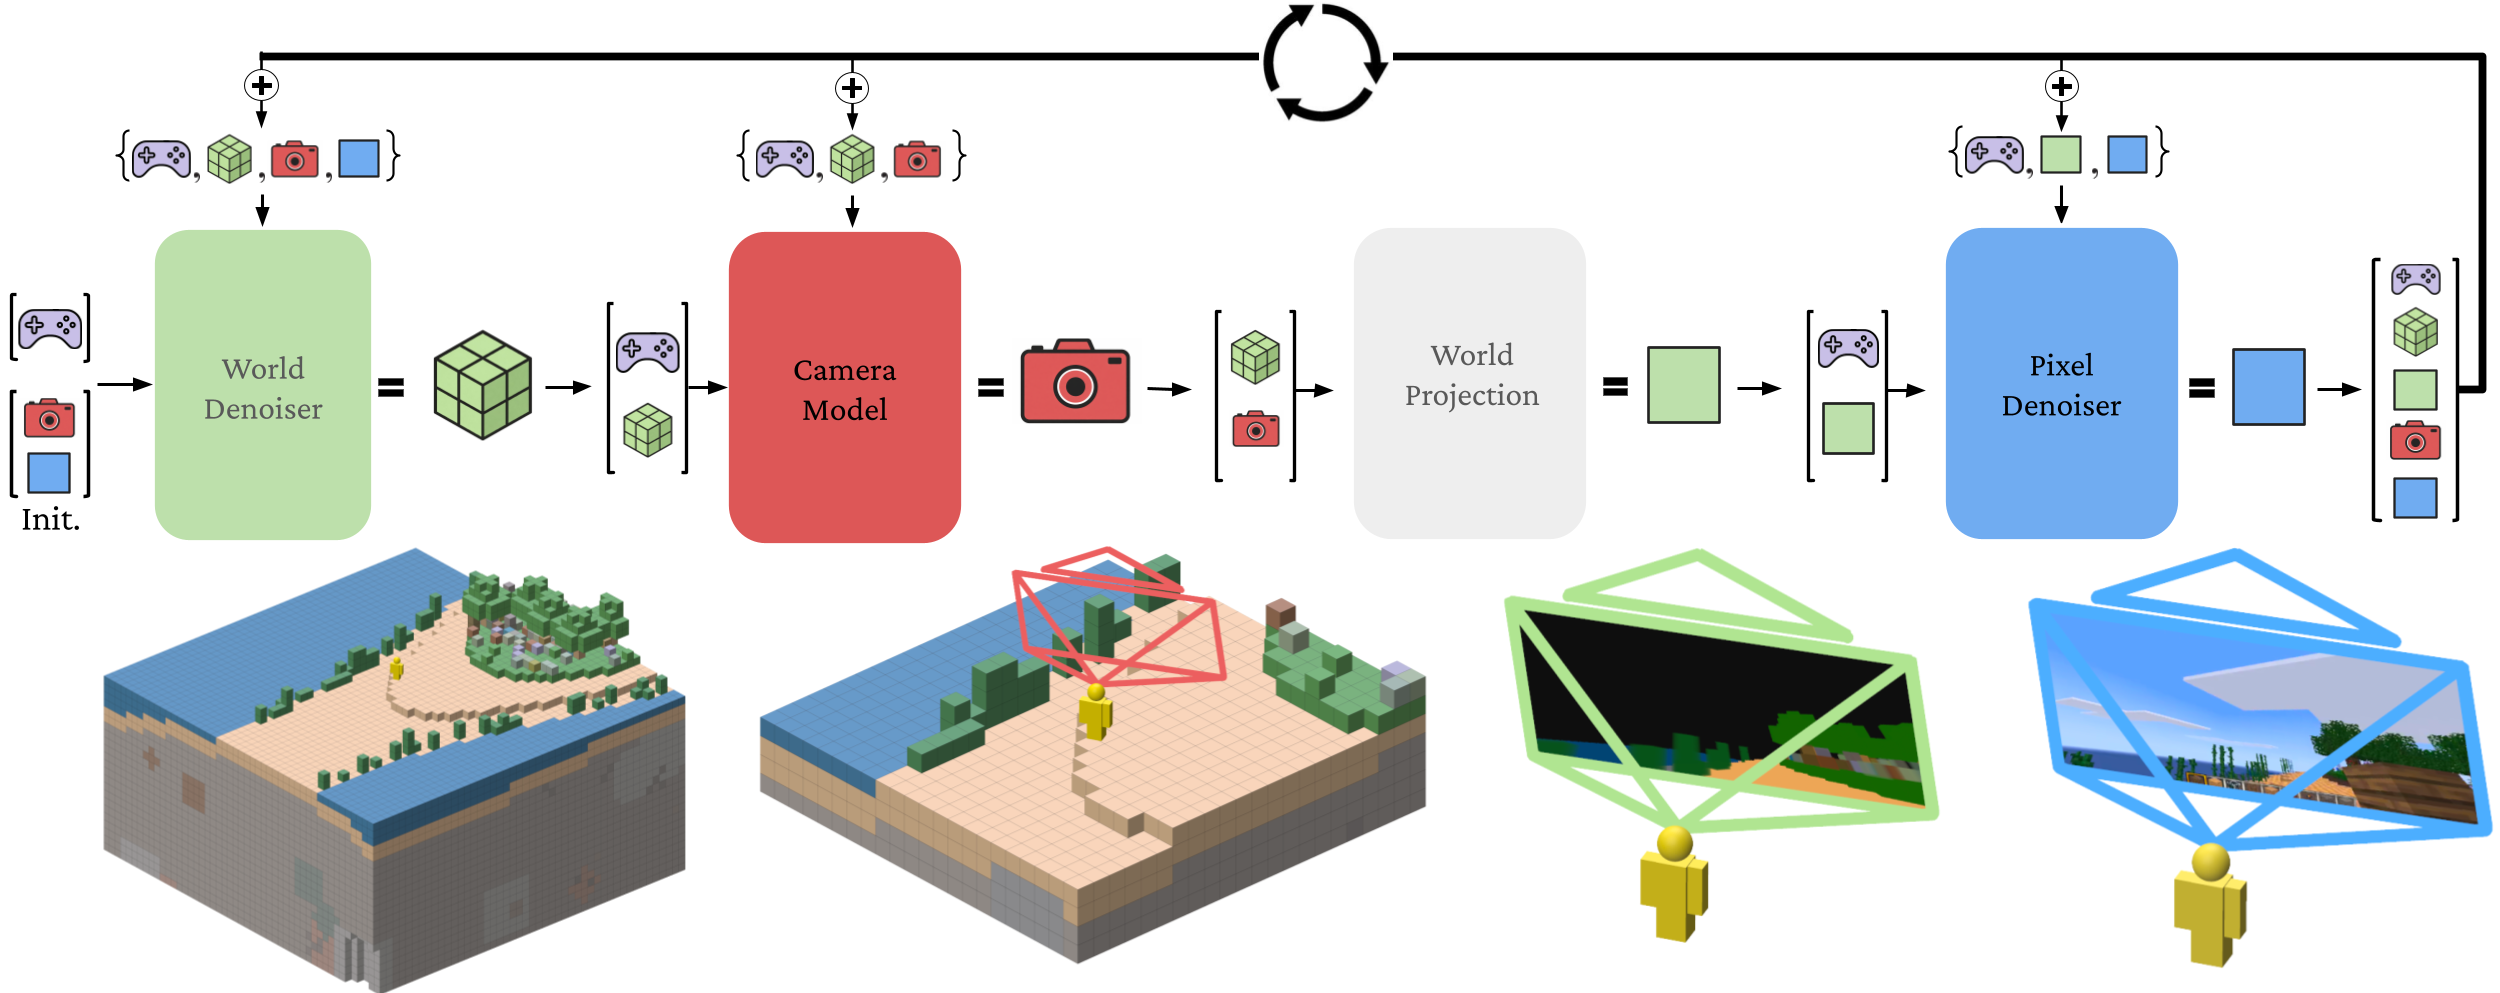
\includegraphics[width=\linewidth]{figs/Pipeline.png}}
    \caption{Initialized with a \DIFdelbeginFL \DIFdelFL{single-frame}\DIFdelendFL \DIFaddbeginFL \DIFaddFL{single pixel frame}\DIFaddendFL , PERSIST evolves in \DIFdelbeginFL \DIFdelFL{a four-part }\DIFdelendFL \DIFaddbeginFL \DIFaddFL{an }\DIFaddendFL auto-regressive loop in response to user actions 
\includegraphics[height=1.5ex]{figs/action.png}. We first denoise the 3D environment \DIFdelbeginFL \DIFdelFL{centered }\DIFdelendFL \DIFaddbeginFL \DIFaddFL{centred }\DIFaddendFL on the agent in the form of a latent \textit{world-frame} \DIFdelbeginFL %DIFDELCMD < 
\includegraphics[height=1.65ex]{figs/voxels.png}%%%
\DIFdelendFL \DIFaddbeginFL 
\includegraphics[height=1.85ex]{figs/voxels.png}\DIFaddendFL . Next, camera parameters 
\includegraphics[height=1.5ex]{figs/camera.png} are predicted with a feed-forward transformer. We then project the world to the camera plane to form a depth-ordered stack of world latents 
\includegraphics[height=1.5ex]{figs/voxel_frame.png}. Finally, pixel latents 
\includegraphics[height=1.5ex]{figs/pixel.png} are \DIFdelbeginFL \DIFdelFL{diffused}\DIFdelendFL \DIFaddbeginFL \DIFaddFL{denoised}\DIFaddendFL , \DIFdelbeginFL \DIFdelFL{conditioned on }\DIFdelendFL \DIFaddbeginFL \DIFaddFL{using }\DIFaddendFL pixel-aligned 3D information from the world \DIFdelbeginFL \DIFdelFL{frame}\DIFdelendFL \DIFaddbeginFL \DIFaddFL{latents stack }
\includegraphics[height=1.5ex]{figs/voxel_frame.png} \DIFaddFL{as guidance}\DIFaddendFL .}
    \DIFdelbeginFL %DIFDELCMD < \label{pipeline}
%DIFDELCMD <   %%%
\DIFdelendFL \DIFaddbeginFL \label{fig:pipeline}
  \DIFaddendFL \end{center}
\end{figure*}



\DIFdelbegin %DIFDELCMD < \begin{figure*}[ht]
%DIFDELCMD <   \vskip %%%
\DIFdelFL{0.2in
  }%DIFDELCMD < \begin{center}
%DIFDELCMD <     \centerline{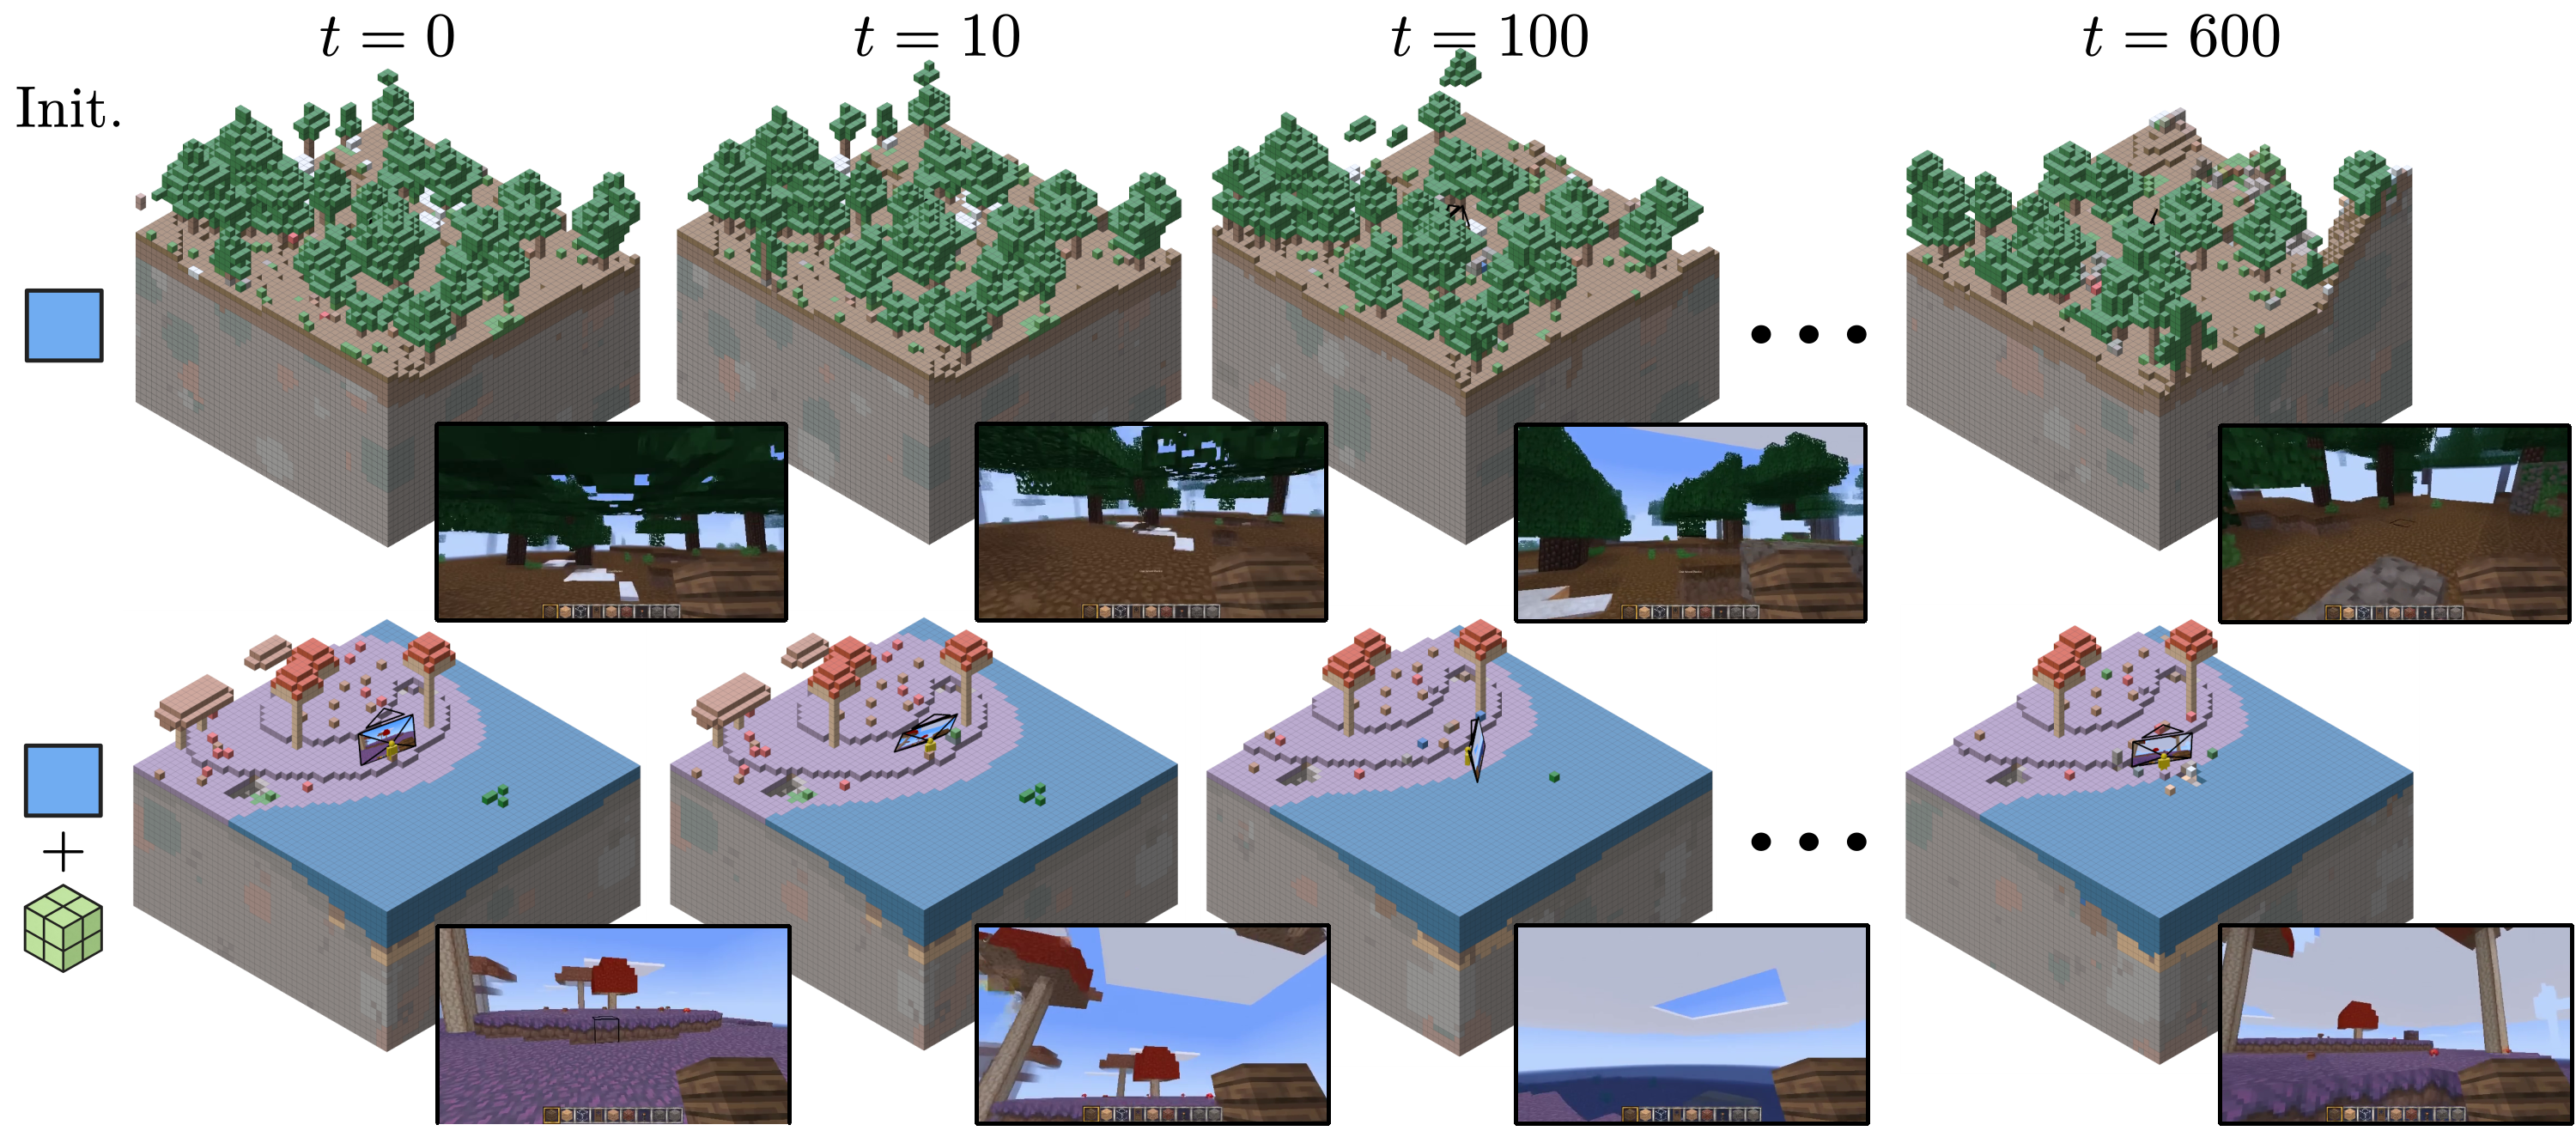
\includegraphics[width=\linewidth]{figs/qual.png}}
%DIFDELCMD <     %%%
%DIFDELCMD < \caption{%
{%DIFAUXCMD
\DIFdelFL{Initalize with a single RGB frame, we visualize the world-frames and videos produced by an auto-regressive rollout of 600 timesteps.}}
    %DIFAUXCMD
%DIFDELCMD < \label{rollout}
%DIFDELCMD <   \end{center}
%DIFDELCMD < \end{figure*}
%DIFDELCMD < 

%DIFDELCMD < %%%
\DIFdelend Interactive world models aim to generate experiences that unfold over time in response to user actions, enabling a new class of photo-realistic, personalised, and immersive interactive experiences for human users~\citep{kanervisto2025world, genie3, huang2025voyager}. At the same time, such models hold significant potential for safely training embodied agents within simulators learned directly from data~\citep{hafner2025training,micheli2023transformers,alonso2024diffusion,garcin2024dred}. Unlike passive video generation, interactive generation requires models to respond meaningfully to external interventions. In this setting, realism is not determined solely by per-frame visual quality, but by the degree to which the generated experience maintains persistent environments and stable dynamics throughout extended rollouts.

Most existing approaches to interactive video generation rely on auto-regressive (AR) models that condition on the history of past observations and actions to generate the most recent frame, often using \DIFdelbegin \DIFdel{diffusion- or flow-based }\DIFdelend \DIFaddbegin \DIFadd{diffusion-based }\DIFaddend transformers with causal attention~\cite{peebles2023scalable}.
This formulation is attractive: it naturally supports real-time action conditioning, allows generation to proceed indefinitely, and integrates cleanly with recent advances in large-scale video modelling.
As a result, AR video diffusion models form the backbone of many recent neural game engines and interactive world models~\DIFdelbegin \DIFdel{\mbox{%DIFAUXCMD
\citep{chegamegen,decart2024oasis,he2025matrix,xiao2025worldmem, valevskidiffusion,zhang2025matrix,yu2025gamefactory}}\hskip0pt%DIFAUXCMD
}\DIFdelend \DIFaddbegin \DIFadd{\mbox{%DIFAUXCMD
\citep{chegamegen,he2025matrix,valevskidiffusion,zhang2025matrix,yu2025gamefactory}}\hskip0pt%DIFAUXCMD
}\DIFaddend .

However, conditioning on high-dimensional visual observations is computationally expensive, and the number of prior frames that AR models can ingest is tightly constrained by hardware.
In practice, this limits AR generation to condition on what amounts to only a few seconds of past footage, even when observations are compressed to lower spatial and/or temporal resolutions using learned autoencoders.
As a result, a growing body of work has explored how best to populate this limited contextual window, most commonly through heuristic strategies that retrieve individual key frames from a memory bank of past observations~\citep{xiao2025worldmem,huang2025memory}.

Yet, an inherent flaw of key-frame retrieval methods is that each pixel observation provides only partial, highly redundant, and viewpoint-dependent information about the world at a fixed point in time.
As the memory bank grows, identifying the relevant past evidence becomes increasingly difficult.
As a result, generating extended \DIFaddbegin \DIFadd{and }\DIFaddend coherent experiences within complex 3D environments remains an open challenge even for frontier models.\footnote{\DIFdelbegin \DIFdel{While not independently verifiable, closed-source }\DIFdelend \DIFaddbegin \DIFadd{Closed-source frontier }\DIFaddend models \DIFdelbegin \DIFdel{have reported }\DIFdelend \DIFaddbegin \DIFadd{report }\DIFaddend achieving up to one minute of visual memory, representing the current \DIFdelbegin \DIFdel{claimed }\DIFdelend frontier of AR generation~\citep{genie3}.}

In this work, we propose to depart from pixel-based histories and substitute key frame retrieval with \textit{active key frame generation}.
We are inspired by traditional 3D simulators and game engines, which maintain coherence by directly rendering pixel frames from a persistent and dynamically evolving 3D state of the world. We \DIFdelbegin \DIFdel{present }\DIFdelend \DIFaddbegin \DIFadd{introduce }\DIFaddend PERSIST, a framework that brings persistence to learned AR world models \DIFdelbegin \DIFdel{.
}\DIFdelend \DIFaddbegin \DIFadd{by tracking a dynamic 3D representation of the environment. We describe our framework in \mbox{%DIFAUXCMD
\Cref{fig:pipeline}}\hskip0pt%DIFAUXCMD
.
}\DIFaddend PERSIST decomposes world simulation into three coupled components: a \textit{world-frame model} that predicts how \DIFdelbegin \DIFdel{an implicit, }\DIFdelend \DIFaddbegin \DIFadd{a }\DIFaddend learned representation of a \DIFdelbegin \DIFdel{physical scene in three dimensions }\DIFdelend \DIFaddbegin \DIFadd{3D scene }\DIFaddend evolves over time, a \textit{camera model} that \DIFdelbegin \DIFdel{predicts }\DIFdelend \DIFaddbegin \DIFadd{tracks }\DIFaddend the agent’s viewpoint within this scene, and a \textit{world-to-pixel generation module} that produces observations via differentiable projection and a learned rendering function.

Rather than treating pixels as the primary carrier of memory, PERSIST models \DIFdelbegin \DIFdel{both }\DIFdelend the structure and dynamics of the environment \DIFdelbegin \DIFdel{directly in }\DIFdelend \DIFaddbegin \DIFadd{in a }\DIFaddend latent 3D space.
This persistent world representation captures how the scene \DIFdelbegin \DIFdel{itself }\DIFdelend evolves over time, while the camera acts as a query mechanism that extracts the subset of 3D information relevant to guide the generation of the current frame.
This formulation enables long-horizon rollouts with fixed-cost memory, enforces geometric consistency by construction, and remains fully learned and compatible with modern \DIFdelbegin \DIFdel{diffusion- }\DIFdelend \DIFaddbegin \DIFadd{diffusion }\DIFaddend and flow-based training objectives.

We evaluate PERSIST in a \DIFdelbegin \DIFdel{large-scale voxel-based }\DIFdelend \DIFaddbegin \DIFadd{complex 3D }\DIFaddend environment and find that explicitly \DIFdelbegin \DIFdel{modeling }\DIFdelend \DIFaddbegin \DIFadd{modelling }\DIFaddend persistent 3D dynamics leads to substantially improved long-horizon generation quality compared to \DIFdelbegin \DIFdel{pixel-window }\DIFdelend \DIFaddbegin \DIFadd{rolling-window }\DIFaddend and memory-retrieval baselines.
Our approach exhibits stronger temporal stability, improved spatial memory when revisiting previously observed regions, and markedly better 3D consistency overall.
Beyond quantitative gains, persistent world representation enables new capabilities, including explicit 3D scene \DIFdelbegin \DIFdel{initialization%DIF < , mid-episode scene edits, 
}\DIFdelend \DIFaddbegin \DIFadd{initialisation, mid-episode scene edits, 
}\DIFaddend and the emergence of off-screen dynamic processes that continue to evolve even when not directly observed.

\section{Related Works}


%DIF < \paragraph{Rectified flow models.}
\DIFaddbegin \begin{figure*}[ht]
  \begin{center}
    \centerline{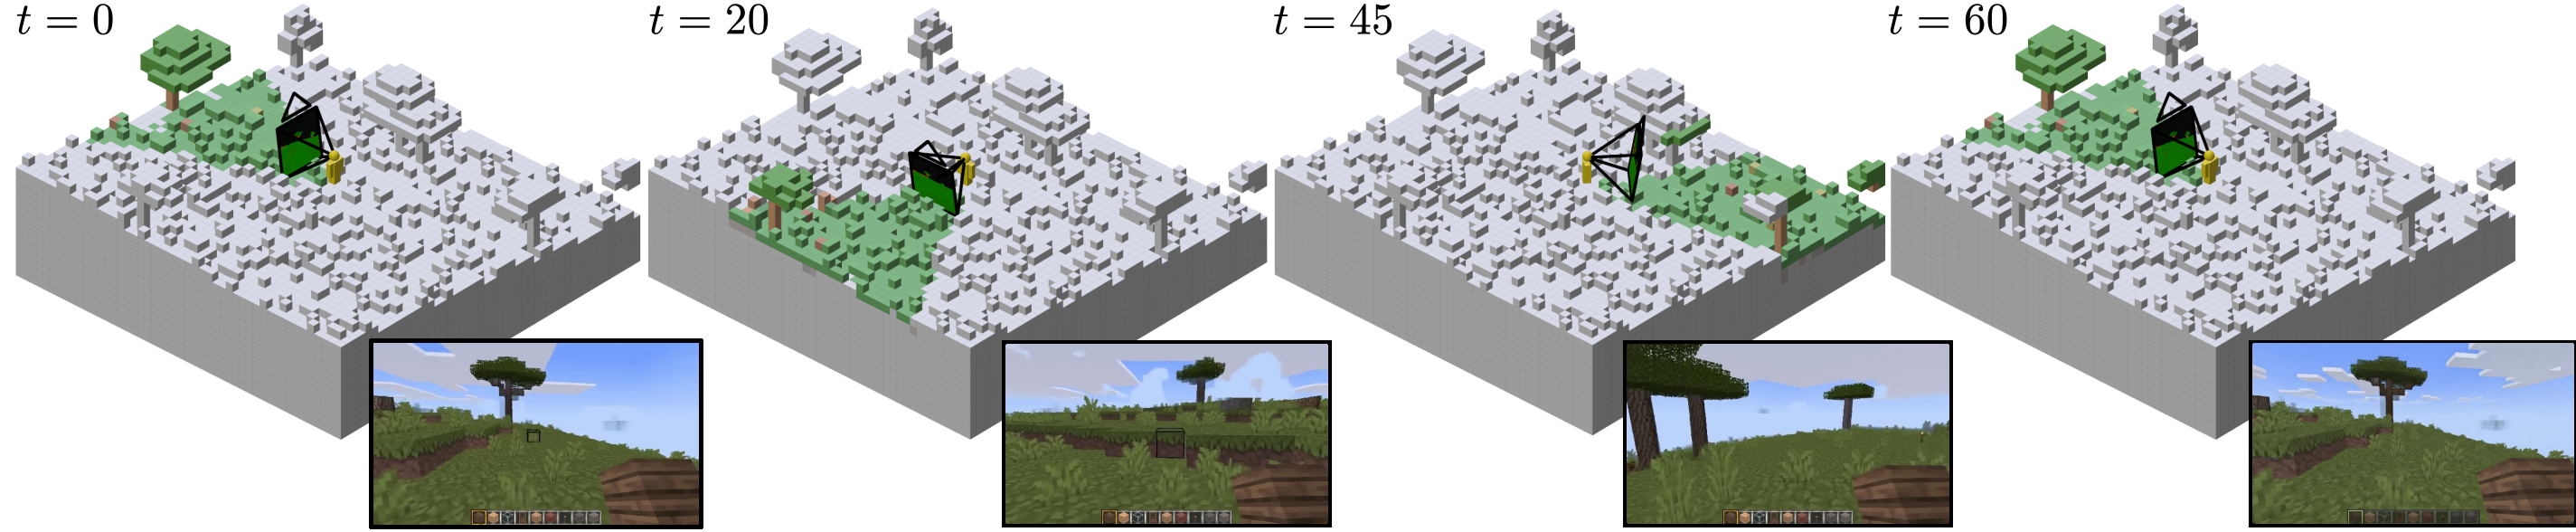
\includegraphics[width=\linewidth]{figs/rotate_rgb.png}}
    \caption{\DIFaddFL{PERSIST enables long-horizon spatial memory by modelling the dynamics of a 3D world-frame }
\includegraphics[height=2ex]{figs/voxels.png} \DIFaddFL{around the agent. Camera parameters }
\includegraphics[height=1.5ex]{figs/camera.png} \DIFaddFL{then act as memory look-up key, fetching relevant features from the world frame via a geometric projection (here visualized as the coloured voxels).}} 
    \label{fig:rollout-rotate}
    \vspace{-0.5cm}
  \end{center}
\end{figure*}

%DIF > \textbf{Rectified flow models.}
\DIFaddend %Rectified flow treats generation as learning a velocity field that transports noise to data with low-variance supervision and efficient sampling~\citep{lipman2022flow}. This objective has been shown to be compatible with transformer backbones and latent-space training, and integrates with DiT-style architectures~\citep{peebles2023scalable}. Leveraging this compatibility, we parameterise both world-frame and pixel-space denoisers as conditional rectified flow models, thereby enabling action-conditioned denoising given a fixed context. This formulation supports efficient per-step updates that preserve training stability while reducing inference cost, while also keeping a single objective across modules and horizons.

\DIFdelbegin \paragraph{\DIFdel{Video denoising models.}}
%DIFAUXCMD
\addtocounter{paragraph}{-1}%DIFAUXCMD
\DIFdel{Recent advances in denoising models have led to substantial progress in video generation, extending image synthesis techniques to produce temporally coherent videos.
Recent methods adopt transformer-based designs, but are limited to denoising short clips due to the poor scaling of attention with video length. To address this, auto-regressive video generation has emerged as a promising direction for extending video sequences.
In this setting, rather than diffusing an entire sequence at a fixed noise level, frames are denoised sequentially, enabling potentially unbounded generation.
}\DIFdelend %DIF >  \textbf{Video denoising models.}
%DIF >  Recent advances in denoising models have led to substantial progress in video generation, extending image synthesis techniques to produce temporally coherent videos.
%DIF >  Recent methods adopt transformer-based designs~\citep{peebles2023scalable}, but are limited to generating short video clips, due to the poor scaling of attention with video length. Auto-regressive video generation denoises frames sequentially, and has emerged as a promising direction for extending video sequences indefinitely~\citep{huang2025self}.

\DIFdelbegin \paragraph{\DIFdel{World models.}} %DIFAUXCMD
\addtocounter{paragraph}{-1}%DIFAUXCMD
\DIFdel{In parallel, world models}\DIFdelend %DIF > mention key-frame retrieval in this sentence?
\DIFaddbegin \textbf{\DIFadd{World models.}} \DIFadd{World models~\mbox{%DIFAUXCMD
\citep{https://doi.org/10.5281/zenodo.1207631} }\hskip0pt%DIFAUXCMD
}\DIFaddend aim to simulate environments by predicting future states conditioned on user actions\DIFdelbegin \DIFdel{, providing a foundation for model-based learning. Advances }\DIFdelend \DIFaddbegin \DIFadd{. Recent progress }\DIFaddend in video generation \DIFdelbegin \DIFdel{have enabled }\DIFdelend \DIFaddbegin \DIFadd{models enable }\DIFaddend high-fidelity interactive \DIFdelbegin \DIFdel{world simulation}\DIFdelend \DIFaddbegin \DIFadd{simulation~\mbox{%DIFAUXCMD
\citep{genie3,alonso2024diffusion,decart2024oasis}}\hskip0pt%DIFAUXCMD
}\DIFaddend . However, \DIFdelbegin \DIFdel{due to limited context windows, existing methods have to discard previously generated content, leading to temporal inconsistency and challenges with long-term spatial memory. Recently, interactive world models have employed spatially-informed voting mechanisms to retrieve relevant frames. }\DIFdelend \DIFaddbegin \DIFadd{maintaining spatial and temporal consistency over extended rollouts remains challenging due to the finite number of past frames existing models can incorporate as context. Prior works propose to alleviate this limitation via spatio-temporal compression of input tokens ~\mbox{%DIFAUXCMD
\citep{hafner2025training}}\hskip0pt%DIFAUXCMD
, memory-efficient attention mechanisms~\mbox{%DIFAUXCMD
\citep{po2025long} }\hskip0pt%DIFAUXCMD
or by populating the model context window with frames sampled from the full generation history~\mbox{%DIFAUXCMD
\citep{song2025history}}\hskip0pt%DIFAUXCMD
. Among this latter class of approaches, \mbox{%DIFAUXCMD
\cite{xiao2025worldmem,huang2025memory} }\hskip0pt%DIFAUXCMD
propose sampling strategies that retrieve key-frames according to their spatial relevance. Nevertheless, such methods rely on retrieving relevant information from an ever-growing history of pixel observations, a task that becomes increasingly difficult and costly over extended rollouts. In contrast, PERSIST retrieves contextual information directly from a dynamically evolving 3D latent state, making its information retrieval mechanism independent of episode length.
}\DIFaddend 

\DIFdelbegin \paragraph{\DIFdel{3D Scene models}}
%DIFAUXCMD
\addtocounter{paragraph}{-1}%DIFAUXCMD
%DIFDELCMD < 

%DIFDELCMD < %%%
%DIF <  \todo[inline]{ <- May want a better title than that. Talk about models that generate a renderable 3D scene [e.g. Trellis, or its extension]. Sometimes it's explorable [e.g. Voyager, Worldlabs' paper etc]. But the scene is not interactive / dynamic. Instead we predict the dynamic 3D state of the world, modelling both dyamics processes (e.g. water flowing [if you want to give an example]) and player interacting with environment (e.g. player swimming, climbing [stop short of mentioning destroying / creating parts of the environment as we don't have conclusive proof for that capability yet.]) }
%DIFDELCMD < 

%DIFDELCMD < %%%
\DIFdel{Unlike static }\DIFdelend \DIFaddbegin \textbf{\DIFadd{3D environment representations.}} \DIFadd{In parallel, a growing number of approaches incorporate explicit }\DIFaddend 3D \DIFdelbegin \DIFdel{scene representations such as TRELLIS~\mbox{%DIFAUXCMD
\citep{xiang2024structured}}\hskip0pt%DIFAUXCMD
, which focuses on generating high-fidelity geometry, our work focuses on the prediction of a dynamic }\DIFdelend \DIFaddbegin \DIFadd{representations into their generative architectures to produce explorable and spatially consistent environments~\mbox{%DIFAUXCMD
\citep{huang2025voyager,marble,zhou2025learning}}\hskip0pt%DIFAUXCMD
. However, these environments remain static, restricting interaction to basic navigation within a frozen world. In contrast, PERSIST learns a }\DIFaddend 3D \DIFdelbegin \DIFdel{world state}\DIFdelend \DIFaddbegin \DIFadd{representation that evolves over time, enabling it to capture dynamic processes occurring within the environment, and richer agent–environment interactions}\DIFaddend .
\DIFdelbegin \DIFdel{While recent advances in explorable environments such as World Labs~\mbox{%DIFAUXCMD
\citep{worldlab} }\hskip0pt%DIFAUXCMD
or Voyager~\mbox{%DIFAUXCMD
\citep{huang2025voyager} }\hskip0pt%DIFAUXCMD
allow for consistent navigation through a staticscene, they often lack the capability to model complex and time-varying processes. Our approach goes beyond passive observation by modeling both intrinsic environmental dynamics and agent-environment interactions.
By predicting the evolution of the underlying 3D state rather than just the visual surface, we enable a level of temporal and spatial consistency that reflects the active, changing nature of a truly interactive world.
}\DIFdelend 

\DIFdelbegin \paragraph{\DIFdel{Neural rendering.}} %DIFAUXCMD
\addtocounter{paragraph}{-1}%DIFAUXCMD
\DIFdel{In recent years, }\DIFdelend \DIFaddbegin \textbf{\DIFadd{Neural rendering.}} \DIFadd{While }\DIFaddend neural radiance fields \DIFdelbegin \DIFdel{have seen increasing usage in computer graphics as a compact }\DIFdelend \DIFaddbegin \DIFadd{(NeRFs) have become a popular, compact, }\DIFaddend and resolution-free \DIFdelbegin \DIFdel{parameterization }\DIFdelend \DIFaddbegin \DIFadd{representation }\DIFaddend of 3D scenes~\citep{mildenhall2021nerf, muller2022instant, li2023neuralangelo}\DIFdelbegin \DIFdel{.
Popularized by NeRF~\mbox{%DIFAUXCMD
\citep{mildenhall2021nerf}}\hskip0pt%DIFAUXCMD
, these techniques rely on expensive ray-marching of an implicit function. We take inspiration from a real-time graphics technique known as }\textit{\DIFdel{deferred shading}}%DIFAUXCMD
\DIFdel{~\mbox{%DIFAUXCMD
\citep{deering1988triangle}}\hskip0pt%DIFAUXCMD
: a mesh is first rasterized into a }\DIFdelend \DIFaddbegin \DIFadd{, they rely on costly ray marching with many neural network queries, making them prohibitively expensive for interactive use. PERSIST instead takes inspiration from neural deferred shading, which rasterizes explicit geometry into }\DIFaddend screen-space \DIFdelbegin \DIFdel{map of geometric information, which is then decoded pixel-wise into RGB values using a screen-space shader. 
Recently, learned neural deferred shaders~\mbox{%DIFAUXCMD
\citep{thies2019deferred, worchel2022multi, walker2023explicit} }\hskip0pt%DIFAUXCMD
have proved to be efficient alternatives to ray-marching based neural renderers.
By leveraging highly-optimized polygon rasterization pipelines, they can achieve interactive frame rates across a wide range of compute platforms, including mobile devices~\mbox{%DIFAUXCMD
\citep{chen2023mobilenerf}}\hskip0pt%DIFAUXCMD
.
However, these approaches have not seen much adoption due to their restriction to a fixed topology during training.
In this work, we assume a fixed topology in the form of grid mesh, on which geometric features can be efficiently rasterized. %DIF < \todo[inline]{WIP}
}\DIFdelend \DIFaddbegin \DIFadd{features and decodes them with learned neural shaders, enabling more efficient rendering~\mbox{%DIFAUXCMD
\citep{thies2019deferred, worchel2022multi, walker2023explicit, chen2023mobilenerf, deering1988triangle}}\hskip0pt%DIFAUXCMD
.
%DIF >  \textbf{Neural rendering.} In recent years, neural radiance fields have seen increasing usage in computer graphics as a compact and resolution-free parametrisation of 3D scenes~\citep{mildenhall2021nerf, muller2022instant, li2023neuralangelo}.
%DIF >  Popularized by NeRF~\citep{mildenhall2021nerf}, these techniques rely on expensive ray-marching of an implicit function.
%DIF >  We instead take inspiration from a real-time graphics technique known as \textit{deferred shading}~\citep{deering1988triangle}: a mesh is first rasterized into a screen-space map of geometric information, which is then decoded pixel-wise into RGB values using a screen-space shader. 
%DIF >  Recently, learned neural deferred shaders~\citep{thies2019deferred, worchel2022multi, walker2023explicit, chen2023mobilenerf} have proved to be efficient alternatives to ray-marching based neural renderers.
%DIF > By leveraging highly-optimized polygon rasterization pipelines, they can achieve interactive frame rates across a wide range of compute platforms, including mobile devices~\citep{chen2023mobilenerf}.
%DIF > While these approaches have not seen much adoption due to their restriction to a fixed topology, we instead assume a fixed grid mesh of latent features, which are rasterized and processed by learned denoiser. %\todo[inline]{WIP}
}\DIFaddend 

\section{Preliminaries}

\DIFaddbegin \begin{figure*}[ht]
  \begin{center}
    \centerline{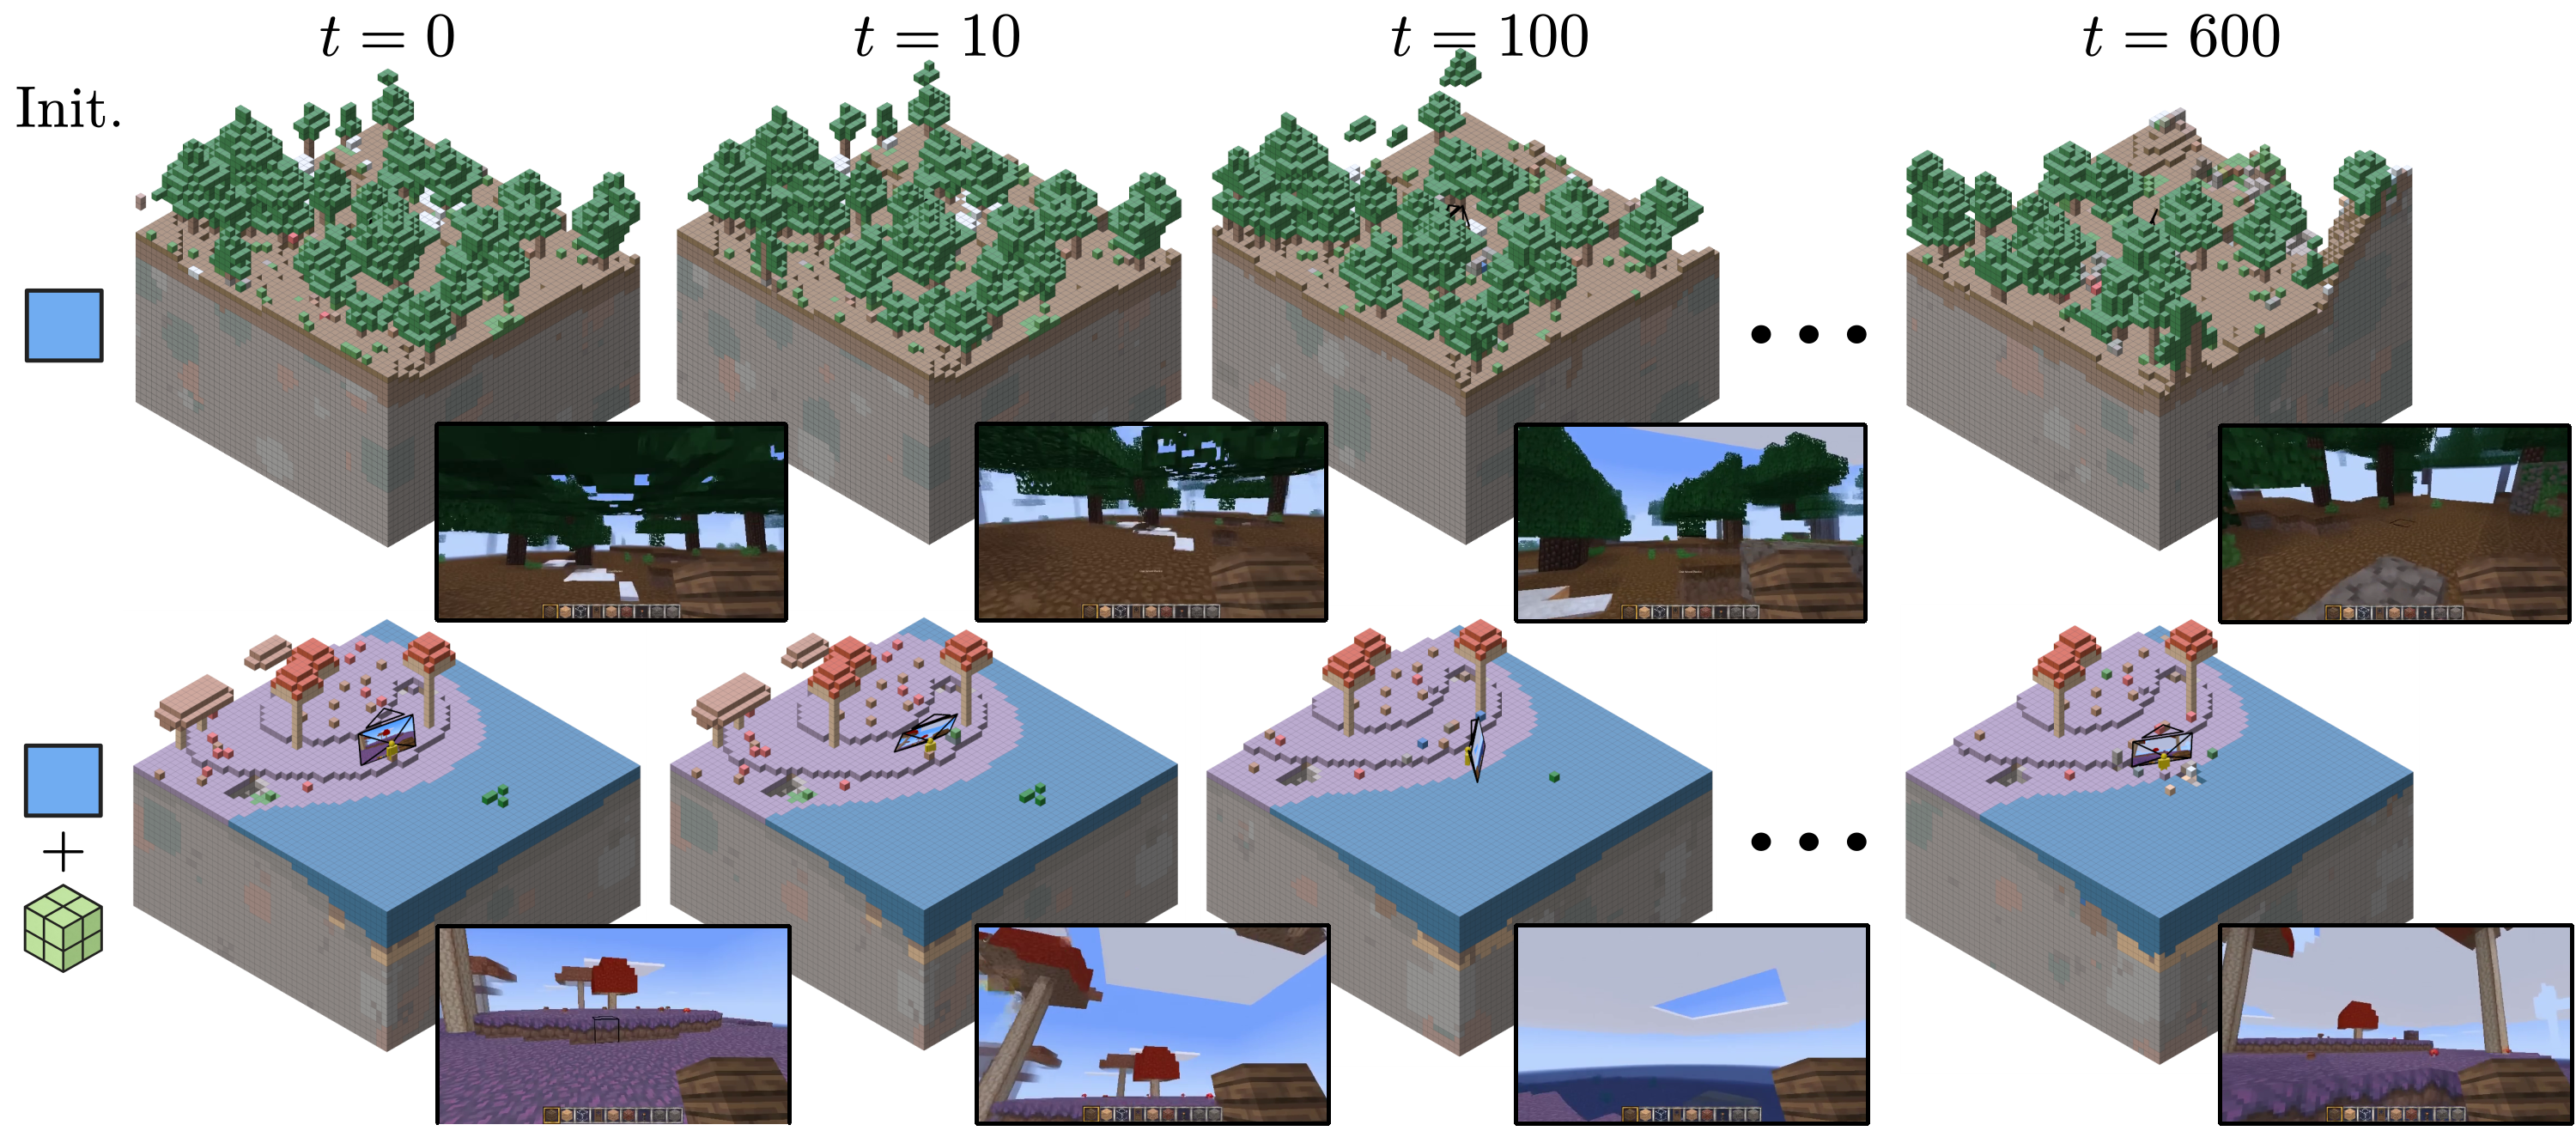
\includegraphics[width=\linewidth]{figs/qual.png}}
    \caption{\DIFaddFL{PERSIST can be initialized with a single RGB frame (}
\includegraphics[height=1.5ex]{figs/pixel.png}\DIFaddFL{, row 1), or with a single RGB and world frame (}
\includegraphics[height=1.5ex]{figs/pixel.png} \DIFaddFL{+ }
\includegraphics[height=2ex]{figs/voxels.png}\DIFaddFL{, row 2). We visualize the world-frames and videos produced by an auto-regressive rollout of 600 timesteps. Even with a single RGB frame for initialization, PERSIST can generate cohesive and evolving worlds.}}
    \label{fig:rollout-voxel}
     \vspace{-0.2cm}
  \end{center}
\end{figure*}

\DIFaddend \textbf{Rectified flow matching.} Our approach is based on the paradigm of flow matching and diffusion models~\citep{lipman2022flow}, where the task is to restore a clean data sample $x^0$ given a noised version $x^\tau$.
The noise level $\tau \in [0, 1]$ determines the degree of corruption of the data, where $\tau=0$ denotes clean data and $\tau=1$ indicates pure noise.
Rectified flow models~\citep{lipman2022flow,albergo2023building} employ a noising process $x^\tau = (1-\tau)x^0 + \tau x^1$ that linearly interpolates between sample $x^0$ and noise $x^1 \sim \mathcal{N}(0,\sI)$. 
Provided with a noised sample and corresponding noise level, the model $\gV_\theta$ is trained to predict the velocity vector $v = x^0 - x^1$ pointing towards the clean data via the conditional flow matching objective (CFM)~\citep{lipman2022flow}: 
\begin{equation}
    \mathcal{L}(\theta) = \norm{\gV_\theta (x^\tau, \tau) - (x^0 - x^1)}^2 \quad \tau \sim p(\tau),
\end{equation}
where $\tau$ is often sampled from a uniform or logit-normal distribution.
During inference, random noise $x^1$ is iteratively denoised into a clean sample $x^0$ over $K$ sampling steps, with uniform or variable step size $d^k$:
%
\begin{equation}
    x^{\tau - d^k} = x^\tau + \gV_\theta (x^\tau, \tau) d^k, \quad \tau \leftarrow \tau - d^k.
\end{equation}
\textbf{Autoregressive video generation.} While full-sequence video diffusion models treat videos as a single data sample to be denoised jointly at inference time, AR models treat videos as a sequence of individual frames $X^{n}_1 = x_1,x_2,\dots,x_n$ to be diffused sequentially.\footnote{Notation-wise, the noise level of an individual frame $x^\tau_t$ is indicated by superscript $\tau$, its position in the sequence by subscript $t$.
In the case of a truncated sequence $X_k^{t}$, we overload the notation to have $k$ and $t$ indicate its beginning and end.} AR models employ causal masking strategies during training to ensure no information travels from the future into the past. Diffusion forcing~\citep{chen2024diffusion}
improves the generation stability of AR video diffusion models at inference by introducing per-frame noise levels that are sampled independently during training.
At inference, AR generation becomes a special case of the training setup, where the current frame is iteratively denoised from random noise and past frames receive a small fixed noise level $\tau_\text{ctx}$.

\textbf{Interactive world simulation.} Because generation proceeds step-by-step, AR models can in principle be unrolled indefinitely and conditioned on external control signals provided at each timestep.
This enables a transition from passive video generation to interactive world simulation. \DIFdelbegin %DIFDELCMD < 

%DIFDELCMD < %%%
\DIFdelend We employ a similar formalism as~\citet{valevski2024diffusionmodelsrealtimegame} to characterize the problem of learning a \textit{world model}, which we define here as a learned simulator of some \textit{interactive environment} $\mathcal{E}$\DIFdelbegin \DIFdel{.
$\mathcal{E}$ is specified by the tuple $\langle \mathbb{S}, \mathbb{O}, \mathbb{A}, \Omega, p\rangle$, }\DIFdelend \DIFaddbegin \DIFadd{:
}\begin{equation}
    \DIFadd{\mathcal{E} = \langle \mathbb{S} , \mathbb{O}, \mathbb{A}, \Omega, p\rangle,
}\end{equation}
 \DIFaddend where $\mathbb{S}$ is the space of latent states, $\mathbb{O}$ the space of observations, $\mathbb{A}$ the set of actions that may be taken within the environment, $\Omega : \mathbb{S} \rightarrow \mathbb{O}$ a partial projection function mapping states to \DIFdelbegin \DIFdel{actions and }\DIFdelend \DIFaddbegin \DIFadd{observations, }\DIFaddend $p(s^\prime|a,s)$ is a transition probability function such that $s,s^\prime \in \mathbb{S}\times\mathbb{S}$ and $a \in \mathbb{A}$. 
Given a distribution of initial states \DIFaddbegin \DIFadd{$p_0$ }\DIFaddend and episode length \DIFdelbegin \DIFdel{$p_0$ and }\DIFdelend $N_0$, a policy $\pi$ in charge of selecting actions in $\mathcal{E}$\DIFaddbegin \DIFadd{, }\DIFaddend and a distance metric between observation sequences $D : \mathbb{O}^n \times \mathbb{O}^n \rightarrow \mathbb{R}$, learning an interactive world simulation of $\mathcal{E}$ consists of minimising the objective $\mathbb{E}[D(O^n, \tilde{O}^n)]$\DIFdelbegin \DIFdel{, where }\DIFdelend \DIFaddbegin \DIFadd{. }\DIFaddend $O^n$ is a sequence of observations of length $n\sim N_0$ collected in $\mathcal{E}$ from starting state $s_0\sim p_0$ and by following $\pi$; and $\tilde{O}^n$ is obtained from an AR model $\gQ_\theta$ initialised at $\vo_0 = \Omega(s_0)$ and subjected to the same action sequence.

\section{A Persistent Environment Representation}
Learning \DIFaddbegin \DIFadd{an auto-regressive model }\DIFaddend $\gQ_\theta$ is often challenging when $\mathcal{E}$ is a complex 3D environment featuring high dimensional pixel observations.
First, memory constraints limit $\gQ_\theta$ to condition on a \DIFdelbegin \DIFdel{limited }\DIFdelend \DIFaddbegin \DIFadd{finite }\DIFaddend context window of past $K$ frames, \DIFdelbegin \DIFdel{imposing a constraint on }\DIFdelend \DIFaddbegin \DIFadd{which degrades }\DIFaddend temporal consistency once the generated episode exceeds \DIFdelbegin \DIFdel{$K$}\DIFdelend \DIFaddbegin \DIFadd{this horizon}\DIFaddend . 
Second, pixel observations \DIFdelbegin \DIFdel{generally }\DIFdelend \DIFaddbegin \DIFadd{typically }\DIFaddend provide partial information about the environment's hidden state, \DIFdelbegin \DIFdel{which can make learning }\DIFdelend \DIFaddbegin \DIFadd{making learning accurate }\DIFaddend transition dynamics challenging.
%DIF < (for example when taking backwards steps while facing forwards). 
\DIFdelbegin \DIFdel{One solution would be }\DIFdelend \DIFaddbegin \DIFadd{One might therefore attempt }\DIFaddend to have $\gQ_\theta$ \DIFdelbegin \DIFdel{track }\DIFdelend \DIFaddbegin \DIFadd{condition on some approximation of }\DIFaddend the hidden state $s$\DIFdelbegin \DIFdel{. However, }\DIFdelend \DIFaddbegin \DIFadd{; however }\DIFaddend $s$ \DIFdelbegin \DIFdel{may }\DIFdelend \DIFaddbegin \DIFadd{can }\DIFaddend be arbitrarily complex \DIFdelbegin \DIFdel{and/or not measurable --- }\DIFdelend \DIFaddbegin \DIFadd{or entirely unmeasurable. Even if $s$ was accessible, learning the observation function $\Omega : \sS \rightarrow \sO $ to recover observations can be a comparably challenging problem. For example, }\DIFaddend in the case of a video game, $s$ \DIFdelbegin \DIFdel{represents the internal state of the game engine and its dynamic memory content.
Even if $s$ could be tracked, approximating $\Omega$ to recover the observation may be just as difficult}\DIFdelend \DIFaddbegin \DIFadd{would be the program's dynamic memory contents, which may not be particularly helpful for easily recovering pixel observations}\DIFaddend . 

Instead, we define a proxy $\tilde{s} = \langle \vw, \vc \rangle$, where $\vw$ is a \textit{world-frame} representing a fixed region of space \DIFdelbegin \DIFdel{centered }\DIFdelend \DIFaddbegin \DIFadd{centred }\DIFaddend on the agent, and $\vc$ \DIFdelbegin \DIFdel{encodes }\DIFdelend \DIFaddbegin \DIFadd{is a camera state encoding }\DIFaddend the agent's view within $\vw$.
Although not a perfect replacement for the \DIFaddbegin \DIFadd{true }\DIFaddend hidden state, \DIFdelbegin \DIFdel{we argue that tracking }\DIFdelend $\tilde{s}$ is \DIFdelbegin \DIFdel{a highly effective modeling }\DIFdelend \DIFaddbegin \DIFadd{an effective modelling }\DIFaddend choice when $\mathcal{E}$ is a 3D environment, as it lets us:
\DIFdelbegin %DIFDELCMD < 

%DIFDELCMD < %%%
\DIFdelend %DIF > todo reduce spacing [noitemsep]
\DIFaddbegin \begin{enumerate}
    \item \DIFaddend \textbf{Simplify information retrieval.} \DIFdelbegin \DIFdel{At timestep $t$, }\DIFdelend \DIFaddbegin \DIFadd{\mbox{%DIFAUXCMD
\Cref{fig:rollout-rotate} }\hskip0pt%DIFAUXCMD
demonstrates how the world-frame }\DIFaddend $\vw_t$ \DIFdelbegin \DIFdel{takes on the role of }\DIFdelend \DIFaddbegin \DIFadd{can function as a dynamic }\DIFaddend \textit{spatial memory} \DIFdelbegin \DIFdel{, while }\DIFdelend \DIFaddbegin \DIFadd{module throughout the episode, while the camera state }\DIFaddend $\vc_t$ acts as a \DIFdelbegin \DIFdel{lookup-key to extract spatial information from }\DIFdelend \DIFaddbegin \textit{\DIFadd{spatial lookup-key }} \DIFadd{to retrieve the spatial information in }\DIFaddend $\vw_t$ \DIFdelbegin \DIFdel{directly relevant to }\DIFdelend \DIFaddbegin \DIFadd{that is necessary to reconstruct }\DIFaddend $\vo_t$. \DIFdelbegin %DIFDELCMD < 

%DIFDELCMD < %%%
\DIFdelend \DIFaddbegin \DIFadd{$\vc_t$ encodes the information to project this information to screen-space, without requiring explicit knowledge of the true observation function.
    }\item \DIFaddend \textbf{Improve dynamics predictions.} Tracking $\vw$ and $\vc$ \DIFdelbegin \DIFdel{simplifies }\DIFdelend \DIFaddbegin \DIFadd{over time facilitates }\DIFaddend modelling dynamics that \DIFdelbegin \DIFdel{would prove challenging under partial observability}\DIFdelend \DIFaddbegin \DIFadd{are difficult to infer from pixel observations alone}\DIFaddend , such as interactions \DIFaddbegin \DIFadd{or collisions }\DIFaddend with out-of-view objects\DIFdelbegin \DIFdel{(e.g. modelling collisions)}\DIFdelend , or tracking how occluded regions of the environment change over time.
\DIFaddbegin \end{enumerate}
\DIFaddend 




\section{\DIFdelbegin \DIFdel{Methodology}\DIFdelend \DIFaddbegin \DIFadd{PERSIST}\DIFaddend }
%DIF <  \todo[inline]{Algo to describe sampling process of $\gQ_\theta$, complements figure 1 and describes different initialisation modes}
We present PERSIST (Persistent Environment Representations for Simulating Interactive Space-Time), a world simulation framework for complex 3D environments.
PERSIST decomposes the world simulation objective into the tasks of \textit{world frame prediction}, \textit{camera prediction} and \textit{world-to-pixel generation}.

\textbf{\DIFdelbegin \DIFdel{Data }\DIFdelend \DIFaddbegin \DIFadd{Dataset construction and }\DIFaddend pre-processing.} The different components of PERSIST are trained from a dataset of trajectories collected from $\mathcal{E}$.
A trajectory consists of a sequence of pixel observations $O$, actions $A$, world-frames $W$ and camera views $C$.
In this work, we assume that $W$ and $C$ are directly obtainable from $\mathcal{E}$, the former as a 3D voxel grid \DIFdelbegin \DIFdel{encoding semantic information }\DIFdelend within a cuboid centered on the agent, and the later as a vector encoding the camera intrinsics and extrinsics.
Actions are embedded as a 23-dimensional multi-hot encoding of key presses and discretised mouse movements.
We train \DIFdelbegin \DIFdel{two separate VAEs (P-VAE and W-VAE) to encode base }\DIFdelend \DIFaddbegin \DIFadd{a 2D-VAE and a 3D-VAE to encode }\DIFaddend pixel- and world-frames into latent patches $\bar{\vo}$ and $\bar{\vw}$ of 10$\times$10 pixels and $4^3$ voxels respectively. 

\subsection{World-Frame and Camera Prediction}

\textbf{World frame prediction.} At each timestep, a new world-frame is generated by sampling 
\begin{equation}
  \bar{\vw}_t \sim \gW_\theta(\DIFdelbegin %DIFDELCMD < \bar{\vw_t} %%%
\DIFdelend \DIFaddbegin \bar{\rvw_t} \DIFaddend | \bar{W}^{t-1}_{t-K}, A^t_{t-K}, C^{t-1}_{t-K-1}, \bar{O}^{t-1}_{t-K-1}),  
\end{equation}
where $K$ is the model's temporal context window and latents $\bar{W}^{t-1}_{t-K}$ and $\bar{O}^{t-1}_{t-K-1}$ are encoded using the VAEs. 
$\gW_\theta$ is \DIFdelbegin \DIFdel{parameterised }\DIFdelend \DIFaddbegin \DIFadd{parametrised }\DIFaddend as a rectified flow model with a causal Diffusion Transformer (DiT) backbone~\citep{peebles2023scalable} employing interleaved spatial, temporal and cross-attention modules\DIFaddbegin \DIFadd{~\mbox{%DIFAUXCMD
\citep{decart2024oasis}}\hskip0pt%DIFAUXCMD
}\DIFaddend .
We modify \DIFdelbegin \DIFdel{spatial modules }\DIFdelend \DIFaddbegin \DIFadd{the spatial module }\DIFaddend to handle three spatial dimensions, and replace RoPE spatial embeddings~\citep{su2024roformer} with absolute position embeddings of the XYZ coordinates of the centroid of each voxel token.
We keep the temporal module as-is.
Actions and cameras are jointly embedded using a multi-layer perceptron (MLP).
The resulting embeddings are added to the denoising timestep embedding and injected into each module via Adaptive Layer Normalisation (AdaLN)~\citep{peebles2023scalable}.
We \DIFaddbegin \DIFadd{employ Pl\"ucker embeddings~\mbox{%DIFAUXCMD
\citep{xiao2025worldmem,sitzmann2021light} }\hskip0pt%DIFAUXCMD
to }\DIFaddend convey information on how individual pixel patches project to 3D space\DIFdelbegin \DIFdel{via Pl\"ucker embeddings ~\mbox{%DIFAUXCMD
\citep{xiao2025worldmem,sitzmann2021light} }\hskip0pt%DIFAUXCMD
which we compute from the cameras and concatenate to the channel dimension of the }\DIFdelend \DIFaddbegin \DIFadd{. These embeddings are computed from $C^{t-1}_{t-K-1}$ and are concatenated channel-wise to the }\DIFaddend pixel patches.
The resulting patches are then injected \DIFdelbegin \DIFdel{via }\DIFdelend \DIFaddbegin \DIFadd{into the model via the }\DIFaddend cross-attention \DIFaddbegin \DIFadd{module}\DIFaddend .
Finally, we \DIFaddbegin \DIFadd{employ the 3D-VAE to }\DIFaddend decode $\bar{\vw}_t$ \DIFdelbegin \DIFdel{back }\DIFdelend to its native resolution\DIFdelbegin \DIFdel{using the W-VAE}\DIFdelend .

Crucially, $\gW_\theta$ supports conditioning on $\bar{W}=\varnothing$, making it able of generating \DIFdelbegin \DIFdel{the }\DIFdelend \DIFaddbegin \DIFadd{an }\DIFaddend initial world frame $\vw_0$ from initial condition \DIFdelbegin \DIFdel{$\langle \bar{\vo}_0, \vc_0 \rangle$ }\DIFdelend \DIFaddbegin \DIFadd{$\langle \vo_0, \vc_0 \rangle$ }\DIFaddend at inference time.
Thus, while we rely on $W$ to train $\gW_\theta$, we do not have to rely on ground truth 3D conditioning during inference. \DIFaddbegin \DIFadd{We provide examples for each inference configuration in \mbox{%DIFAUXCMD
\Cref{fig:rollout-voxel}}\hskip0pt%DIFAUXCMD
.
}\DIFaddend 


% \textbf{Dynamic loss.}

\textbf{Camera model.} At any given timestep, cameras are represented as the 10-dimensional vector \DIFdelbegin \DIFdel{$\vc = [\textbf{pos}, \textbf{rot}, \text{fov}]$}\DIFdelend \DIFaddbegin \DIFadd{$\vc = \langle\textbf{pos}, \textbf{rot}, \text{fov}\rangle$}\DIFaddend , where $\textbf{pos}\in \sR^3$ encodes the camera's position in the world-frame\DIFaddbegin \DIFadd{, }\DIFaddend $\textbf{rot}\in \sR^6$ its orientation as a 6D continuous rotation~\citep{zhou2019continuity}, and $\text{fov}\in \sR$ its field-of-view. The camera model predicts $\vc_{t} = \gC_\theta (C^{t-1}_{t-1-K}, W^t_{t-K}, A^t_{t-K})$ using a 1D causal transformer backbone with RoPE temporal embeddings. Individual tokens are obtained by passing $\textbf{pos}$ and $\textbf{rot}$  through separate positional embedders, concatenating $\text{fov}$ and applying a linear projection. $W$ is cropped to its inner-most $4^3$ voxels and embedded alongside $A$ via a joint MLP prior to AdaLN injection. Given that the camera only rotates along its pitch and yaw axis, we re-parametrise the model's output layer to predict \DIFdelbegin \DIFdel{$\bar{\vc}=[\textbf{pos}, \Delta\textbf{rot}, \Delta\text{fov}]$}\DIFdelend \DIFaddbegin \DIFadd{$\bar{\vc}=\langle \textbf{pos}, \Delta\text{pitch}, \Delta\text{yaw}, \Delta\text{fov}\rangle$}\DIFaddend , with residuals \DIFdelbegin \DIFdel{$\Delta\textbf{rot} = (\text{pitch}_t - \text{pitch}_{t-1},\text{yaw}_t - \text{yaw}_{t-1}) \in \sR^2$ }\DIFdelend \DIFaddbegin \DIFadd{$\Delta\text{pitch} = \text{pitch}_t - \text{pitch}_{t-1}$,$\Delta\text{yaw} =\text{yaw}_t - \text{yaw}_{t-1}$ }\DIFaddend and $\Delta \text{fov}=\text{fov}_t - \text{fov}_{t-1}$.\footnote{$\vc_t$ is recovered from $\langle \bar{\vc}_t, \vc_{t-1}\rangle$ via an algebraic manipulation at inference time.} The camera model is trained via MSE losses applied to \DIFdelbegin \DIFdel{$\textbf{pos}$, $\textbf{rot}$ and $\text{fov}$ with different coefficients}\DIFdelend \DIFaddbegin \DIFadd{each component of $\bar{\vc}$}\DIFaddend .

\subsection{World-to-Pixel Generation}
\DIFaddbegin 

\DIFaddend In order to condition the pixel-space generation on 3D information we need to form world-to-pixel correspondence.

\textbf{World \DIFdelbegin \DIFdel{Projection}\DIFdelend \DIFaddbegin \DIFadd{projection}\DIFaddend .} %DIF < need to define what a rasteriser is either here or earlier in the text
\DIFdelbegin \DIFdel{Since we model a camera $\vc$ and 3D world-frame }\DIFdelend \DIFaddbegin \DIFadd{We project }\DIFaddend $\vw$ \DIFdelbegin \DIFdel{, we can provide $\mathcal{P}_\theta$ with pixel-level conditioning on the relevant 3D features $\vw$ via a differentiable projection $\mathcal{R}(\vc, \vw)$ }\DIFdelend to screen-space \DIFdelbegin \DIFdel{. We then leave the final rendering step as a learned process for the screen-space denoiser $\mathcal{P}_\theta$. This choice allows the pixel denoiser to learn arbitrary compositing functions, whilst still enforcing geometric consistency through analytic projections of the 3D world.
}%DIFDELCMD < 

%DIFDELCMD < \vspace{-0.35cm}
%DIFDELCMD < \begin{figure}[h]
%DIFDELCMD <     \centering
%DIFDELCMD < 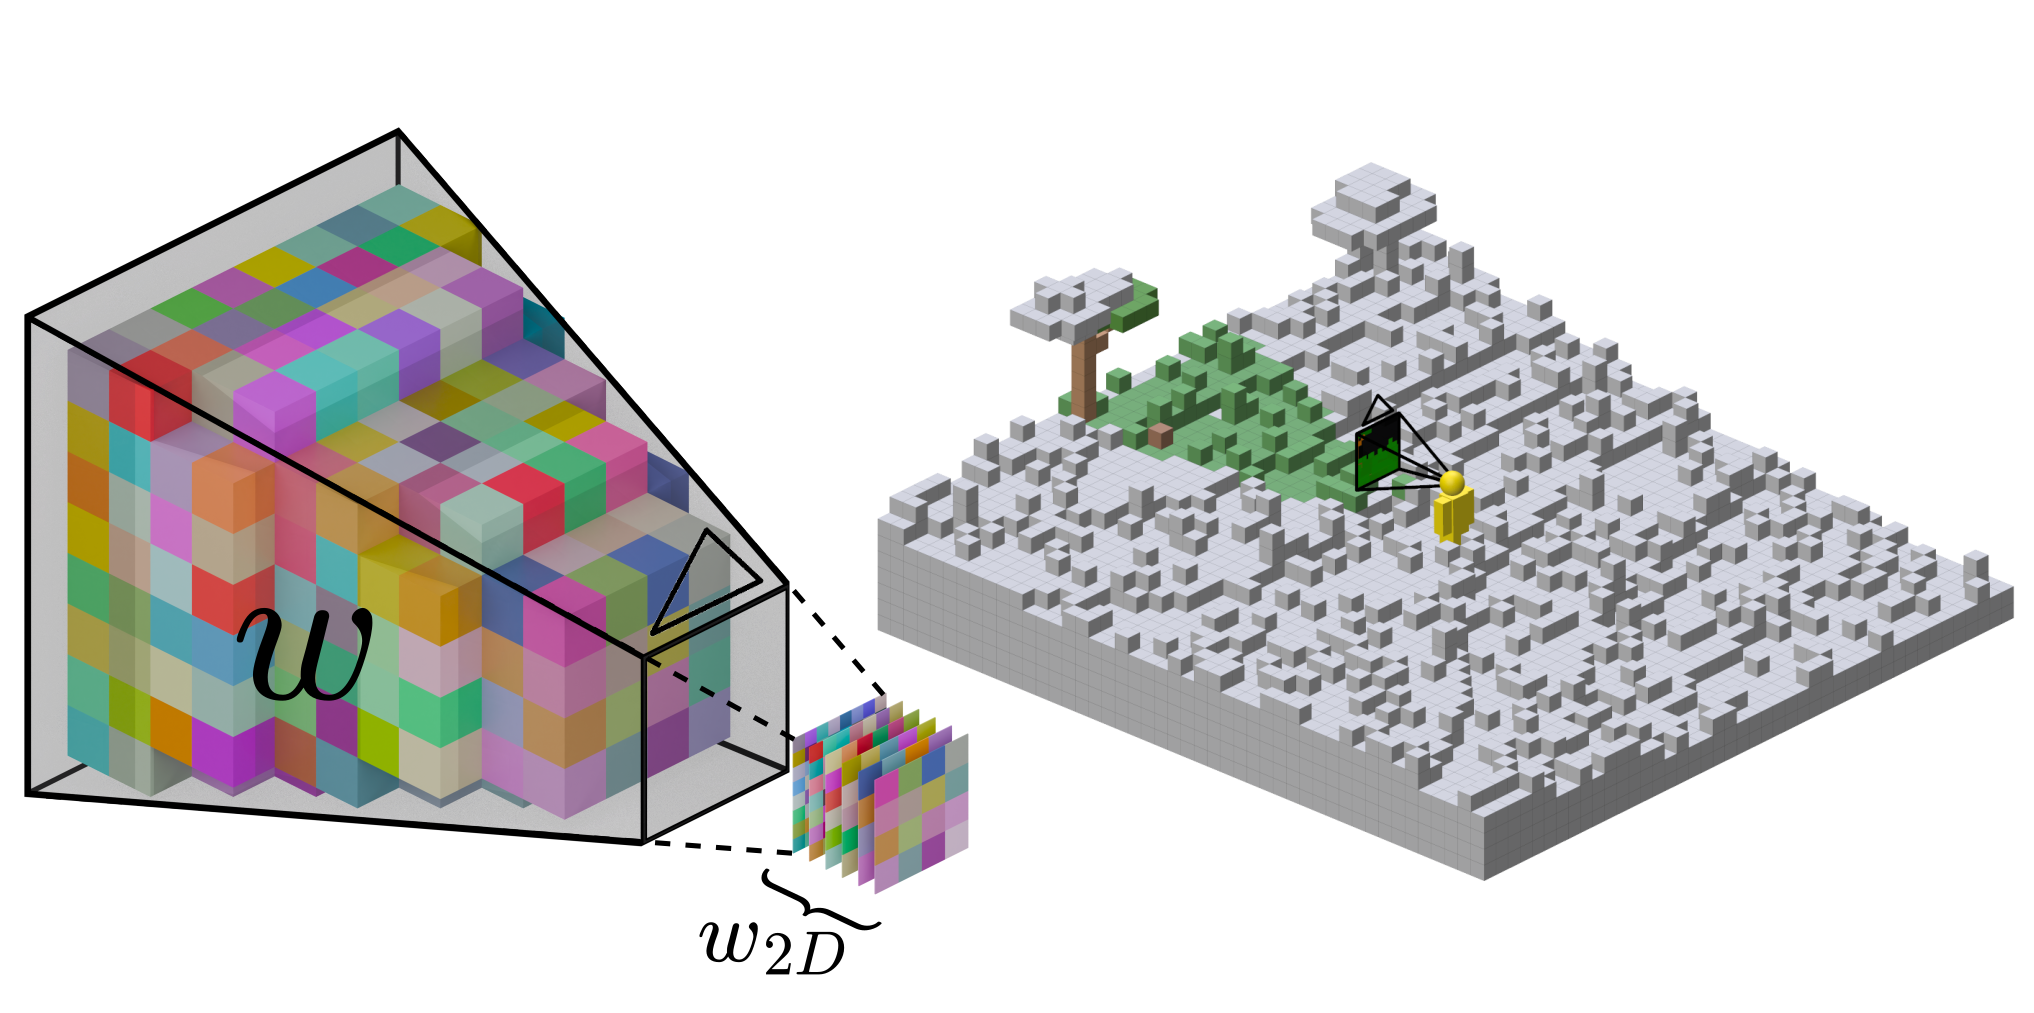
\includegraphics[width=1\linewidth]{figs/renderer_w.png}
%DIFDELCMD <     %%%
%DIFDELCMD < \caption{%
{%DIFAUXCMD
\DIFdelFL{(Left) world frame $\vw$ features are projected to screen-space to form a depth-ordered stack of features $\vw_{2D}$. (Right) the world region fetched by the camera projection is displayed in colour.}}
    %DIFAUXCMD
%DIFDELCMD < \label{fig:placeholder}
%DIFDELCMD < \end{figure}
%DIFDELCMD < 

%DIFDELCMD < %%%
\DIFdel{We define the projection operator $\mathcal{R}$ as 
}\DIFdelend \DIFaddbegin \DIFadd{via the projection operator }\DIFaddend \begin{equation}
    \mathcal{R}(\vc, \vw) = (\DIFdelbegin %DIFDELCMD < \vw%%%
\DIFdelend \DIFaddbegin \tilde{\vw}\DIFaddend _{2D}, \vd), 
\end{equation}
where \DIFdelbegin \DIFdel{$\vw_{2D}  \in \mathbb{R}^{h \times w \times l \times m}$  represents }\DIFdelend \DIFaddbegin \DIFadd{$\tilde{\vw}_{2D}  \in \mathbb{R}^{h \times w \times l \times m}$ is }\DIFaddend a per-pixel \DIFdelbegin \DIFdel{depth-sorted }\DIFdelend \DIFaddbegin \DIFadd{depth-ordered }\DIFaddend list of $l$ voxel features with $m$ channels, \DIFdelbegin \DIFdel{and }\DIFdelend \DIFaddbegin \DIFadd{indexed according to their position in screen space $\langle h_i, w_j\rangle$. }\DIFaddend $\vd \in \mathbb{R}^{h \times w \times l}$ \DIFdelbegin \DIFdel{are their respective linear depths }\DIFdelend \DIFaddbegin \DIFadd{is the linear depth of each voxel feature }\DIFaddend measured in camera space. \DIFdelbegin \DIFdel{To ensure pixel-level alignment between 2D and 3D latents, we rasterize $\vw$ using }\DIFdelend \DIFaddbegin \DIFadd{We provide a visualisation of how $\mathcal{R}$ constructs $\tilde{\vw}_{2D}$ and $\vd$ in \mbox{%DIFAUXCMD
\Cref{fig:render}}\hskip0pt%DIFAUXCMD
. $\mathcal{R}$ employs }\DIFaddend the same $h,w$ \DIFaddbegin \DIFadd{screen }\DIFaddend dimensions as the pixel latents\DIFdelbegin \DIFdel{. For projection, we use the CUDA-accelerated differentiable rasterization 
provided by~\mbox{%DIFAUXCMD
\citep{Laine2020diffrast}}\hskip0pt%DIFAUXCMD
. For details, please see the appendix. }\DIFdelend \DIFaddbegin \DIFadd{, ensuring pixel-level alignment with $\bar{\vo}$. Finally, we combine $\tilde{\vw}_{2D}$ and $\vd$ into $\vw_{2D}\in \mathbb{R}^{h \times w \times z}$ via channel-wise concatenation, where $z = l \times (m+1)$. %DIF > We use the CUDA-accelerated differentiable rasterization provided by~\citep{Laine2020diffrast} to generate $(\vw_{2D}, \vd)$ via a fixed-cost, single feedforward operation.
}\DIFaddend 


%DIF <  For projecting, we leverage GPU-native triangle rasterization, by assigning voxel features to faces of a static voxel-grid mesh. Then, depth-peeling can applied during rasterization to produce a per-pixel, depth-ordered stack of 3D features $V_{2D}^{t} \in \mathbb{R}^{H \times W \times L \times C}$, where $L$ is the maximum number of layers. Since the mesh topology is fixed for a given resolution, we construct it once at initialization, updating vertex attributes ``on-the-fly" to avoid redundant mesh construction.  
%DIF >  Since we model a camera $\vc$ and 3D world-frame $\vw$, we can provide $\mathcal{P}_\theta$ with pixel-level conditioning on the relevant 3D features $\vw$ via a differentiable projection $\mathcal{R}(\vc, \vw)$ to screen-space. We then leave the final rendering step as a learned process for the screen-spa3ce denoiser $\mathcal{P}_\theta$. This choice allows the pixel denoiser to learn arbitrary compositing functions, whilst still enforcing geometric consistency through analytic projections of the 3D world.
%DIF >  We define the projection operator $\mathcal{R}$ as 
%DIF >  \begin{equation}
%DIF >      \mathcal{R}(\vc, \vw) = (\vw_{2D}, \vd), 
%DIF >  \end{equation}
%DIF >  where $\vw_{2D}  \in \mathbb{R}^{h \times w \times l \times m}$ represents a per-pixel depth-ordered list of $l$ voxel features with $m$ channels, indexed according to their position in screen space $\langle h_i, w_j\rangle$. $\vd \in \mathbb{R}^{h \times w \times l}$ represents the linear depth of each voxel feature measured in camera space. To ensure pixel-level alignment between 2D and 3D latents, we rasterize $\vw$ using the same $h,w$ screen dimensions as the pixel latents. For projection, we use the CUDA-accelerated differentiable rasterization 
%DIF >  provided by~\citep{Laine2020diffrast}. For details, please see the appendix.

\DIFdelbegin \DIFdel{While surrounding works~\mbox{%DIFAUXCMD
\cite{xiao2025worldmem,huang2025memory} }\hskip0pt%DIFAUXCMD
use $\vc_t$ to retrieve a relevant key frame from a memory bank of past pixel observations, PERSIST employs $\mathcal{R}$ to }\textit{\DIFdel{generate}} %DIFAUXCMD
\DIFdel{a key-frame from $\vw_t$ via a fixed-cost single feedforward operation.
}\DIFdelend \DIFaddbegin \begin{figure}[ht]
    \centering
    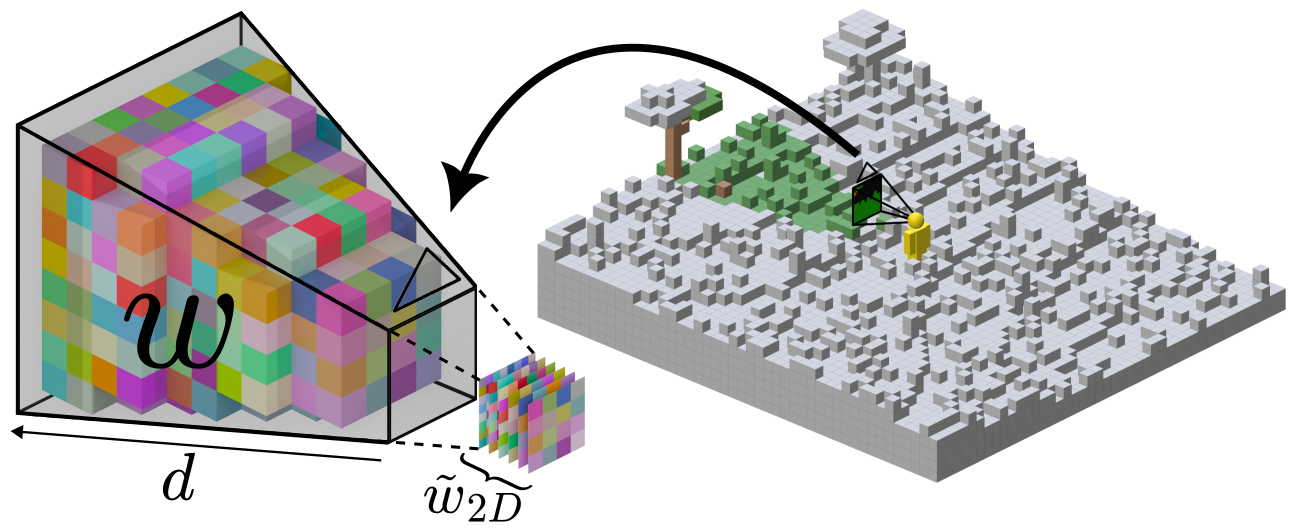
\includegraphics[width=0.9\linewidth]{figs/renderer.png}
    \vspace{-0.1cm}
    \caption{\DIFaddFL{World frame $\vw$ features are projected to screen-space to obtain the depth-ordered stack of features $\tilde{\vw}_{2D}$ and linear depth information $\vd$.}}
        \vspace{-0.2cm}
    \label{fig:render}
\end{figure}
\DIFaddend 



 

%DIF >  While surrounding works~\cite{xiao2025worldmem,huang2025memory} employ camera tracking to retrieve a key frame from a memory bank of past pixel observations, $\mathcal{R}$ lets PERSIST \textit{generate} a new key frame from the current world-frame representation $\vw_t$ via a fixed-cost, single feedforward operation.
\DIFaddbegin 

\DIFaddend \textbf{\DIFdelbegin \DIFdel{Screen space denoising}\DIFdelend \DIFaddbegin \DIFadd{Pixel frame prediction}\DIFaddend .}
\DIFdelbegin \DIFdel{Finally, the pixel frame is obtained by sampling
}\DIFdelend \DIFaddbegin \DIFadd{Pixel frames are generated by sampling
}\DIFaddend \begin{equation}
    \bar{\vo}_t \sim \gP_\theta (\DIFdelbegin %DIFDELCMD < \bar{\vo}%%%
\DIFdelend \DIFaddbegin \bar{\rvo}\DIFaddend _t | {W_{2D}}_{t-K}^{t}, A^t_{t-K}, \bar{O}^{t-1}\DIFdelbegin \DIFdel{_{t-K-1}}\DIFdelend \DIFaddbegin \DIFadd{_{t-K}}\DIFaddend )\DIFdelbegin \DIFdel{.
}\DIFdelend \DIFaddbegin \DIFadd{,
}\DIFaddend \end{equation}
\DIFdelbegin \DIFdel{$\gP_\theta$ is parameterized as a rectified flow model with a casual DiT backbone employing interleaved spatial and temporal modules. Actions are embedded using a MLP and injected via AdaLN. }\DIFdelend \DIFaddbegin \DIFadd{where ${W_{2D}}_{t-K}^{t}$ is obtained from the projection $\gR(C_{t-K}^{t},W_{t-K}^{t})$. }\DIFaddend Here, $\gP_\theta$ acts as a learned deferred shader\DIFdelbegin \DIFdel{, predicting }\DIFdelend \DIFaddbegin \DIFadd{~\mbox{%DIFAUXCMD
\cite{thies2019deferred} }\hskip0pt%DIFAUXCMD
which additionally predicts }\DIFaddend information not provided by 3D latents (e.g. texture, lighting\DIFdelbegin \DIFdel{and }\DIFdelend \DIFaddbegin \DIFadd{, }\DIFaddend particle effects, screen-space overlays\DIFdelbegin \DIFdel{)}\DIFdelend \DIFaddbegin \DIFadd{, \ldots). This choice allows $\gP_\theta$ to learn arbitrary rendering functions, whilst encouraging spatial consistency through its dependency on $\vw_{2D}$}\DIFaddend . \DIFdelbegin %DIFDELCMD < 

%DIFDELCMD < %%%
\DIFdel{Being directly projected in screen space, }\DIFdelend \DIFaddbegin \DIFadd{$\gP_\theta$ is parametrised as a rectified flow model with a causal DiT backbone employing interleaved spatial and temporal modules~\mbox{%DIFAUXCMD
\citep{decart2024oasis}}\hskip0pt%DIFAUXCMD
. Actions are embedded using a MLP and injected via AdaLN. }\DIFaddend $\vw_{2D}$ \DIFdelbegin \DIFdel{provides pixel-aligned information and can be  directly incorporated to $\bar{\vo}$ via a channel-wise concatenation. We first append channel-wise the depth information $\vd$ }\DIFdelend \DIFaddbegin \DIFadd{is projected }\DIFaddend to \DIFdelbegin \DIFdel{$\vw_{2D}$, and project the resulting vector to }\DIFdelend latent space via a \DIFaddbegin \DIFadd{channel-wise }\DIFaddend 1D-convolution \DIFaddbegin \DIFadd{and is incorporated to $\bar{\vo}$ via channel-wise concatenation}\DIFaddend . Crucially, we assign more latent channels to $\vw_{2D}$ than to $\bar{\vo}$, in order to bias the model to use the 3D latent frame as its primary source of information.

\subsection{Mitigating Exposure Bias}

During training, the denoisers condition on latents encoded from the training data. However, \DIFaddbegin \DIFadd{they condition on autoregressive predictions }\DIFaddend at inference time, \DIFdelbegin \DIFdel{the 3D denoiser }\DIFdelend \DIFaddbegin \DIFadd{leading to exposure bias~\mbox{%DIFAUXCMD
\citep{ning2023elucidating}}\hskip0pt%DIFAUXCMD
. We train each diffuser with diffusion forcing~\mbox{%DIFAUXCMD
\citep{chen2024diffusion} }\hskip0pt%DIFAUXCMD
to make them robust to the exposure bias induced by their own predictions. In addition, at inference $\gW_\theta$ }\DIFaddend depends on latents predicted by \DIFdelbegin \DIFdel{the pixel denoiser}\DIFdelend \DIFaddbegin \DIFadd{$\gP_\theta$}\DIFaddend , and vice-versa. To alleviate the resulting distributional shift\DIFdelbegin \DIFdel{caused by the denoisers' imperfect predictions}\DIFdelend , we apply a flat 10\% random noise augmentation to $\bar{O}$ when training $\gW_\theta$, and to $\bar{W}$ when training $\gP_\theta$. This lets us train each \DIFdelbegin \DIFdel{denoiser }\DIFdelend \DIFaddbegin \DIFadd{component of PERSIST }\DIFaddend separately and combine them at inference time \DIFdelbegin \DIFdel{, }\DIFdelend without any fine-tuning\DIFdelbegin \DIFdel{being necessary}\DIFdelend .

\section{Experiments}

\DIFdelbegin %DIFDELCMD < \begin{figure*}[ht]
%DIFDELCMD <   \vskip %%%
\DIFdelFL{0.2in
  }%DIFDELCMD < \begin{center}
%DIFDELCMD <     \centerline{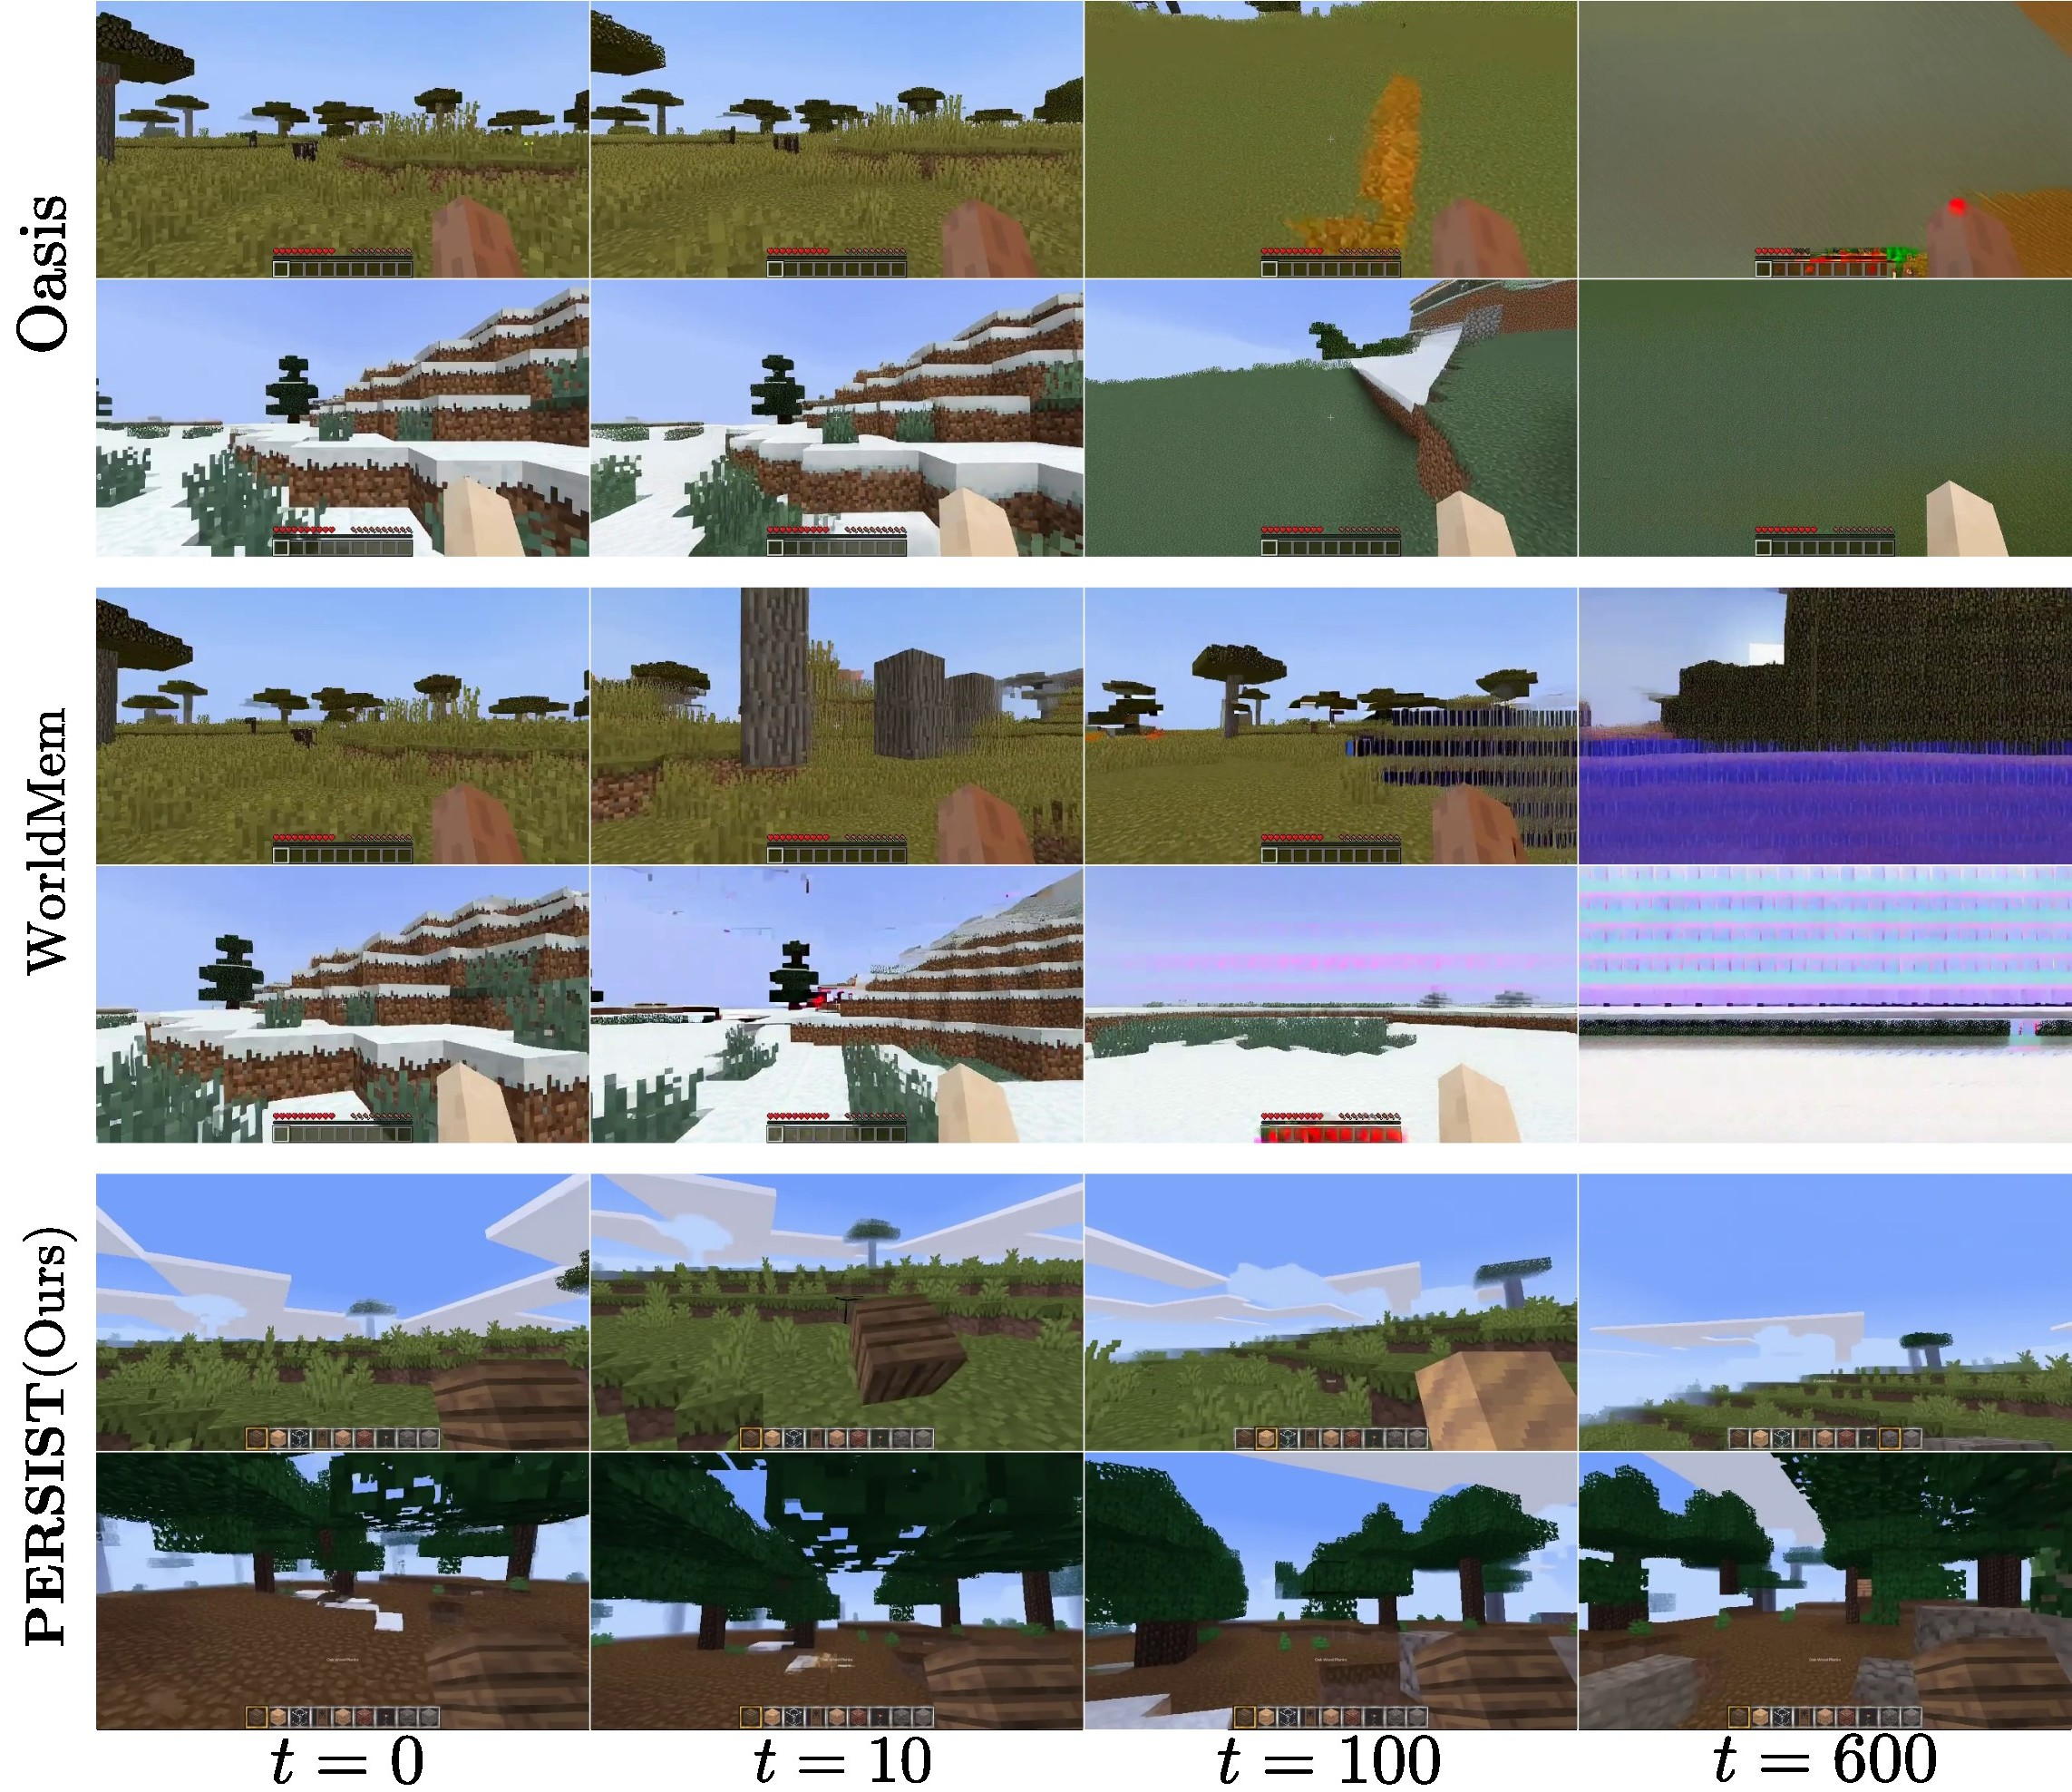
\includegraphics[width=\linewidth]{figs/compare.jpg}}
%DIFDELCMD <     %%%
%DIFDELCMD < \caption{%
{%DIFAUXCMD
\DIFdelFL{Qualitative Comparison between PERSIST (Ours), Oasis~\mbox{%DIFAUXCMD
\citep{decart2024oasis} }\hskip0pt%DIFAUXCMD
and WorldMem~\mbox{%DIFAUXCMD
\citep{xiao2025worldmem}}\hskip0pt%DIFAUXCMD
.}}
    %DIFAUXCMD
%DIFDELCMD < \label{rollout}
%DIFDELCMD <   \end{center}
%DIFDELCMD < \end{figure*}
%DIFDELCMD < %%%
\DIFdelend %DIF >  More separation between methods and more levels
%DIF >  Fig 2 = fig 3 + full rotation
%DIF >  Fig 3 =  3 rows, pixel init, pixel + voxel init, voxel edit, 4th row dynamic?
%DIF >  

We conduct our experiments within Luanti~\citep{luanti2024}, an open-source voxel-based game engine inspired by Minecraft.\DIFdelbegin \DIFdel{Voxel environments }\DIFdelend \DIFaddbegin \footnote{\DIFadd{We prefer Luanti over Minecraft due to its open-source design and expressive Lua API, which facilitates data collection and experimentation.}} \DIFadd{Voxel environments discretise 3D space into individual voxels, each voxel taking on any of thousands of possible configurations (e.g. water, stone, air, etc.\ ). These environments }\DIFaddend constitute a valuable research platform~\citep{malagon2025craftium,fan2022minedojo,guss2019minerl,baker2022video}, as they instantiate \DIFaddbegin \DIFadd{interpretable, }\DIFaddend complex, diverse, and persistent 3D worlds with rich player–environment interactions. Unlike prior work that learns world models from data collected within a single \DIFdelbegin \DIFdel{fixed }\DIFdelend game map~\citep{alonso2024diffusion,kanervisto2025world}, we \DIFdelbegin \DIFdel{instead consider learning from }\DIFdelend \DIFaddbegin \DIFadd{learn }\DIFaddend a broad distribution of procedurally generated worlds. \DIFdelbegin \DIFdel{This setting }\DIFdelend \DIFaddbegin \DIFadd{Training world models within procedural environments }\DIFaddend substantially increases the difficulty of achieving spatial and temporal consistency, as \DIFdelbegin \DIFdel{models cannot rely on overfitting to a single underlying }\DIFdelend \DIFaddbegin \DIFadd{the model cannot overfit to a fixed environment }\DIFaddend layout.


\DIFdelbegin \DIFdel{We select Luanti due to its open-source design and expressive Lua API, which facilitates data collection. In Luanti, the world-frame $\vw$ is represented as a 3D grid of semantic voxel values centered on the agent. This representation is easily interpretable, facilitating controlled experimentation while significantly accelerating research and analysis.
}%DIFDELCMD < 

%DIFDELCMD < %%%
\DIFdelend \textbf{Dataset.} We use the Craftium platform~\citep{malagon2025craftium} to collect \DIFaddbegin \DIFadd{game }\DIFaddend data to train and evaluate our models. We collect \DIFdelbegin \DIFdel{approximately }\DIFdelend \DIFaddbegin \DIFadd{$\sim$40M environment interactions consisting of player actions, camera states, pixel and 3D observations. Actions are represented as multi-hot vectors encoding individual key presses and discretised mouse movements. 3D observations are represented as a $48^3$ voxel grid centred on the agent. In Luanti, individual voxels contain semantic information about a specific spatial location, encoded as integer labels. In total, we collect $\sim$}\DIFaddend 100K trajectories, amounting to \DIFdelbegin \DIFdel{roughly 40M individual environment interactions or }\DIFdelend 460 hours of gameplay recorded at 24Hz. 
To interact with the game, we employ a similar strategy as~\citep{yu2025gamefactory} and design a simple policy that randomly samples from a set of pre-defined action sequences. \DIFdelbegin \DIFdel{\mbox{%DIFAUXCMD
\Cref{app:data} }\hskip0pt%DIFAUXCMD
provides further details regarding our data collection strategy.
}\DIFdelend %DIF > \Cref{app:data} provides further details on our data collection strategy.

\textbf{Training and Inference.} All models are trained using the AdamW~\citep{loshchilov2018decoupled} optimizer with a learning rate of $1e-4$. We first train the VAEs and pre-encode the 3D and pixel latents to accelerate the training of the dynamic models. The pixel and 3D VAEs take 4 and 12 days to train using 8 A100 GPUs. We train two versions of the 3D denoiser, ``\DIFdelbegin \DIFdel{3D-Small}\DIFdelend \DIFaddbegin \DIFadd{3D-S}\DIFaddend '' and ``3D-XL'', which uses 8$\times$ more spatial tokens. 3D-Small takes 3 days to train on 8 H100 GPUs, while 3D-XL and the pixel denoiser each take 10 days. The camera model trains on a single A100 in 16 hours with batch size 256. All other models use batch size 64. Each model is trained separately and assembled in the full pipeline with no further finetuning. At inference, we use 20 denoising steps per-frame and \DIFdelbegin \DIFdel{sligtly noise past generated }\DIFdelend \DIFaddbegin \DIFadd{slightly noise past context }\DIFaddend frames to make the denoisers more resilient to imperfections in their own generations. We provide more implementation details in \DIFdelbegin \DIFdel{\mbox{%DIFAUXCMD
\Cref{app:model}}\hskip0pt%DIFAUXCMD
}\DIFdelend \DIFaddbegin \DIFadd{\mbox{%DIFAUXCMD
\Cref{app:implt}}\hskip0pt%DIFAUXCMD
}\DIFaddend .

\DIFaddbegin \begin{figure*}[ht]
  \begin{center}
    \centerline{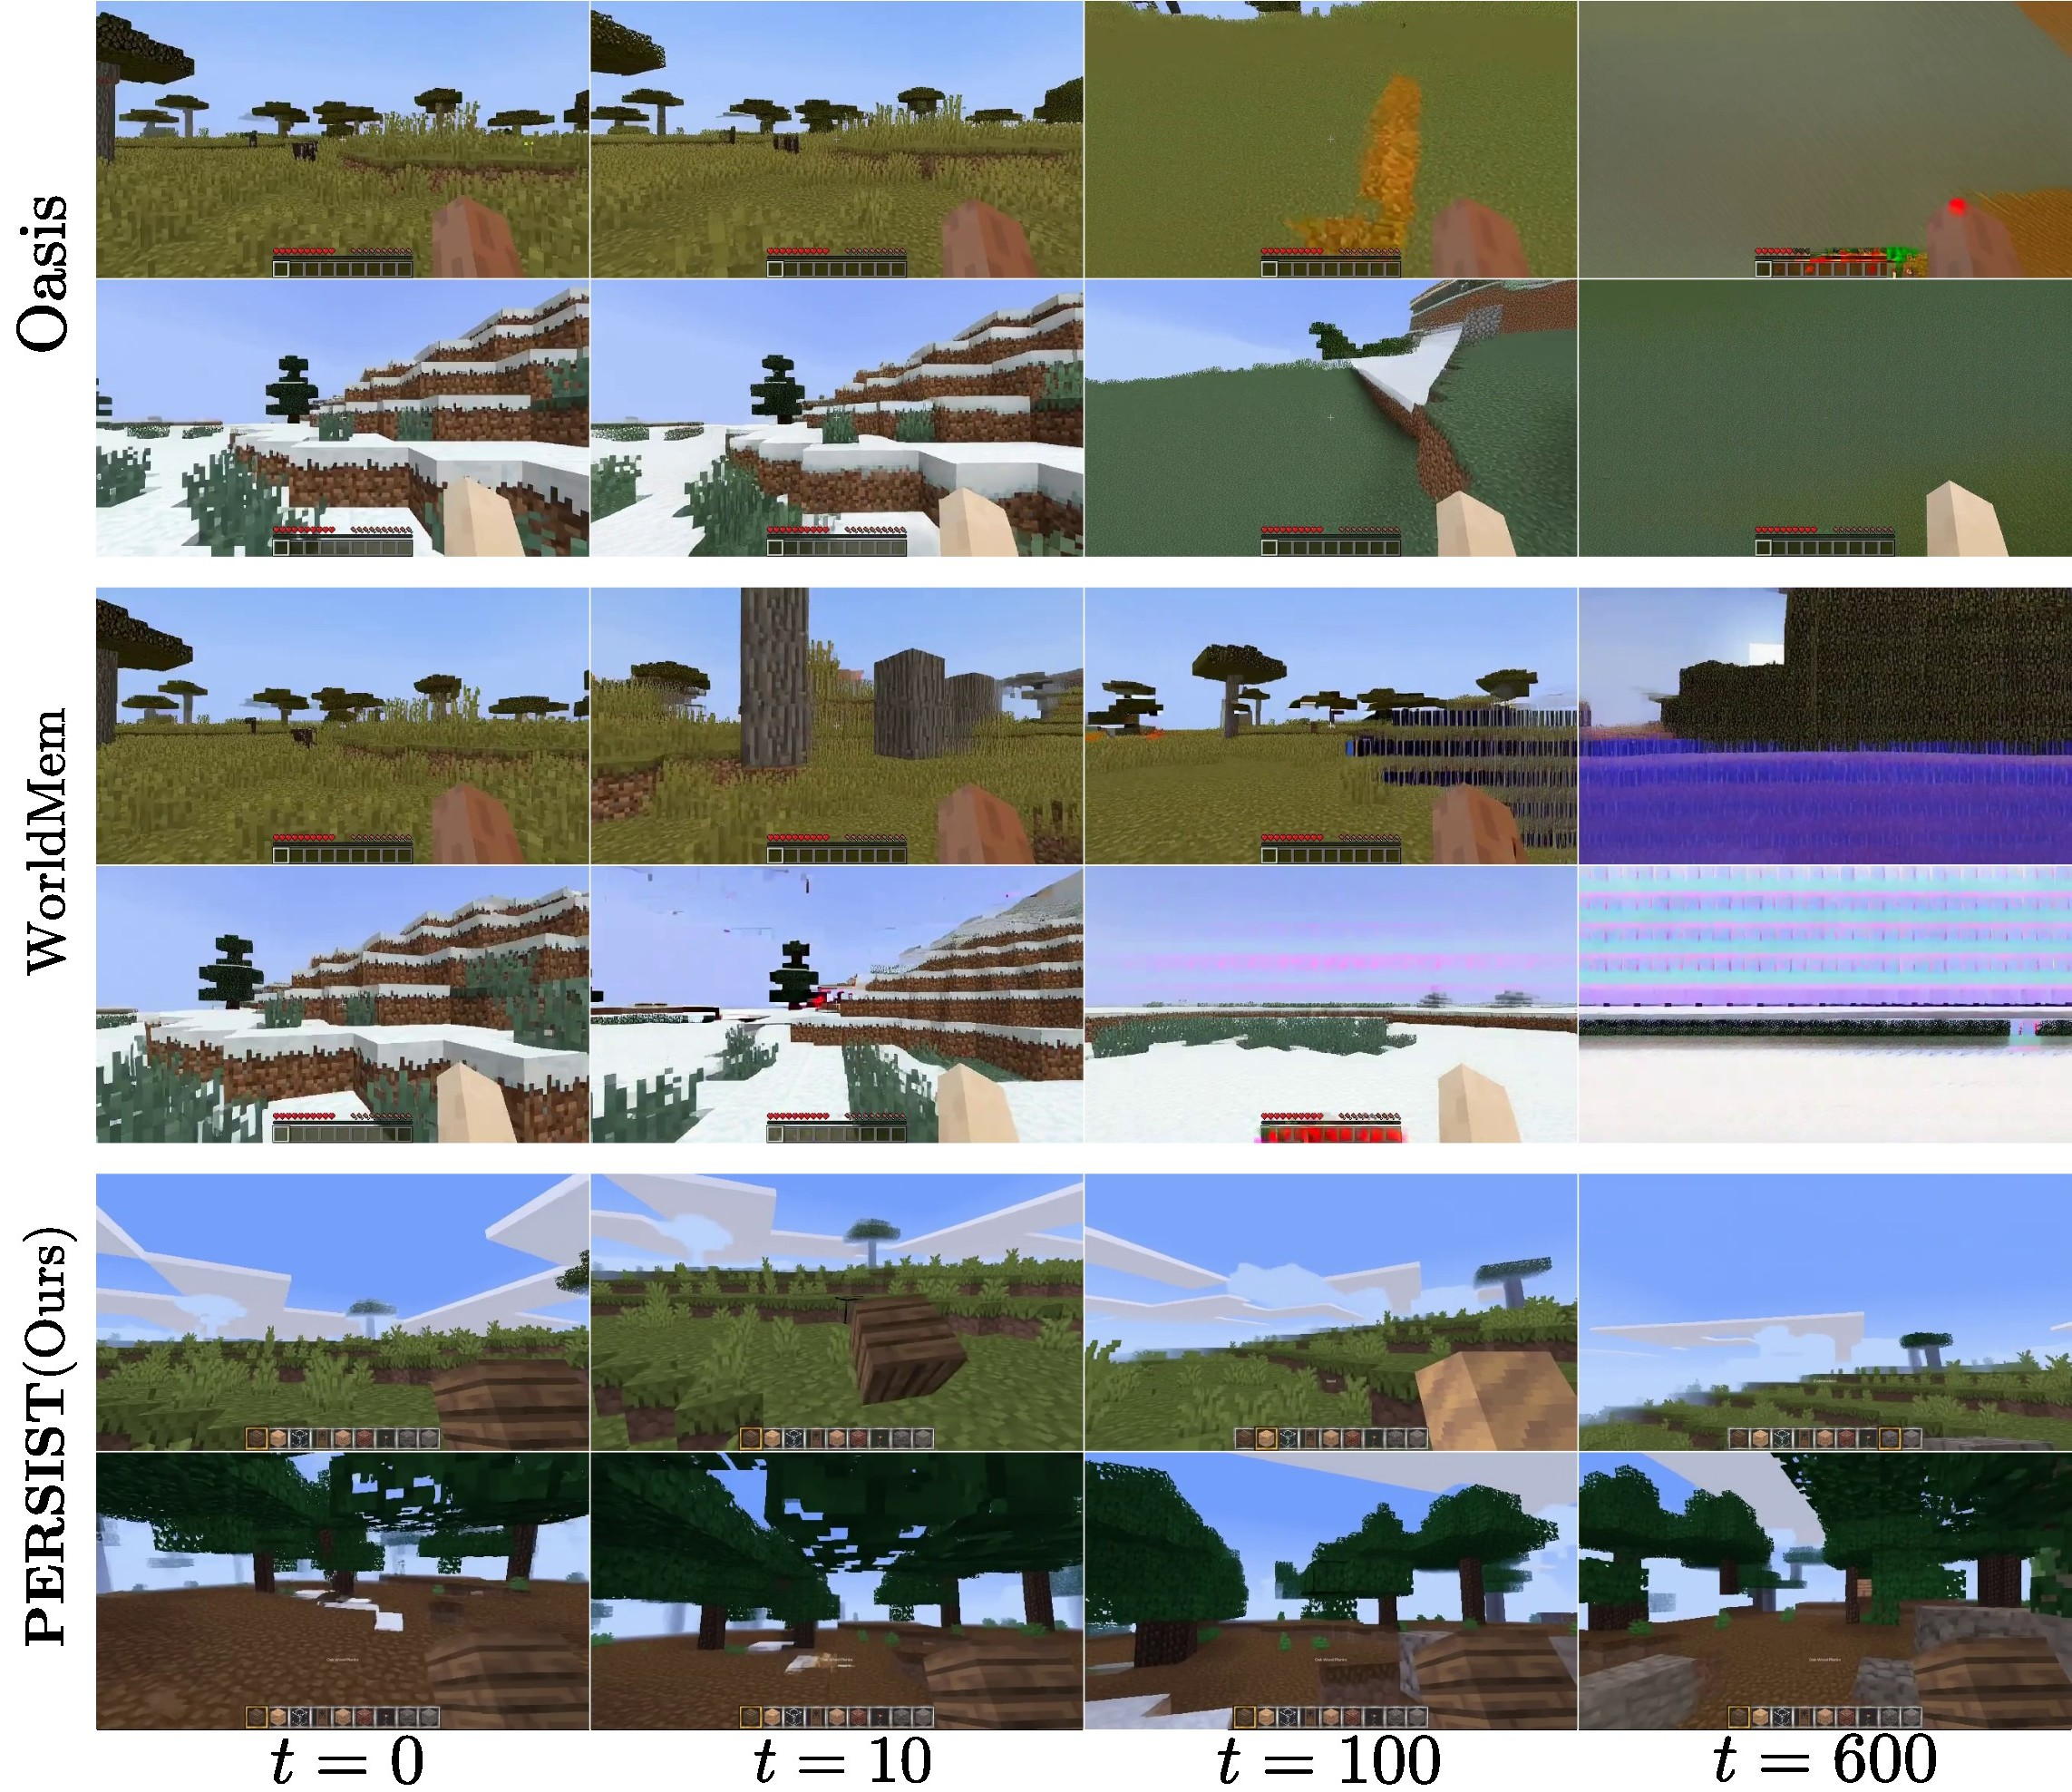
\includegraphics[width=0.8\linewidth]{figs/compare.jpg}}
    \caption{\DIFaddFL{Video frames generated over 600 timestep episodes by PERSIST (Ours), Oasis~\mbox{%DIFAUXCMD
\citep{decart2024oasis} }\hskip0pt%DIFAUXCMD
and WorldMem~\mbox{%DIFAUXCMD
\citep{xiao2025worldmem}}\hskip0pt%DIFAUXCMD
.}}
    \label{fig:rollout}
    \vspace{-0.5cm}
  \end{center}
\end{figure*}

% \DIFaddend \begin{table*}[t]
%   \centering
%   \caption{\DIFdelbeginFL \DIFdelFL{Comparison across evaluation modes}\DIFdelendFL \DIFaddbeginFL \DIFaddFL{FVD and mean user ratings (score range: 1-5) for videos generated from different PERSIST configurations and baselines}\DIFaddendFL . \DIFaddbeginFL \DIFaddFL{Bold numbers indicate the best performing methods. We find that every PERSIST configuration significantly outperforms baselines for all measured metrics. PERSIST-XL$+\vw_0$ is discussed in \mbox{%DIFAUXCMD
% \Cref{sec:new_app}}\hskip0pt%DIFAUXCMD
% .}\DIFaddendFL }
%     %\rowcolors{2}{gray!8}{white}
%     \DIFaddbeginFL \setlength{\tabcolsep}{4pt} %DIF >  default is 6pt
%     \DIFaddendFL \begin{tabular}{lccccc}
%     \toprule
%     Method & FVD\DIFaddbeginFL \DIFaddFL{$\downarrow$ }\DIFaddendFL & \DIFdelbeginFL \DIFdelFL{Visual Fidelity }\DIFdelendFL \DIFaddbeginFL \DIFaddFL{Per Frame Visual Fidelity$\uparrow$ }\DIFaddendFL & 3D Consistency\DIFaddbeginFL \DIFaddFL{$\uparrow$ }\DIFaddendFL & Temporal Consistency\DIFaddbeginFL \DIFaddFL{$\uparrow$ }\DIFaddendFL & Overall Score\DIFaddbeginFL \DIFaddFL{$\uparrow$ }\DIFaddendFL \\
%     \midrule
%     \DIFdelbeginFL \DIFdelFL{PERSIST-Base }\DIFdelendFL %DIF >  \addlinespace[-0.3em]
%     \midrule
%     \DIFaddFL{Oasis }\DIFaddendFL & \DIFdelbeginFL \DIFdelFL{209 }\DIFdelendFL \DIFaddbeginFL \DIFaddFL{706 }\DIFaddendFL & \DIFdelbeginFL \DIFdelFL{2.5 }\DIFdelendFL \DIFaddbeginFL \DIFaddFL{2.1 }\DIFaddendFL $\pm$ \DIFdelbeginFL \DIFdelFL{0.18 }\DIFdelendFL \DIFaddbeginFL \DIFaddFL{0.1 }\DIFaddendFL & \DIFdelbeginFL \DIFdelFL{2.6 }\DIFdelendFL \DIFaddbeginFL \DIFaddFL{1.9 }\DIFaddendFL $\pm$ \DIFdelbeginFL \DIFdelFL{0.19 }\DIFdelendFL \DIFaddbeginFL \DIFaddFL{0.1 }\DIFaddendFL & \DIFdelbeginFL \DIFdelFL{2.6 }\DIFdelendFL \DIFaddbeginFL \DIFaddFL{1.8 }\DIFaddendFL $\pm$ \DIFdelbeginFL \DIFdelFL{0.2 }\DIFdelendFL \DIFaddbeginFL \DIFaddFL{0.1 }\DIFaddendFL & \DIFdelbeginFL \DIFdelFL{2.6 }\DIFdelendFL \DIFaddbeginFL \DIFaddFL{1.9 }\DIFaddendFL $\pm$ \DIFdelbeginFL \DIFdelFL{0.18 }\DIFdelendFL \DIFaddbeginFL \DIFaddFL{0.1 }\DIFaddendFL \\
%     \DIFdelbeginFL \DIFdelFL{PERSIST-XL }\DIFdelendFL \DIFaddbeginFL \DIFaddFL{WorldMem }\DIFaddendFL & \DIFdelbeginFL \DIFdelFL{181 }\DIFdelendFL \DIFaddbeginFL \DIFaddFL{596 }\DIFaddendFL & \DIFdelbeginFL \textbf{\DIFdelFL{2.8 $\pm$ 0.16}} %DIFAUXCMD
% \DIFdelendFL \DIFaddbeginFL \DIFaddFL{1.7 $\pm$ 0.09 }\DIFaddendFL & \DIFdelbeginFL \textbf{\DIFdelFL{2.8 $\pm$ 0.15}} %DIFAUXCMD
% \DIFdelendFL \DIFaddbeginFL \DIFaddFL{1.7 $\pm$ 0.09 }\DIFaddendFL & \DIFdelbeginFL \textbf{\DIFdelFL{2.9 $\pm$ 0.16}} %DIFAUXCMD
% \DIFdelendFL \DIFaddbeginFL \DIFaddFL{1.5 $\pm$ 0.08 }\DIFaddendFL & \DIFdelbeginFL \textbf{\DIFdelFL{2.9 $\pm$ 0.15}} %DIFAUXCMD
% \DIFdelendFL \DIFaddbeginFL \DIFaddFL{1.5 $\pm$ 0.07 }\DIFaddendFL \\
%     \DIFdelbeginFL \DIFdelFL{PERSIST-XL$+\vw_0$ }\DIFdelendFL %DIF >  \midrule
%     \DIFaddbeginFL \DIFaddFL{PERSIST-S }\DIFaddendFL & \DIFdelbeginFL \textbf{\DIFdelFL{116}} %DIFAUXCMD
% \DIFdelendFL \DIFaddbeginFL \DIFaddFL{209 }\DIFaddendFL & \textbf{\DIFdelbeginFL \DIFdelFL{2.9 }\DIFdelendFL \DIFaddbeginFL \DIFaddFL{2.8 }\DIFaddendFL $\pm$ \DIFdelbeginFL \DIFdelFL{0.18}\DIFdelendFL \DIFaddbeginFL \DIFaddFL{0.1}\DIFaddendFL } & \textbf{2.7 $\pm$ \DIFdelbeginFL \DIFdelFL{0.23}\DIFdelendFL \DIFaddbeginFL \DIFaddFL{0.1}\DIFaddendFL } & \textbf{\DIFdelbeginFL \DIFdelFL{2.7 }\DIFdelendFL \DIFaddbeginFL \DIFaddFL{2.5 }\DIFaddendFL $\pm$ \DIFdelbeginFL \DIFdelFL{0.26}\DIFdelendFL \DIFaddbeginFL \DIFaddFL{0.1}\DIFaddendFL } & \textbf{\DIFdelbeginFL \DIFdelFL{2.8 }\DIFdelendFL \DIFaddbeginFL \DIFaddFL{2.6 }\DIFaddendFL $\pm$ \DIFdelbeginFL \DIFdelFL{0.22}\DIFdelendFL \DIFaddbeginFL \DIFaddFL{0.09}\DIFaddendFL } \\
%     \DIFdelbeginFL \DIFdelFL{Oasis }\DIFdelendFL \DIFaddbeginFL \DIFaddFL{PERSIST-XL }\DIFaddendFL & \DIFdelbeginFL \DIFdelFL{706 }\DIFdelendFL \DIFaddbeginFL \textbf{\DIFaddFL{181}} \DIFaddendFL & \DIFdelbeginFL \DIFdelFL{2.2 $\pm$ 0.15 }\DIFdelendFL \DIFaddbeginFL \textbf{\DIFaddFL{2.8 $\pm$ 0.09}} \DIFaddendFL & \DIFdelbeginFL \DIFdelFL{2.0 }\DIFdelendFL \DIFaddbeginFL \DIFaddFL{2.5 }\DIFaddendFL $\pm$ \DIFdelbeginFL \DIFdelFL{0.16 }\DIFdelendFL \DIFaddbeginFL \DIFaddFL{0.09 }\DIFaddendFL & \DIFdelbeginFL \DIFdelFL{1.9 $\pm$ 0.16 }\DIFdelendFL \DIFaddbeginFL \textbf{\DIFaddFL{2.5 $\pm$ 0.09}} \DIFaddendFL & \DIFdelbeginFL \DIFdelFL{2.0 $\pm$ 0.15 }\DIFdelendFL \DIFaddbeginFL \textbf{\DIFaddFL{2.6 $\pm$ 0.08}} \DIFaddendFL \\
%     \DIFdelbeginFL \DIFdelFL{WorldMem }\DIFdelendFL \midrule
%     \DIFaddFL{PERSIST-XL$+\vw_0$ }\DIFaddendFL & \DIFdelbeginFL \DIFdelFL{596 }\DIFdelendFL \DIFaddbeginFL \DIFaddFL{116 }\DIFaddendFL & \DIFdelbeginFL \DIFdelFL{1.7 }\DIFdelendFL \DIFaddbeginFL \DIFaddFL{3.2 }\DIFaddendFL $\pm$ \DIFdelbeginFL \DIFdelFL{0.12 }\DIFdelendFL \DIFaddbeginFL \DIFaddFL{0.1 }\DIFaddendFL & \DIFdelbeginFL \DIFdelFL{2.0 }\DIFdelendFL \DIFaddbeginFL \DIFaddFL{2.8 }\DIFaddendFL $\pm$ \DIFdelbeginFL \DIFdelFL{0.15 }\DIFdelendFL \DIFaddbeginFL \DIFaddFL{0.1 }\DIFaddendFL & \DIFdelbeginFL \DIFdelFL{1.8 }\DIFdelendFL \DIFaddbeginFL \DIFaddFL{2.8 }\DIFaddendFL $\pm$ \DIFdelbeginFL \DIFdelFL{0.15 }\DIFdelendFL \DIFaddbeginFL \DIFaddFL{0.1 }\DIFaddendFL & \DIFdelbeginFL \DIFdelFL{1.8 }\DIFdelendFL \DIFaddbeginFL \DIFaddFL{3.0 }\DIFaddendFL $\pm$ \DIFdelbeginFL \DIFdelFL{0.13 }\DIFdelendFL \DIFaddbeginFL \DIFaddFL{0.1 }\DIFaddendFL \\
%     \bottomrule
%     \end{tabular}
%   \label{tab:eval}
% \end{table*}

\DIFaddbegin \begin{figure*}[ht]
  \begin{center}
    \centerline{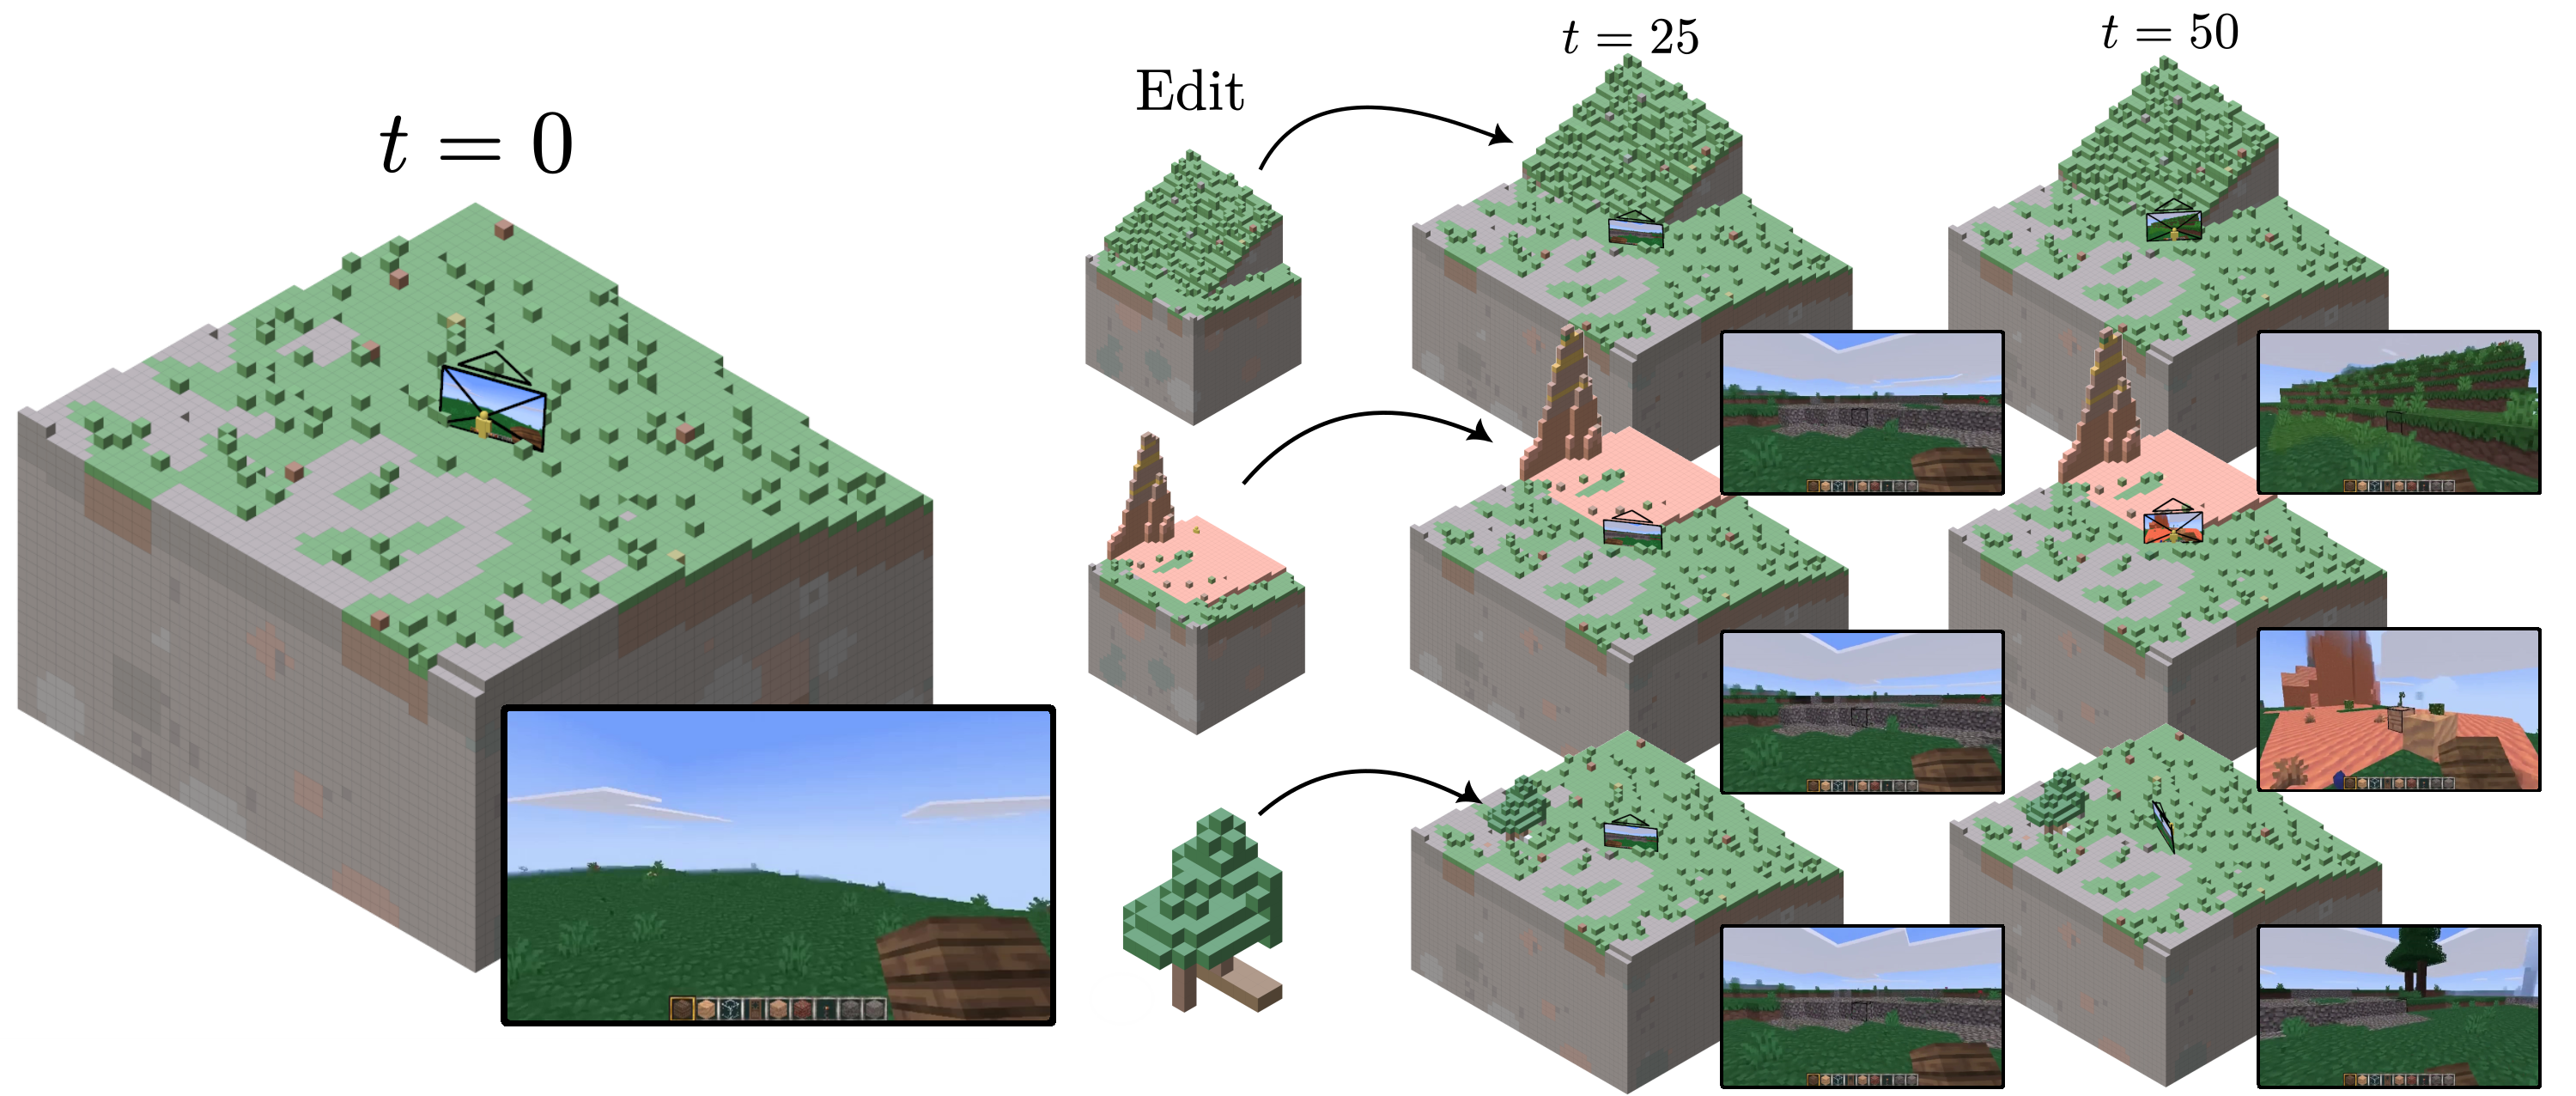
\includegraphics[width=0.9\linewidth]{figs/edits.png}}
    \caption{\DIFaddFL{PERSIST's explicit 3D representation allows us to edit the world-state during an episode, enabling intuitive fine grained control over generations. We demonstrate this above with both global edits to terrain and biome, as well as the placement of smaller assets such as trees.}}
    \label{fig:voxel-edits}
     \vspace{-0.2cm}
  \end{center}
\end{figure*}

\DIFaddend \subsection{Interactive Generation}

In this section, we assess our method's ability to generate interactive experiences that are both spatially and temporally consistent. We craft action policies specifically designed to make the agent explore its environment while continually revisiting previously rendered locations at different times and from various viewpoints. %DIF <   \todo[inline]{Mention trajectory lengths? very long rollouts? Define trajectory archetypes here or in the results table?}
 We deploy these policies in Craftium to collect a dataset of 148 evaluation trajectories from game worlds that were held-out from the training set. Finally, we sample starting conditions $\langle \vo_0, \vc_0\rangle$ and action \DIFdelbegin \DIFdel{sequence $A$ }\DIFdelend \DIFaddbegin \DIFadd{sequences }\DIFaddend from the evaluation set to generate trajectories with PERSIST-S (featuring the \DIFdelbegin \DIFdel{3D-Small }\DIFdelend \DIFaddbegin \DIFadd{3D-S }\DIFaddend denoiser) and PERSIST-XL (featuring the 3D-XL denoiser).

% old baseline section with more baselines, to add back for rebuttals
% \textbf{Baselines.} We compare our approach against Oasis [ref] and MineWorld [ref], two approaches conditioning directly on a past pixel observation window, as well as WorldMem [ref] and MemoryForcing [ref] which incorporate key-frame retrieval from a memory bank of past pixel observations. As these methods were trained with Minecraft data, we collect a separate evaluation set in Minedojo [ref] using the same evaluation policies, in order to not induce any domain shift and we replicate the baselines' respective inference configurations. In the case of WorldMem and MemoryForcing, this includes initialising their memory bank with 200 ground truth cameras and pixel observations, and providing ground truth cameras alongside actions during inference.

\textbf{Baselines.} We compare our approach with Oasis~\citep{decart2024oasis} and WorldMem~\citep{xiao2025worldmemlongtermconsistentworld}, two interactive video generation methods employing the same DiT backbone as $\gP_\theta$, but \DIFdelbegin \DIFdel{directly conditioning generation on observations }\DIFdelend \DIFaddbegin \DIFadd{only conditioning on observations sampled }\DIFaddend from $O^{t-1}$.
Oasis conditions on the most recent $O^{t-1}_{t-K}$ observations, and can therefore also be viewed as an ablation of PERSIST in which the guidance provided by $W_{2D}$ is disabled.
WorldMem \DIFdelbegin \DIFdel{actively tracks cameras }\DIFdelend \DIFaddbegin \DIFadd{tracks camera states }\DIFaddend during generation, and \DIFdelbegin \DIFdel{retrieves frames from $O^{t-1}$ closely matching its current camera prediction to use as key-frames to guide generation}\DIFdelend \DIFaddbegin \DIFadd{guides generation by retrieving from the full history key-frames closely matching the current camera state}\DIFaddend .
As these methods were trained using Minecraft data, we collect a separate evaluation set in Minedojo~\citep{fan2022minedojo} to not induce domain shift, and we replicate their respective inference configurations.
In the case of WorldMem, this includes initialising the memory bank used to sample key-frames with 600 ground truth cameras and pixel observations.
This contrasts with PERSIST, which is initialised from a single initial frame $\langle \vo_0, \vc_0 \rangle$.

% \textbf{Qualitative analysis.} \todo[inline]{write once we get to look at rollouts. Highlight problems with baselines etc}

% placeholder for results:
% FVD oasis: 705.6
% FVD world mem: 595.7 
% FVD PERSIST-Small
% FVD PERSIST-XL
% FVD PERSIST-XL + W_0

% For appendix
% Self-FVD Minetest: 62.5
% Self-FVD Minedojo 44.7

\textbf{\DIFdelbegin \DIFdel{User study}\DIFdelend \DIFaddbegin \DIFadd{Evaluation}\DIFaddend .}
\DIFdelbegin \DIFdel{In addition, we conduct a user study consisting of 300 evaluation trials, in which users are asked to score videos on their }\DIFdelend \DIFaddbegin \DIFadd{We conduct an user study comprising over 800 rollout evaluations from 28 participants. Users rate each video on }\DIFaddend ``Per-Frame Visual Fidelity'', \DIFdelbegin \DIFdel{their }\DIFdelend ``3D Spatial Consistency'', and \DIFdelbegin \DIFdel{their }\DIFdelend ``Temporal Environment Stability and Consistency'' before assigning an overall score. We \DIFdelbegin \DIFdel{complement this study with computing }\DIFdelend \DIFaddbegin \DIFadd{additionally report }\DIFaddend the Frechet Video Distance (FVD)~\citep{unterthiner2018towards} between each method and its \DIFdelbegin \DIFdel{respective }\DIFdelend \DIFaddbegin \DIFadd{corresponding }\DIFaddend evaluation set. \DIFdelbegin \DIFdel{Supplementing the FVD with a user evaluation is of particular interest to us, as the FVD measures the distance between the generated and ground truth videos, but does not }\DIFdelend \DIFaddbegin \DIFadd{While the FVD captures distribution-level discrepancies, it has a bias to favour per-frame visual quality over temporal consistency \mbox{%DIFAUXCMD
\citep{ge2024content}}\hskip0pt%DIFAUXCMD
. In contrast, human ratings }\DIFaddend directly assess spatial and temporal \DIFdelbegin \DIFdel{consistency for individual episodes. %DIF < Each trial consists of a pair of videos sampled at random from a pool consisting of generations obtained from our approach, the baselines and both evaluation sets. \todo[inline]{describe results. Maybe a good way to remotivate FVD measurements if Overall Scores and/or Visual quality and 3D consistency scores align with quantitative rankings}
}%DIFDELCMD < 

%DIFDELCMD < %%%
\textbf{\DIFdel{Quantitative analysis.}} %DIFAUXCMD
\DIFdel{We report results in \mbox{%DIFAUXCMD
\Cref{tab:eval}}\hskip0pt%DIFAUXCMD
. Across all evaluated metrics, each PERSIST configuration significantly outperforms all baselines, demonstrating the robustness of our framework. Improvements are consistent across both spatial and temporal consistency metrics, indicating that explicitly modelling }\DIFdelend \DIFaddbegin \DIFadd{coherence within individual episodes, making the two complementary. Results are summarised in \mbox{%DIFAUXCMD
\Cref{tab:eval}}\hskip0pt%DIFAUXCMD
, with full methodological details in \mbox{%DIFAUXCMD
\Cref{app:data_met} }\hskip0pt%DIFAUXCMD
and extended results in \mbox{%DIFAUXCMD
\Cref{app:ext_user_study}}\hskip0pt%DIFAUXCMD
.
}

\DIFadd{Across all metrics, PERSIST configurations consistently outperform the baselines, highlighting the benefits of explicitly maintaining }\DIFaddend a persistent 3D environment state\DIFdelbegin \DIFdel{yields systematic gains rather than isolated metric-specific effects.  Among user-study metrics, the smallest performance gap with prior work occurs for }\DIFdelend \DIFaddbegin \DIFadd{.  Improvements in FVD and }\DIFaddend per-frame visual \DIFdelbegin \DIFdel{quality when compared against Oasis. This result aligns with our design intent: PERSIST primarily targets long-horizon spatial and temporal consistency rather than frame-level appearance. Nonetheless, improvements in reported visual fidelity are significant, suggesting that PERSIST reduces the occurrence of visual artifacts. Finally, }\DIFdelend \DIFaddbegin \DIFadd{fidelity further indicate that guidance from $\vw_{2D}$ enhances visual quality. Qualitative rollouts (\mbox{%DIFAUXCMD
\Cref{fig:rollout}}\hskip0pt%DIFAUXCMD
) corroborate these findings, particularly over long horizons.
}

\textbf{\DIFadd{Spatial resolution of $\gW_\theta$.}} \DIFadd{While }\DIFaddend PERSIST-XL \DIFdelbegin \DIFdel{variants are scored consistently higher than }\DIFdelend \DIFaddbegin \DIFadd{achieves a lower FVD than PERSIST-S, we find that }\DIFaddend the \DIFdelbegin \DIFdel{PERSIST-Base configuration across all metrics, confirming that scaling the number of }\DIFdelend \DIFaddbegin \DIFadd{two configurations perform similarly in terms of average user ratings and during head-to-head comparisons (see \mbox{%DIFAUXCMD
\Cref{app:ext_user_study}}\hskip0pt%DIFAUXCMD
). This suggests that the effectiveness of the }\DIFaddend 3D \DIFdelbegin \DIFdel{spatial tokens }\DIFdelend \DIFaddbegin \DIFadd{representation is robust to reductions in the spatial resolution }\DIFaddend of $\gW_\theta$\DIFdelbegin \DIFdel{translates directly into improved world modelling performance}\DIFdelend .

%DIF > todo Add this again if head to head comparison is good. indicating that increasing the capacity of the 3D representation translates directly into stronger world modelling performance
\DIFaddbegin 

\DIFaddend % Notes on eval set:
% - describe eval set, make distinction between two type of trajectories: 
%        - Orbit: specifically designed to challenge spatial +  temporal consistency (spatial: viewing object/scenes from different view points, temporal: revisiting already explored locations/views)
%        - Free-Play: Agent perform randomised actions in the environment
%        - Exploration: Actions are aimed to cover a large distance (more timesteps, agent moves forward/backward and spins on itself periodically)


% Notes on Baselines:
% - describe baselines and highlight inherent limitations: e.g. Oasis/Mineworld have no memory mechanism (but Oasis uses 2x temporal context window as our models). WorldMem/MemoryForcing require hundred of GT frame to be warm-started at inference.
% - mention a separate eval set is collected in MineDojo to not induce domain shift for baselines.
% - mention our training set if much smaller than VPT training set (check size but I think 10-100x smaller

\subsection{New Applications and Emerging Capabilities}\DIFaddbegin \label{sec:new_app}
\DIFaddend 

\DIFaddbegin \begin{figure*}[ht]
  \begin{center}
    \centerline{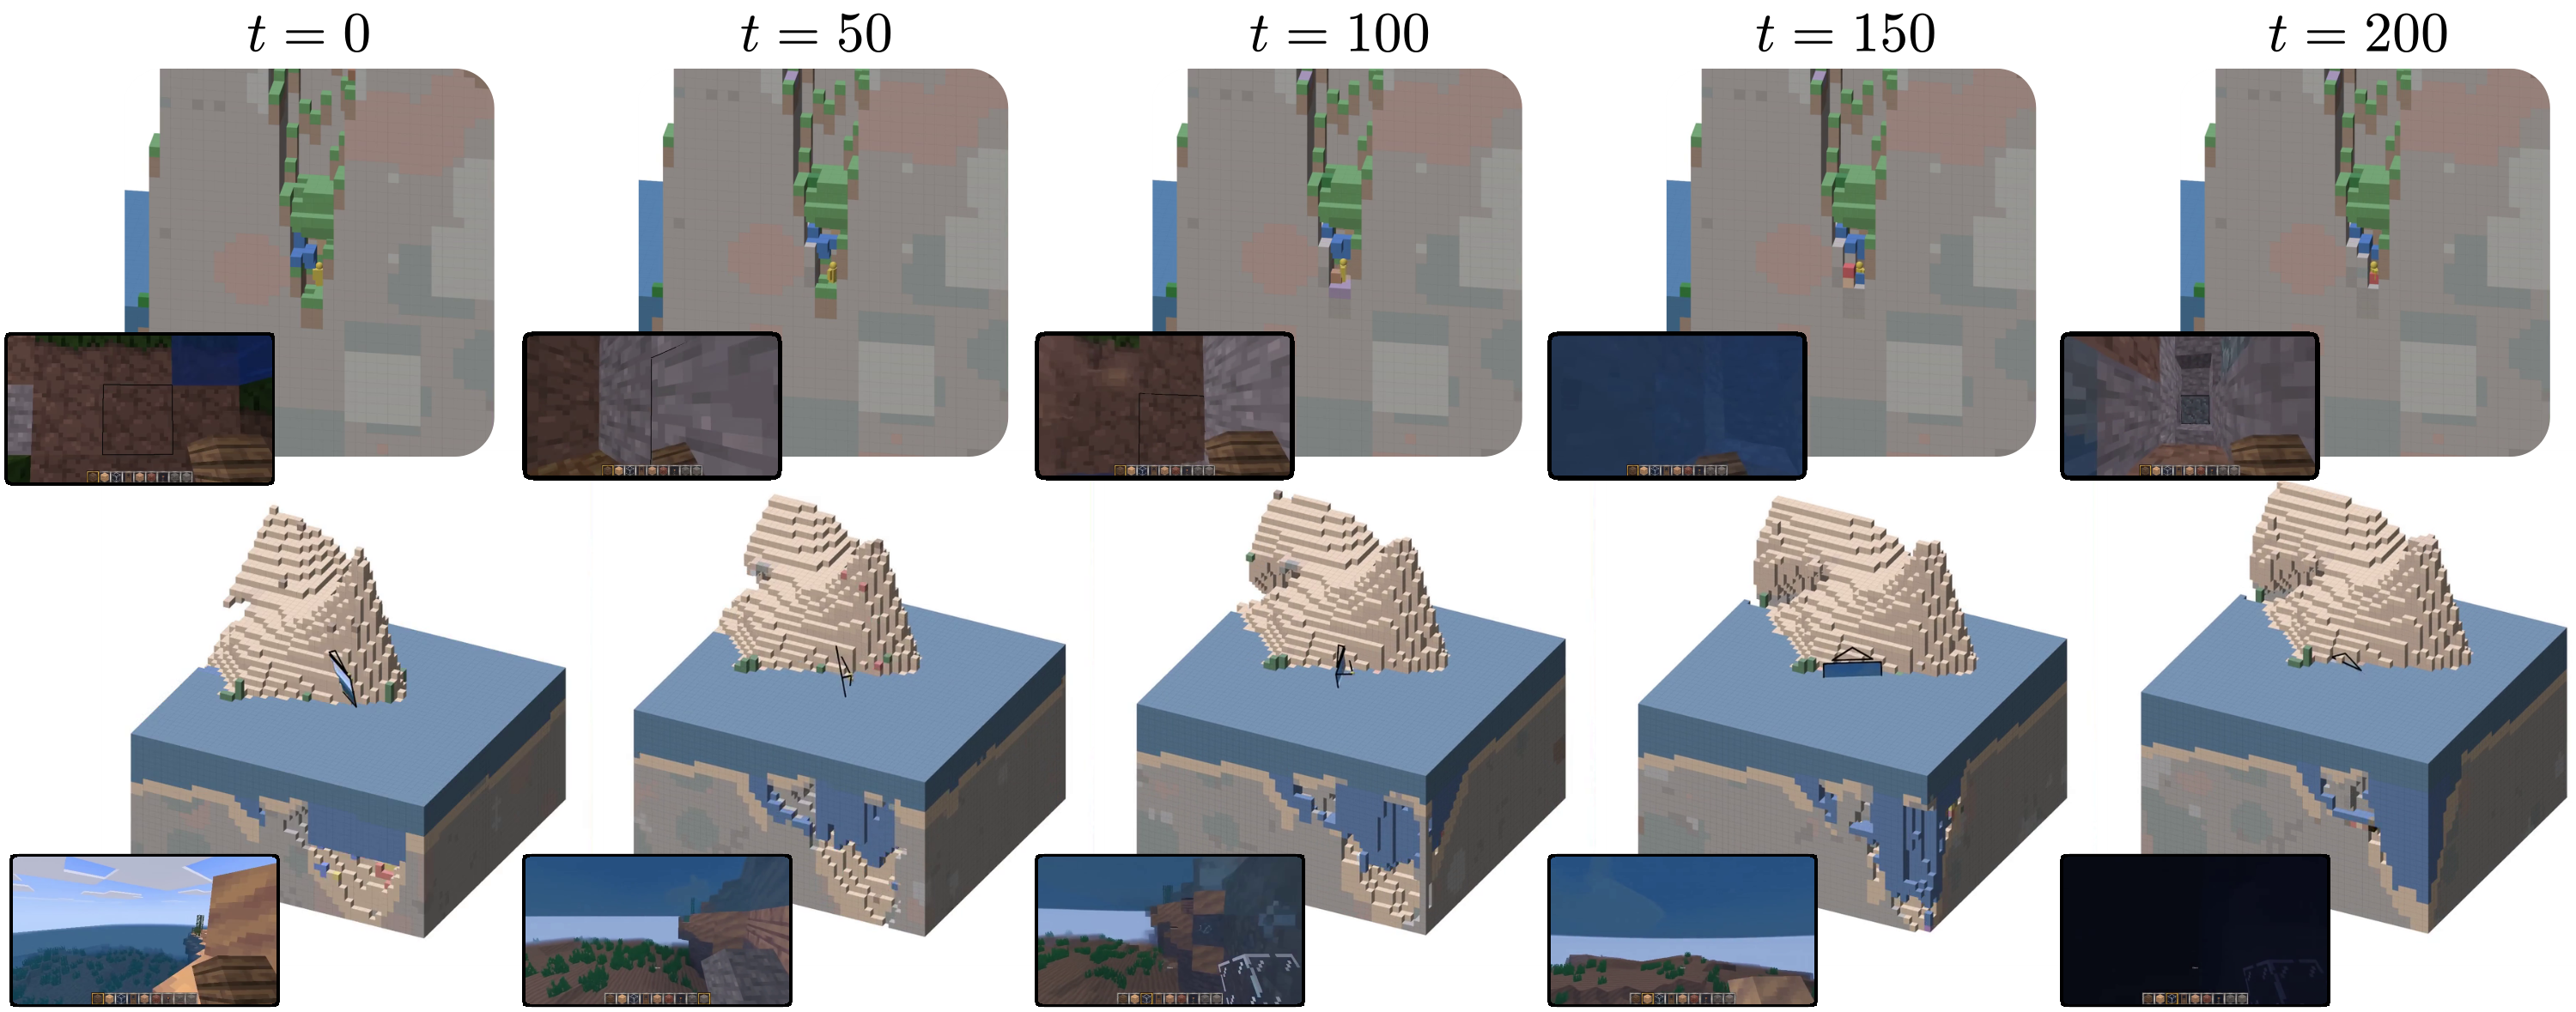
\includegraphics[width=\linewidth]{figs/dynamic.png}}
    \caption{\DIFaddFL{PERSIST maintains a dynamic 3D state that evolves even when unobserved (bottom: a cave filling with water), allowing off-screen events to produce on-screen effects (top: water flowing onto the player at $t=150$).}}
    \label{fig:dynamic}
     \vspace{-0.2cm}
  \end{center}
\end{figure*}

\DIFaddend In addition to \DIFdelbegin \DIFdel{maintaining strong spatial and temporal consistency over experiences spanning hundreds of frames, we discover additional capabilities afforded by our }\DIFdelend \DIFaddbegin \DIFadd{its improvement to the quality and coherence of generated experiences, we find that PERSIST's }\DIFaddend 3D \DIFdelbegin \DIFdel{dynamic model}\DIFdelend \DIFaddbegin \DIFadd{representation confers a number of new capabilities}\DIFaddend .

%DIF < Todo: example
\textbf{\DIFdelbegin \DIFdel{Explicit }\DIFdelend 3D \DIFdelbegin \DIFdel{initialisation}\DIFdelend \DIFaddbegin \DIFadd{generation}\DIFaddend .} At \DIFdelbegin \DIFdel{the start of an episode, we may directly provide a custom $\vw_0$ to the generation pipeline, instead of having it generated by }\DIFdelend \DIFaddbegin \DIFadd{initialisation, it is essential for $\vw_0$ to capture the structure and semantics of the provided conditioning RGB observation. In \mbox{%DIFAUXCMD
\Cref{fig:w0_gen}}\hskip0pt%DIFAUXCMD
, we show that }\DIFaddend $\gW_\theta$ \DIFaddbegin \DIFadd{successfully generates plausible starting world frames, while also outpainting unseen regions differently from one episode to the next. This ability lets PERSIST generate environments that are both diverse and coherent, supporting a wide variety of interactive experiences.
}

%DIF > Todo: example
\textbf{\DIFadd{Explicit 3D initialisation.}} \DIFadd{By default, PERSIST initialises generation from starting condition $\langle \vo_0, \vc_0\rangle$, with the initial world-frame $\vw_0$ being inferred by the world dynamics model $\gW_\theta$}\DIFaddend . \DIFdelbegin \DIFdel{This explicit conditioning provides }\DIFdelend \DIFaddbegin \DIFadd{However PERSIST also supports $\vw_0$ being provided as a starting condition. This explicit 3D conditioning allows }\DIFaddend a greater degree of control over the generated experience than providing an image, as the full surroundings of the agent \DIFdelbegin \DIFdel{are directly specified.
We observe a marked improvement in FVD when comparing }\DIFdelend \DIFaddbegin \DIFadd{can be specified.
}


\DIFadd{To assess how effectively PERSIST can leverage explicit 3D conditioning, we evaluate a variant denoted }\DIFaddend PERSIST-XL+$\vw_0$\DIFdelbegin \DIFdel{with }\DIFdelend \DIFaddbegin \DIFadd{, where a ground-truth world-frame $\vw_0$ is provided at initialisation. }\DIFaddend PERSIST-XL\DIFaddbegin \DIFadd{+$\vw_0$ improves over PERSIST-XL in terms of FVD and human ratings }\DIFaddend (\Cref{tab:eval}), \DIFdelbegin \DIFdel{indicating PERSIST-XL+}\DIFdelend \DIFaddbegin \DIFadd{demonstrating that the model successfully incorporates the additional information contained within }\DIFaddend $\vw_0$\DIFdelbegin \DIFdel{is successfully conditioning and maintaining the ground-truth 3D information about the environment. Crucially, PERSIST-XL+$\vw_0$ and PERSIST-XL perform similarly in user-ratings, which strongly indicates that PERSIST-XL is capable of generating plausible and self-consistent environments without requiring 3D ground truth information at initialisation}\DIFdelend . %DIF >  COMMENTED BECAUSE NO LONGER TRUE WITH LARGER HUMAN STUDY Notably, PERSIST-XL and PERSIST-XL+$\vw_0$ achieve similar human ratings. Here, FVD gains primarily reflect how additional information about the environment's initial state brings closer alignment with the evaluation videos. However there is no perceptible impact to the consistency or the quality of individual experiences when this information is not available, as PERSIST successfully extrapolates from $\langle \vo_0, \vc_0\rangle$ to generate a coherent 3D environment.

%DIF <  \textbf{World edits mid-generation.} [ref GameNGen, WHAM] proposed to perform manual edits to the generated pixel frames before re-injecting them as context, as an alternative way of influencing the generated experience. Similarly, as we can extract $\vw_t$ at any point during generation, we obtain the capability of making precise 3D-edits to the world mid-episode. To do so, we pause generation after timestep $t$ and manually edit $\vw_t$ to obtain $\tilde{\vw}_t$. We then restart generation using $\{\tilde{\vw}_t, \vc_t, \vo_t, \va_t\}$ as the starting condition. We show a few examples of this in \Cref{fig:world-edits}.
\DIFaddbegin \textbf{\DIFadd{World edits mid-generation.}} \DIFadd{\mbox{%DIFAUXCMD
\citet{valevski2024diffusionmodelsrealtimegame} }\hskip0pt%DIFAUXCMD
and \mbox{%DIFAUXCMD
\citet{kanervisto2025world} }\hskip0pt%DIFAUXCMD
proposed to perform manual edits to generated pixel frames before re-injecting them as context, as an alternative way of controlling the generated experience. Similarly, as we can extract $\vw_t$ at any point during generation, we obtain the capability of making precise 3D-edits to the world mid-episode. To do so, we pause generation after timestep $t$ and manually edit $\vw_t$ to obtain $\tilde{\vw}_t$. We then restart generation using $\{\tilde{\vw}_t, \vc_t, \vo_t, \va_t\}$ as the starting condition. We show several edit examples in \mbox{%DIFAUXCMD
\Cref{fig:voxel-edits}}\hskip0pt%DIFAUXCMD
.
}\DIFaddend 

%DIF <  \textbf{Persistent world dynamics.} In \Cref{fig:waterfall}\todo{fig}, we show how PERSIST learns to model dynamic processes in the environment, such as a water falling on top of the player. Such environment dynamics remain actively modeled even while they are not rendered to screen space: a few seconds later, as the player revisits its prior location, the waterfall is present and is slowly flooding the area.
\DIFaddbegin \textbf{\DIFadd{Persistent world dynamics.}} \DIFadd{PERSIST learns to model environmental processes that evolve on their own. In \mbox{%DIFAUXCMD
\Cref{fig:dynamic} }\hskip0pt%DIFAUXCMD
we provide examples of environment changes occurring outside of the agent's view, sometimes giving rise to unexpected interactions, e.g. water flowing onto the agent from above.
}\DIFaddend 

%DIF > PERSIST continuously models dynamic processes in the environment, even while they are not being actively rendered to screen space. In \Cref{dynamic}, we observe a waterfall gradually flooding the area, causing some water to eventually appear in the player's view.
\DIFaddbegin 

\DIFaddend \section{Conclusion}

In this work, we introduced PERSIST, a world \DIFdelbegin \DIFdel{modeling framework that moves beyond pixel-based histories by explicitly modeling }\DIFdelend \DIFaddbegin \DIFadd{modelling framework that tracks }\DIFaddend the evolution of a persistent latent 3D state. Our results demonstrate that actively generating guidance frames from this 3D state substantially improves spatial memory, temporal coherence, and overall generation quality compared to \DIFdelbegin \DIFdel{AR approaches conditioning on a limited window of past pixel observations, or retrieving key frames from a memory bank. In addition, we show that explicitly tracking the }\DIFdelend \DIFaddbegin \DIFadd{conditioning on pixel-based histories. We show that tracking this }\DIFaddend 3D \DIFdelbegin \DIFdel{state of the world leads to novel ways of controlling generated experiences, by allowing to }\DIFdelend \DIFaddbegin \DIFadd{world state allows the model to capture environment dynamics occurring beyond the agent's view. Additionally, it lets users }\DIFaddend pre-specify, visualise\DIFaddbegin \DIFadd{, }\DIFaddend and modify the structure of generated environments\DIFaddbegin \DIFadd{, creating new ways of controlling generated experiences}\DIFaddend .

\DIFdelbegin \paragraph{\DIFdel{Current limitations.}} %DIFAUXCMD
\addtocounter{paragraph}{-1}%DIFAUXCMD
\DIFdel{While PERSIST yields substantial improvements in generation quality, temporal stability, and environmental coherence, human evaluators consistently assign higher scores to }\DIFdelend \DIFaddbegin \DIFadd{Despite these advances, PERSIST currently relies on }\DIFaddend ground-truth \DIFdelbegin \DIFdel{videos, with average ratings in the range of 4.0–4.3 across metrics and a lower variance. This gap highlights that accurately and robustly modelling complex }\DIFdelend 3D \DIFdelbegin \DIFdel{environments over extended interactions remains an open challenge. In our generated rollouts, we observe gradual degradation in visual quality and physical stability over time, occasionally manifesting as artifacts such as minor jittering or imperfect player–environment alignment (e.g., floating effects). We attribute these behaviours primarily to exposure bias: during inference, each component of the pipeline must condition on its own predictions as well as those of other models, despite having been trained independently using ground-truth targets. This mismatch leads to compounding errors and imperfect dynamics, although PERSIST remains substantially more stable than all evaluated baselines. We expect that incorporating an additional fine-tuning stage in which the full pipeline is trained on its own autoregressive rollouts would further improve long-horizon stability, as demonstrated in recent work~\mbox{%DIFAUXCMD
\citep{huang2025self}}\hskip0pt%DIFAUXCMD
. We leave an investigation of this direction to future work.
}%DIFDELCMD < 

%DIFDELCMD < %%%
\paragraph{\DIFdel{Future work.}} %DIFAUXCMD
\addtocounter{paragraph}{-1}%DIFAUXCMD
\DIFdel{PERSIST currently assumes access to ground-truth }\DIFdelend \DIFaddbegin \DIFadd{supervision during training, and faces challenges common to AR generation, such as error accumulation and memory constraints. We report examples of generation artifacts caused by error accumulation over the course of a 2000 steps episode in \mbox{%DIFAUXCMD
\Cref{fig:limitations}}\hskip0pt%DIFAUXCMD
. We believe these limitations outline a clear roadmap for future research involving persistent }\DIFaddend 3D \DIFdelbegin \DIFdel{information and camera poses during training , which restricts its applicability to settings where such information can be obtained, for instance from game engines, simulators, or datasets containing }\DIFdelend \DIFaddbegin \DIFadd{world states: in-the-wild training via synthetic }\DIFaddend 3D annotations \DIFdelbegin \DIFdel{~\mbox{%DIFAUXCMD
\citep{zhou2018stereo,Matterport3D,yeshwanth2023scannet++}}\hskip0pt%DIFAUXCMD
.
An important direction for future work is to relax this requirement by leveraging recent advances in }\DIFdelend \DIFaddbegin \DIFadd{obtained from }\DIFaddend 2D-to-3D foundation models~\citep{wang2025vggt,sam3dteam2025sam3d3dfyimages}\DIFdelbegin \DIFdel{to estimate world structure and camera parameters directly from pixel observations as a pre-processing step.
PERSIST presently tracks a fixed region of 3D space centered on the agent, causing information outside this region to be discarded as the agent moves through the environment.
Enabling dynamic loading and unloading of spatial chunks from }\DIFdelend \DIFaddbegin \DIFadd{, end-to-end post-training on generated rollouts to mitigate autoregressive drift~\mbox{%DIFAUXCMD
\citep{huang2025self}}\hskip0pt%DIFAUXCMD
, and access to unconstrained spatial memory via }\DIFaddend a 3D memory bank\DIFdelbegin \DIFdel{would provide a natural path toward scaling PERSIST to retain spatial information over arbitrarily large environments.
Finally, extending PERSIST to model multiple agents within a shared world-frame represents an exciting avenue for future work, opening the door to multi-agent interaction within coherent, persistent environments.
}\DIFdelend \DIFaddbegin \DIFadd{. We provide a detailed discussion of these directions in Appendix~\ref{app:limitations}.
}\DIFaddend 

\section*{Impact Statement}

This work advances the field of Machine Learning by improving the spatial and temporal consistency of generative world models.
While our research is primarily conducted within the simulated environment of Luanti, the underlying methodologies have potential applications in video games, digital twin simulation, and embodied AI navigation, where reliable 3D scene representation is critical.
We do not foresee any immediate negative societal consequences that require specific highlighting at this stage, as our model operates within a synthetic domain.

% In the unusual situation where you want a paper to appear in the
% references without citing it in the main text, use \nocite
% \nocite{langley00}

\bibliography{biblio}  
\bibliographystyle{icml2026}

%%%%%%%%%%%%%%%%%%%%%%%%%%%%%%%%%%%%%%%%%%%%%%%%%%%%%%%%%%%%%%%%%%%%%%%%%%%%%%%
%%%%%%%%%%%%%%%%%%%%%%%%%%%%%%%%%%%%%%%%%%%%%%%%%%%%%%%%%%%%%%%%%%%%%%%%%%%%%%%
% APPENDIX
%%%%%%%%%%%%%%%%%%%%%%%%%%%%%%%%%%%%%%%%%%%%%%%%%%%%%%%%%%%%%%%%%%%%%%%%%%%%%%%
%%%%%%%%%%%%%%%%%%%%%%%%%%%%%%%%%%%%%%%%%%%%%%%%%%%%%%%%%%%%%%%%%%%%%%%%%%%%%%%
\newpage
\appendix
\DIFaddbegin \crefalias{section}{appendix}
\DIFaddend \onecolumn
\DIFdelbegin \section{\DIFdel{Model hyperparameters.}}%DIFAUXCMD
\addtocounter{section}{-1}%DIFAUXCMD
%DIFDELCMD < \label{app:model}
%DIFDELCMD < %%%
\DIFdelend 

\DIFaddbegin \section{\DIFadd{Additional Implementation Details}}\label{app:implt}


\subsection{\DIFadd{Additional Model Details}}

\textbf{\DIFadd{2D VAE.}} \DIFadd{We employ a vision transformer architecture \mbox{%DIFAUXCMD
\cite{dosovitskiy2020image}}\hskip0pt%DIFAUXCMD
, using the open-source implementation of \mbox{%DIFAUXCMD
\cite{decart2024oasis}}\hskip0pt%DIFAUXCMD
. We train the VAE via an MSE reconstruction objective, alongside a KL divergence penalty coefficient of $1e-6$.
}

\textbf{\DIFadd{3D VAE.}} \DIFadd{We employ a 3D-ResNet architecture based on the implementation provided by \mbox{%DIFAUXCMD
\cite{xiang2024structured}}\hskip0pt%DIFAUXCMD
. We train the VAE via a cross-entropy loss to predict voxel class labels, alongside a KL divergence penalty coefficient of $1e-6$.
}

\textbf{\DIFadd{Differentiable Rasterizer.}} \DIFadd{For our projecting function $\mathcal{R}$, we leverage GPU-native triangle rasterization, by assigning voxel features to faces of a static voxel-grid mesh. Then, depth-peeling~\mbox{%DIFAUXCMD
\cite{bavoil2008order, nagy2003depth} }\hskip0pt%DIFAUXCMD
is applied during rasterization to produce a per-pixel, depth-ordered stack of 3D features $W_{2D}^{t} \in \mathbb{R}^{H \times W \times L \times C}$, where $L$ is the maximum number of layers. Since the mesh topology is fixed for a given resolution, we construct it once at initialisation, updating vertex attributes in-place to avoid redundant mesh construction.  
}

\subsection{\DIFadd{PERSIST and PERSIST$+w_0$ Inference Logic}}

% \begin{algorithm}[htb!]
% \centering
% \caption{\DIFadd{PERSIST inference logic.}}\label{alg:PERSIST}
% \begin{algorithmic}[1]
% \Input{Models $\gW_\theta$, $\gC_\theta$, $\gP_\theta$, 2D-VAE, 3D-VAE, \\ Model context window sizes $K_{\gW}$, $K_{\gC}$, $K_{\gP}$, \\ 
% Renderer $\gR$, \\
% Initial conditions $o_\text{init}$, $c_\text{init}$, \\
% Episode Length $T$, \\
% Agent.}
% \State{$a_\text{init}\leftarrow \text{NO-OP}$} \Comment{Pipeline is always initialised using a NO-OP action.}
% \State{$\bar{o}_0 \leftarrow \text{2D-VAE.encode}(o_\text{init})$}
% \State{$\bar{w}_0 \leftarrow \gW_\theta (a_\text{init}, c_\text{init}, \bar{o}_0)$}
% \State{$w_0 \leftarrow \text{3D-VAE.decode}(\bar{w}_0)$}
% \State{$w_{{2D}_0} \leftarrow \gR(w_0,c_\text{init})$}
% \State{$\bar{o}_0 \leftarrow \gP (w_{{2D}_0}, a_\text{init}$)} \Comment{Regenerating the starting observation from $w_0$ guarantees alignment between $w_0$ and $o_0$.}
% \State{$o_0 \leftarrow \text{2D-VAE.decode}(\bar{o}_0)$}
% \State{Initialise rollout buffers $\{A,C,O,\bar{O},W,\bar{W},W_{2D}\}$ with $a_\text{init},c_\text{init},o_0,\bar{o}_0,w_0,\bar{w}_0,w_{{2D}_0}$}
% \For{$t$ in $1,\dots,T$}
% \State{Append to $A$: $a_t \leftarrow \text{Agent}(o_{t-1})$}
% \State{Append to $\bar{W}$: $\bar{w}_t \leftarrow \gW_\theta(\bar{W}^{t-1}_{t-K_\gW}, A^t_{t-K_\gW}, C^{t-1}_{t-K_\gW-1}, \bar{O}^{t-1}_{t-K_\gW-1})$}
% \State{Append to $W$: $w_t \leftarrow \text{3D-VAE.decode}(\bar{w}_t)$}
% \State{Append to $C$: $c_t \leftarrow \gC_\theta (C^{t-1}_{t-1-K_\gC}, W^t_{t-K_\gC}, A^t_{t-K_\gC})$}
% \State{Append to $W_{2D}$: $w_{{2D}_t} \leftarrow \gR(w_t,c_t)$}
% \State{Append to $\bar{O}$: $\bar{o}_t \leftarrow \gP_\theta ({W_{2D}}_{t-K_\gP}^{t}, A^t_{t-K_\gP}, \bar{O}^{t-1}_{t-K_\gP})$}
% \State{Append to $O$: $o_t \leftarrow \text{2D-VAE.decode}(\bar{o}_t)$}
% \EndFor
% \end{algorithmic}
% \end{algorithm}


% \begin{algorithm}[htb!]
% \centering
% \caption{\DIFadd{PERSIST$+w_0$ inference logic. \textcolor{blue}{Changes to \Cref{alg:PERSIST} in blue.}}}\label{alg:PERSIST-w0}
% \begin{algorithmic}[1]
% \Input{Models $\gW_\theta$, $\gC_\theta$, $\gP_\theta$, 2D-VAE, 3D-VAE, \\ Model context window sizes $K_{\gW}$, $K_{\gC}$, $K_{\gP}$, \\ 
% Renderer $\gR$, \\
% Initial conditions $o_\text{init}$, $c_\text{init}$, \textcolor{blue}{$w_\text{init}$} \\
% Episode Length $T$, \\
% Agent.}
% \State{$a_\text{init}\leftarrow \text{NO-OP}$} \Comment{Pipeline is always initialised using a NO-OP action.}
% \State{$\bar{o}_0 \leftarrow \text{2D-VAE.encode}(o_\text{init})$}
% \ColorState{blue}{$\bar{w}_0 \leftarrow \text{3D-VAE.encode}(w_\text{init})$}
% \State{$w_{{2D}_0} \leftarrow \gR(\textcolor{blue}{w_\text{init}},c_\text{init})$}
% \ColorState{blue}{$\bar{o}_0 \leftarrow \text{2D-VAE.encode}(o_\text{init})$}
% \State{Initialise rollout buffers $\{A,C,O,\bar{O},W,\bar{W},W_{2D}\}$ with $a_\text{init},c_\text{init},\textcolor{blue}{o_\text{init}},\bar{o}_0,\textcolor{blue}{w_\text{init}},\bar{w}_0,w_{{2D}_0}$} \Comment{We can use $o_\text{init}$ directly as $o_\text{init}$ and $w_\text{init}$ are expected to be perfectly aligned.}
% \For{$t$ in $1,\dots,T$}
% \State{Append to $A$: $a_t \leftarrow \text{Agent}(o_{t-1})$}
% \State{Append to $\bar{W}$: $\bar{w}_t \leftarrow \gW_\theta(\bar{W}^{t-1}_{t-K_\gW}, A^t_{t-K_\gW}, C^{t-1}_{t-K_\gW-1}, \bar{O}^{t-1}_{t-K_\gW-1})$}
% \State{Append to $W$: $w_t \leftarrow \text{3D-VAE.decode}(\bar{w}_t)$}
% \State{Append to $C$: $c_t \leftarrow \gC_\theta (C^{t-1}_{t-1-K_\gC}, W^t_{t-K_\gC}, A^t_{t-K_\gC})$}
% \State{Append to $W_{2D}$: $w_{{2D}_t} \leftarrow \gR(w_t,c_t)$}
% \State{Append to $\bar{O}$: $\bar{o}_t \leftarrow \gP_\theta ({W_{2D}}_{t-K_\gP}^{t}, A^t_{t-K_\gP}, \bar{O}^{t-1}_{t-K_\gP})$}
% \State{Append to $O$: $o_t \leftarrow \text{2D-VAE.decode}(\bar{o}_t)$}
% \EndFor
% \end{algorithmic}
% \end{algorithm}

\clearpage

\subsection{\DIFadd{Model and Inference Hyperparameters}}

% \DIFaddend \begin{table}[htb!]
% \centering
% \DIFaddbeginFL \caption{\DIFaddFL{3D-VAE configuration.}}
% \DIFaddendFL \begin{tabular}{cc}\toprule  
% Parameter & Value \\
% \midrule
% input shape & [48, 48, 48, \DIFdelbeginFL \DIFdelFL{2415}\DIFdelendFL \DIFaddbeginFL \DIFaddFL{2138}\DIFaddendFL ] \\
% number of residual blocks & 2 \\
% middle channels & [32, 128, 512] \\
% \DIFdelbeginFL \DIFdelFL{latent channels }\DIFdelendFL \DIFaddbeginFL \DIFaddFL{$\bar{w}$ shape }\DIFaddendFL & \DIFaddbeginFL [\DIFaddFL{12, 12, 12, }\DIFaddendFL 48\DIFaddbeginFL ] \DIFaddendFL \\
% \DIFaddbeginFL \DIFaddFL{\# parameters }& \DIFaddFL{138M }\\
% \DIFaddendFL \bottomrule
% \end{tabular}
% \DIFdelbeginFL %DIFDELCMD < \caption{%
% {%DIFAUXCMD
% \DIFdelFL{W-VAE configurations.}}
% %DIFAUXCMD
% \DIFdelendFL \label{table:w-vae}
% \end{table}

% \begin{table}[htb!]
% \centering
% \DIFaddbeginFL \caption{\DIFaddFL{2D-VAE configuration.}}
% \DIFaddendFL \begin{tabular}{cc}\toprule  
% Parameter & Value \\
% \midrule
% input size & [360, 640, 3] \\
% patch size & 10 \\
% \DIFdelbeginFL \DIFdelFL{latent dimension }\DIFdelendFL \DIFaddbeginFL \DIFaddFL{$\bar{o}$ shape }\DIFaddendFL & \DIFaddbeginFL [\DIFaddFL{36, 64, }\DIFaddendFL 16\DIFaddbeginFL ] \DIFaddendFL \\
% encoder dimension & 1024 \\
% encoder depth & 6 \\
% encoder number of heads & 6 \\
% decoder dimension & 1024 \\
% decoder depth & 12 \\
% decoder number of heads & 16 \\
% \DIFaddbeginFL \DIFaddFL{\# parameters }& \DIFaddFL{227M }\\
% \DIFaddendFL \bottomrule
% \end{tabular}
% \DIFdelbeginFL %DIFDELCMD < \caption{%
% {%DIFAUXCMD
% \DIFdelFL{P-VAE configurations.}}
% %DIFAUXCMD
% \DIFdelendFL \label{table:p-vae}
% \end{table}

% \begin{table}[htb!]
% \centering
% \DIFaddbeginFL \caption{\DIFaddFL{Camera model configuration.}}
% \DIFaddendFL \begin{tabular}{cc}\toprule  
% Parameter & Value \\
% \midrule
% \DIFdelbeginFL \DIFdelFL{voxel shape }\DIFdelendFL \DIFaddbeginFL \DIFaddFL{rotation embedding channels }\DIFaddendFL & \DIFdelbeginFL %DIFDELCMD < [%%%
% \DIFdelFL{48, 16, 16, 16}%DIFDELCMD < ] %%%
% \DIFdelendFL \DIFaddbeginFL \DIFaddFL{256 }\DIFaddendFL \\
% \DIFdelbeginFL \DIFdelFL{hidden dimension }\DIFdelendFL \DIFaddbeginFL \DIFaddFL{translation embedding channels }\DIFaddendFL & \DIFdelbeginFL \DIFdelFL{128 }\DIFdelendFL \DIFaddbeginFL \DIFaddFL{256 }\DIFaddendFL \\
% \DIFdelbeginFL \DIFdelFL{latent dimension }%DIFDELCMD < & %%%
% \DIFdelFL{64 }%DIFDELCMD < \\
% %DIFDELCMD < %%%
% \DIFdelFL{pixel shape }%DIFDELCMD < & [%%%
% \DIFdelFL{16, 64, 36}%DIFDELCMD < ] \\
% %DIFDELCMD < %%%
% \DIFdelFL{hidden dimension }%DIFDELCMD < & %%%
% \DIFdelFL{64 }%DIFDELCMD < \\
% %DIFDELCMD < %%%
% \DIFdelFL{latent dimension }%DIFDELCMD < & %%%
% \DIFdelFL{32 }%DIFDELCMD < \\
% %DIFDELCMD < %%%
% \DIFdelFL{fusion hidden dimension }%DIFDELCMD < & %%%
% \DIFdelFL{512 }%DIFDELCMD < \\
% %DIFDELCMD < %%%
% \DIFdelFL{output dimension }%DIFDELCMD < & %%%
% \DIFdelFL{8 }%DIFDELCMD < \\
% %DIFDELCMD < %%%
% \DIFdelFL{context window }\DIFdelendFL \DIFaddbeginFL \DIFaddFL{hidden }\DIFaddendFL size & \DIFdelbeginFL \DIFdelFL{8 }\DIFdelendFL \DIFaddbeginFL \DIFaddFL{1024 }\DIFaddendFL \\
% \DIFdelbeginFL \DIFdelFL{camera context hidden dimension }\DIFdelendFL \DIFaddbeginFL \DIFaddFL{transformer blocks }\DIFaddendFL & \DIFdelbeginFL \DIFdelFL{256 }\DIFdelendFL \DIFaddbeginFL \DIFaddFL{12 }\DIFaddendFL \\
% \DIFdelbeginFL \DIFdelFL{camera context }\DIFdelendFL number of heads & \DIFdelbeginFL \DIFdelFL{8 }\DIFdelendFL \DIFaddbeginFL \DIFaddFL{12 }\DIFaddendFL \\
% \DIFdelbeginFL \DIFdelFL{camera context number of layers }\DIFdelendFL \DIFaddbeginFL \DIFaddFL{MLP ratio }\DIFaddendFL & \DIFdelbeginFL \DIFdelFL{3 }\DIFdelendFL \DIFaddbeginFL \DIFaddFL{4 }\DIFaddendFL \\
% \DIFdelbeginFL \DIFdelFL{action dimension }\DIFdelendFL \DIFaddbeginFL \DIFaddFL{context window size }\DIFaddendFL & \DIFdelbeginFL \DIFdelFL{23 }%DIFDELCMD < \\
% %DIFDELCMD < %%%
% \DIFdelFL{action context hidden dimension }%DIFDELCMD < & %%%
% \DIFdelFL{256 }%DIFDELCMD < \\
% %DIFDELCMD < %%%
% \DIFdelFL{action context number of heads }%DIFDELCMD < & %%%
% \DIFdelendFL 8 \\
% \DIFdelbeginFL \DIFdelFL{action context number of layers }\DIFdelendFL \DIFaddbeginFL \DIFaddFL{\# parameters }\DIFaddendFL & \DIFdelbeginFL \DIFdelFL{3 }\DIFdelendFL \DIFaddbeginFL \DIFaddFL{234M }\DIFaddendFL \\
% \bottomrule
% \end{tabular}
% \DIFdelbeginFL %DIFDELCMD < \caption{%
% {%DIFAUXCMD
% \DIFdelFL{Camera model configurations.}}
% %DIFAUXCMD
% \DIFdelendFL \label{table:cam-model}
% \end{table}

% \begin{table}[htb!]
% \centering
% \DIFaddbeginFL \caption{\DIFaddFL{World denoiser hyperparameters (3D-S configuration). The XL configuration uses patch size=1 and has the same number of learned parameters.}}
% \DIFaddendFL \begin{tabular}{cc}\toprule  
% Parameter & Value \\
% \midrule
% input shape & [\DIFdelbeginFL \DIFdelFL{16, 16, 16}\DIFdelendFL \DIFaddbeginFL \DIFaddFL{12, 12, 12}\DIFaddendFL , 48] \\
% patch size & 2 \\
% hidden size & 1024 \\
% \DIFaddbeginFL \DIFaddFL{cross condition hidden size }& \DIFaddFL{1024 }\\
% \DIFaddendFL depth & 12 \\
% number of heads & 16 \\
% \DIFdelbeginFL \DIFdelFL{mlp }\DIFdelendFL \DIFaddbeginFL \DIFaddFL{MLP }\DIFaddendFL ratio & \DIFdelbeginFL \DIFdelFL{4.0 }\DIFdelendFL \DIFaddbeginFL \DIFaddFL{4 }\DIFaddendFL \\
% pixel condition \DIFdelbeginFL \DIFdelFL{shape }%DIFDELCMD < & %%%
% \DIFdelFL{(16, 36, 64) }%DIFDELCMD < \\
% %DIFDELCMD < %%%
% \DIFdelFL{pixel condition }\DIFdelendFL patch size & 2 \\
% \DIFdelbeginFL \DIFdelFL{cross condition hidden size }%DIFDELCMD < & %%%
% \DIFdelFL{1024 }%DIFDELCMD < \\
% %DIFDELCMD < %%%
% \DIFdelFL{action condition dimension }%DIFDELCMD < & %%%
% \DIFdelFL{23 }%DIFDELCMD < \\
% %DIFDELCMD < %%%
% \DIFdelFL{camera condition dimension }%DIFDELCMD < & %%%
% \DIFdelFL{8 }%DIFDELCMD < \\
% %DIFDELCMD < %%%
% \DIFdelendFL context window size & 8 \\
% \DIFaddbeginFL \DIFaddFL{\# parameters }& \DIFaddFL{686M }\\
% \DIFaddendFL \bottomrule
% \end{tabular}
% \DIFdelbeginFL %DIFDELCMD < \caption{%
% {%DIFAUXCMD
% \DIFdelFL{World denoiser configurations.}}
% %DIFAUXCMD
% \DIFdelendFL \label{table:world-denoiser}
% \end{table}

% \begin{table}[htb!]
% \centering
% \DIFaddbeginFL \caption{\DIFaddFL{Pixel denoiser configuration.}}
% \DIFaddendFL \begin{tabular}{cc}\toprule  
% Parameter & Value \\
% \midrule
% \DIFdelbeginFL \DIFdelFL{input }\DIFdelendFL \DIFaddbeginFL \DIFaddFL{$\bar{o}$ }\DIFaddendFL shape & [\DIFdelbeginFL \DIFdelFL{16, 32}\DIFdelendFL \DIFaddbeginFL \DIFaddFL{36, 64}\DIFaddendFL , 16] \\
% \DIFaddbeginFL \DIFaddFL{$\bar{o}$ embedder output channels }& \DIFaddFL{16 }\\
% \DIFaddendFL patch size & 2 \\
% hidden size & 1024 \\
% depth & 12 \\
% number of heads & 16 \\
% \DIFdelbeginFL \DIFdelFL{voxel dimension }\DIFdelendFL \DIFaddbeginFL \DIFaddFL{MLP ratio }\DIFaddendFL & \DIFdelbeginFL \DIFdelFL{48 }\DIFdelendFL \DIFaddbeginFL \DIFaddFL{4 }\DIFaddendFL \\
% \DIFaddbeginFL \DIFaddFL{$\tilde{w}_{2D}$ shape }& [\DIFaddFL{36, 64, 192, 32}] \\
% \DIFaddFL{${w}_{2D}$ embedder patch size }& \DIFaddFL{6 }\\
% \DIFaddFL{${w}_{2D}$ embedder stride }& \DIFaddFL{4 }\\
% \DIFaddFL{${w}_{2D}$ embedder output channels }& \DIFaddFL{752 }\\
% \DIFaddFL{context window size }& \DIFaddFL{16 }\\
% \DIFaddFL{\# parameters }& \DIFaddFL{460M }\\

% \DIFaddendFL \bottomrule
% \end{tabular}
% \DIFdelbeginFL %DIFDELCMD < \caption{%
% {%DIFAUXCMD
% \DIFdelFL{Pixel denoiser configurations.}}
% %DIFAUXCMD
% \DIFdelendFL \label{table:pixel-denoiser}
% \end{table}

% \DIFaddbegin \begin{table}[htb!]
% \centering
% \caption{\DIFaddFL{Flow matching sampler configurations at inference time.}}
% \begin{tabular}{cc}\toprule  
% \DIFaddFL{Parameter }& \DIFaddFL{Value }\\
% \midrule
% \DIFaddFL{minimum noise $\sigma_\text{min}$ }& \DIFaddFL{$1e-5$ }\\
% \DIFaddFL{denoising steps }& \DIFaddFL{20 }\\
% \DIFaddFL{denoising step scheduling function }& \DIFaddFL{$\tau^k = \frac{\eta k}{1 + (\eta-1)k} $ }\\
% \DIFaddFL{$\eta$ }& \DIFaddFL{3 }\\
% \DIFaddFL{noise level applied to context (past) frames $\tau_\text{ctx}$ }& \DIFaddFL{0.02 ($\gW_\theta$) / 0.1 ($\gP_\theta$) }\\

% \bottomrule
% \end{tabular}
% \label{table:samplers}
% \end{table}

% \begin{table}[htb!]
%   \centering
%   \caption{\DIFaddFL{Number of spatial and temporal tokens for different models.}}
%     %DIF > \rowcolors{2}{gray!8}{white}
%     \begin{tabular}{lcc}
%     \toprule
%     \DIFaddFL{Model }& \DIFaddFL{\# Temporal Tokens }& \DIFaddFL{\# Spatial Tokens }\\
%     \midrule
%      \DIFaddFL{$\gW_\theta$-S }& \DIFaddFL{8 }& \DIFaddFL{216 }\\
%      \DIFaddFL{$\gW_\theta$-XL }& \DIFaddFL{8 }& \DIFaddFL{1728 }\\
%      \DIFaddFL{$\gP_\theta$ }& \DIFaddFL{16 }& \DIFaddFL{576 }\\
%      \DIFaddFL{$\gC_\theta$ }& \DIFaddFL{8 }& \DIFaddFL{n/a }\\
%     \bottomrule
%     \end{tabular}
% \end{table}

\DIFaddend \clearpage
\DIFdelbegin \section{\DIFdel{Evaluation Data and User Study}}%DIFAUXCMD
\addtocounter{section}{-1}%DIFAUXCMD
%DIFDELCMD < \label{app:data}
%DIFDELCMD < %%%
\DIFdelend 

\DIFaddbegin \section{\DIFadd{Evaluation Methodology}}\label{app:data_met}

%DIF >  \subsection{Training data}
%DIF >  \todo[inline]{
%DIF >  \begin{enumerate}
%DIF >      \item What policy was used? Describe action groups
%DIF >      \item Mention how long it takes to collect dataset
%DIF >      \item Any other important details?
%DIF >  \end{enumerate}
%DIF >  }

\subsection{\DIFadd{Evaluation data}}

\DIFaddend As discussed in the main body, we curated evaluation datasets across four modes to assess agent \DIFdelbegin \DIFdel{behavior}\DIFdelend \DIFaddbegin \DIFadd{behaviour}\DIFaddend : \textit{Free Play}, \textit{Move Forward}, \textit{Move Backward}, and \textit{Orbit}.
These modes are designed to \DIFdelbegin \DIFdel{highlight explorative behaviors that demand high levels }\DIFdelend \DIFaddbegin \DIFadd{produce trajectories that require a high level }\DIFaddend of temporal and spatial consistency \DIFaddbegin \DIFadd{to be correctly simulated by the world model}\DIFaddend .

\begin{itemize}
    \item \textbf{Free Play:} \DIFdelbegin \DIFdel{The agent follows a predefined stochastic sampling rule to execute random actions, facilitating diverse environmental }\DIFdelend \DIFaddbegin \DIFadd{randomly samples action from a set of pre-defined sequences, facilitating }\DIFaddend exploration.
    \item \textbf{Move Forward/Backward:} The agent \DIFdelbegin \DIFdel{performs a directed linear translation (forward or backward) followed by a rotational ``look around'' maneuver to observe the }\DIFdelend \DIFaddbegin \DIFadd{moves forwards or backwards, periodically spinning on itself to observe its }\DIFaddend surroundings.
    \item \textbf{Orbit:} The agent \DIFdelbegin \DIFdel{adheres to a policy that maintains a constant radius while rotating around a fixed central coordinate}\DIFdelend \DIFaddbegin \DIFadd{follows a circular trajectory, while constantly adjusting its heading to look towards the centre of the circle}\DIFaddend .
\end{itemize}

\DIFaddbegin \DIFadd{We collect evaluation sets in MineDojo and Craftium following these policies. }\DIFaddend For inference with \DIFdelbegin \textit{\DIFdel{WorldMem}}%DIFAUXCMD
\DIFdelend \DIFaddbegin \DIFadd{WorldMem}\DIFaddend , we prepend 600 \DIFdelbegin \DIFdel{context frames , collected within }\textit{\DIFdel{MineDojo}}%DIFAUXCMD
\DIFdel{, to the }\DIFdelend \DIFaddbegin \DIFadd{ground truth frames to each }\DIFaddend evaluation sequence to \DIFdelbegin \DIFdel{provide necessary historical state information}\DIFdelend \DIFaddbegin \DIFadd{warm-start the memory bank}\DIFaddend .

\DIFaddbegin \subsection{\DIFadd{FVD computation}}

\DIFadd{To compute the FVD, we collect a total of 148 rollouts of 192 frames for each method, splitting collection evenly across all four evaluation sets. Videos are spliced into 16-frame clips, for a total of 1776 clips. We then compute the FVD from the latent features obtained by passing rollout and ground truth clips through a pretrained Inflated 3D ConvNet \mbox{%DIFAUXCMD
\citep{carreira2017quo}}\hskip0pt%DIFAUXCMD
.
}

\DIFaddend \subsection{User Study Protocol}\DIFaddbegin \label{app:method_user_study}
\DIFaddend The user study was deployed via a custom web interface (see Figure~\ref{fig:ui_screenshot}). Participants were tasked \DIFdelbegin \DIFdel{with performing side-by-side comparisons of video pairs and providing qualitative ratings.
    These individual }\DIFdelend \DIFaddbegin \DIFadd{of scoring videos according to the following metrics and instructions:
}\begin{itemize}
    \item \textbf{\DIFadd{Visual Fidelity.}} \DIFadd{Per-frame visual quality of the video. Deduct points for visual artifacts such as blurriness, color shifts, flickering, noise, or texture degradation.
    }\item \textbf{\DIFadd{3D Spatial Consistency.}} \DIFadd{Spatial consistency of the scene. Deduct points if objects deform, shift, or change appearance when viewed from different camera angles, or if the relative depth and spatial relationships between objects appear inconsistent as the player moves.
    }\item \textbf{\DIFadd{Temporal Environment Stability and Consistency.}} \DIFadd{Consistency of the environment over time. Deduct points if the scene changes unexpectedly, such as objects disappearing, reappearing, or changing structure when revisiting previously seen areas, or if the environment degrades or becomes unnaturally simplified over time.
    }\item \textbf{\DIFadd{Overall Quality Score.}} \DIFadd{Your subjective rating of the overall quality of the video, considering all factors above.
}\end{itemize}
\DIFadd{Ratings had the range of 1-5. Videos were presented to the user as pairs. Each pair depicted matching behaviour (free play, move forward, move backward, orbit) but different methods (baselines, PERSIST configurations, Minedojo or Craftium ground truth). Each individual user was asked to rate up to 50 videos. User }\DIFaddend assessments were subsequently aggregated to compute \DIFdelbegin \DIFdel{the final performance metrics}\DIFdelend \DIFaddbegin \DIFadd{average scores. We consider the first three evaluation trials for each participant to count as calibration, and we discard them from the study}\DIFaddend .

\begin{figure}[ht]
    \centering
    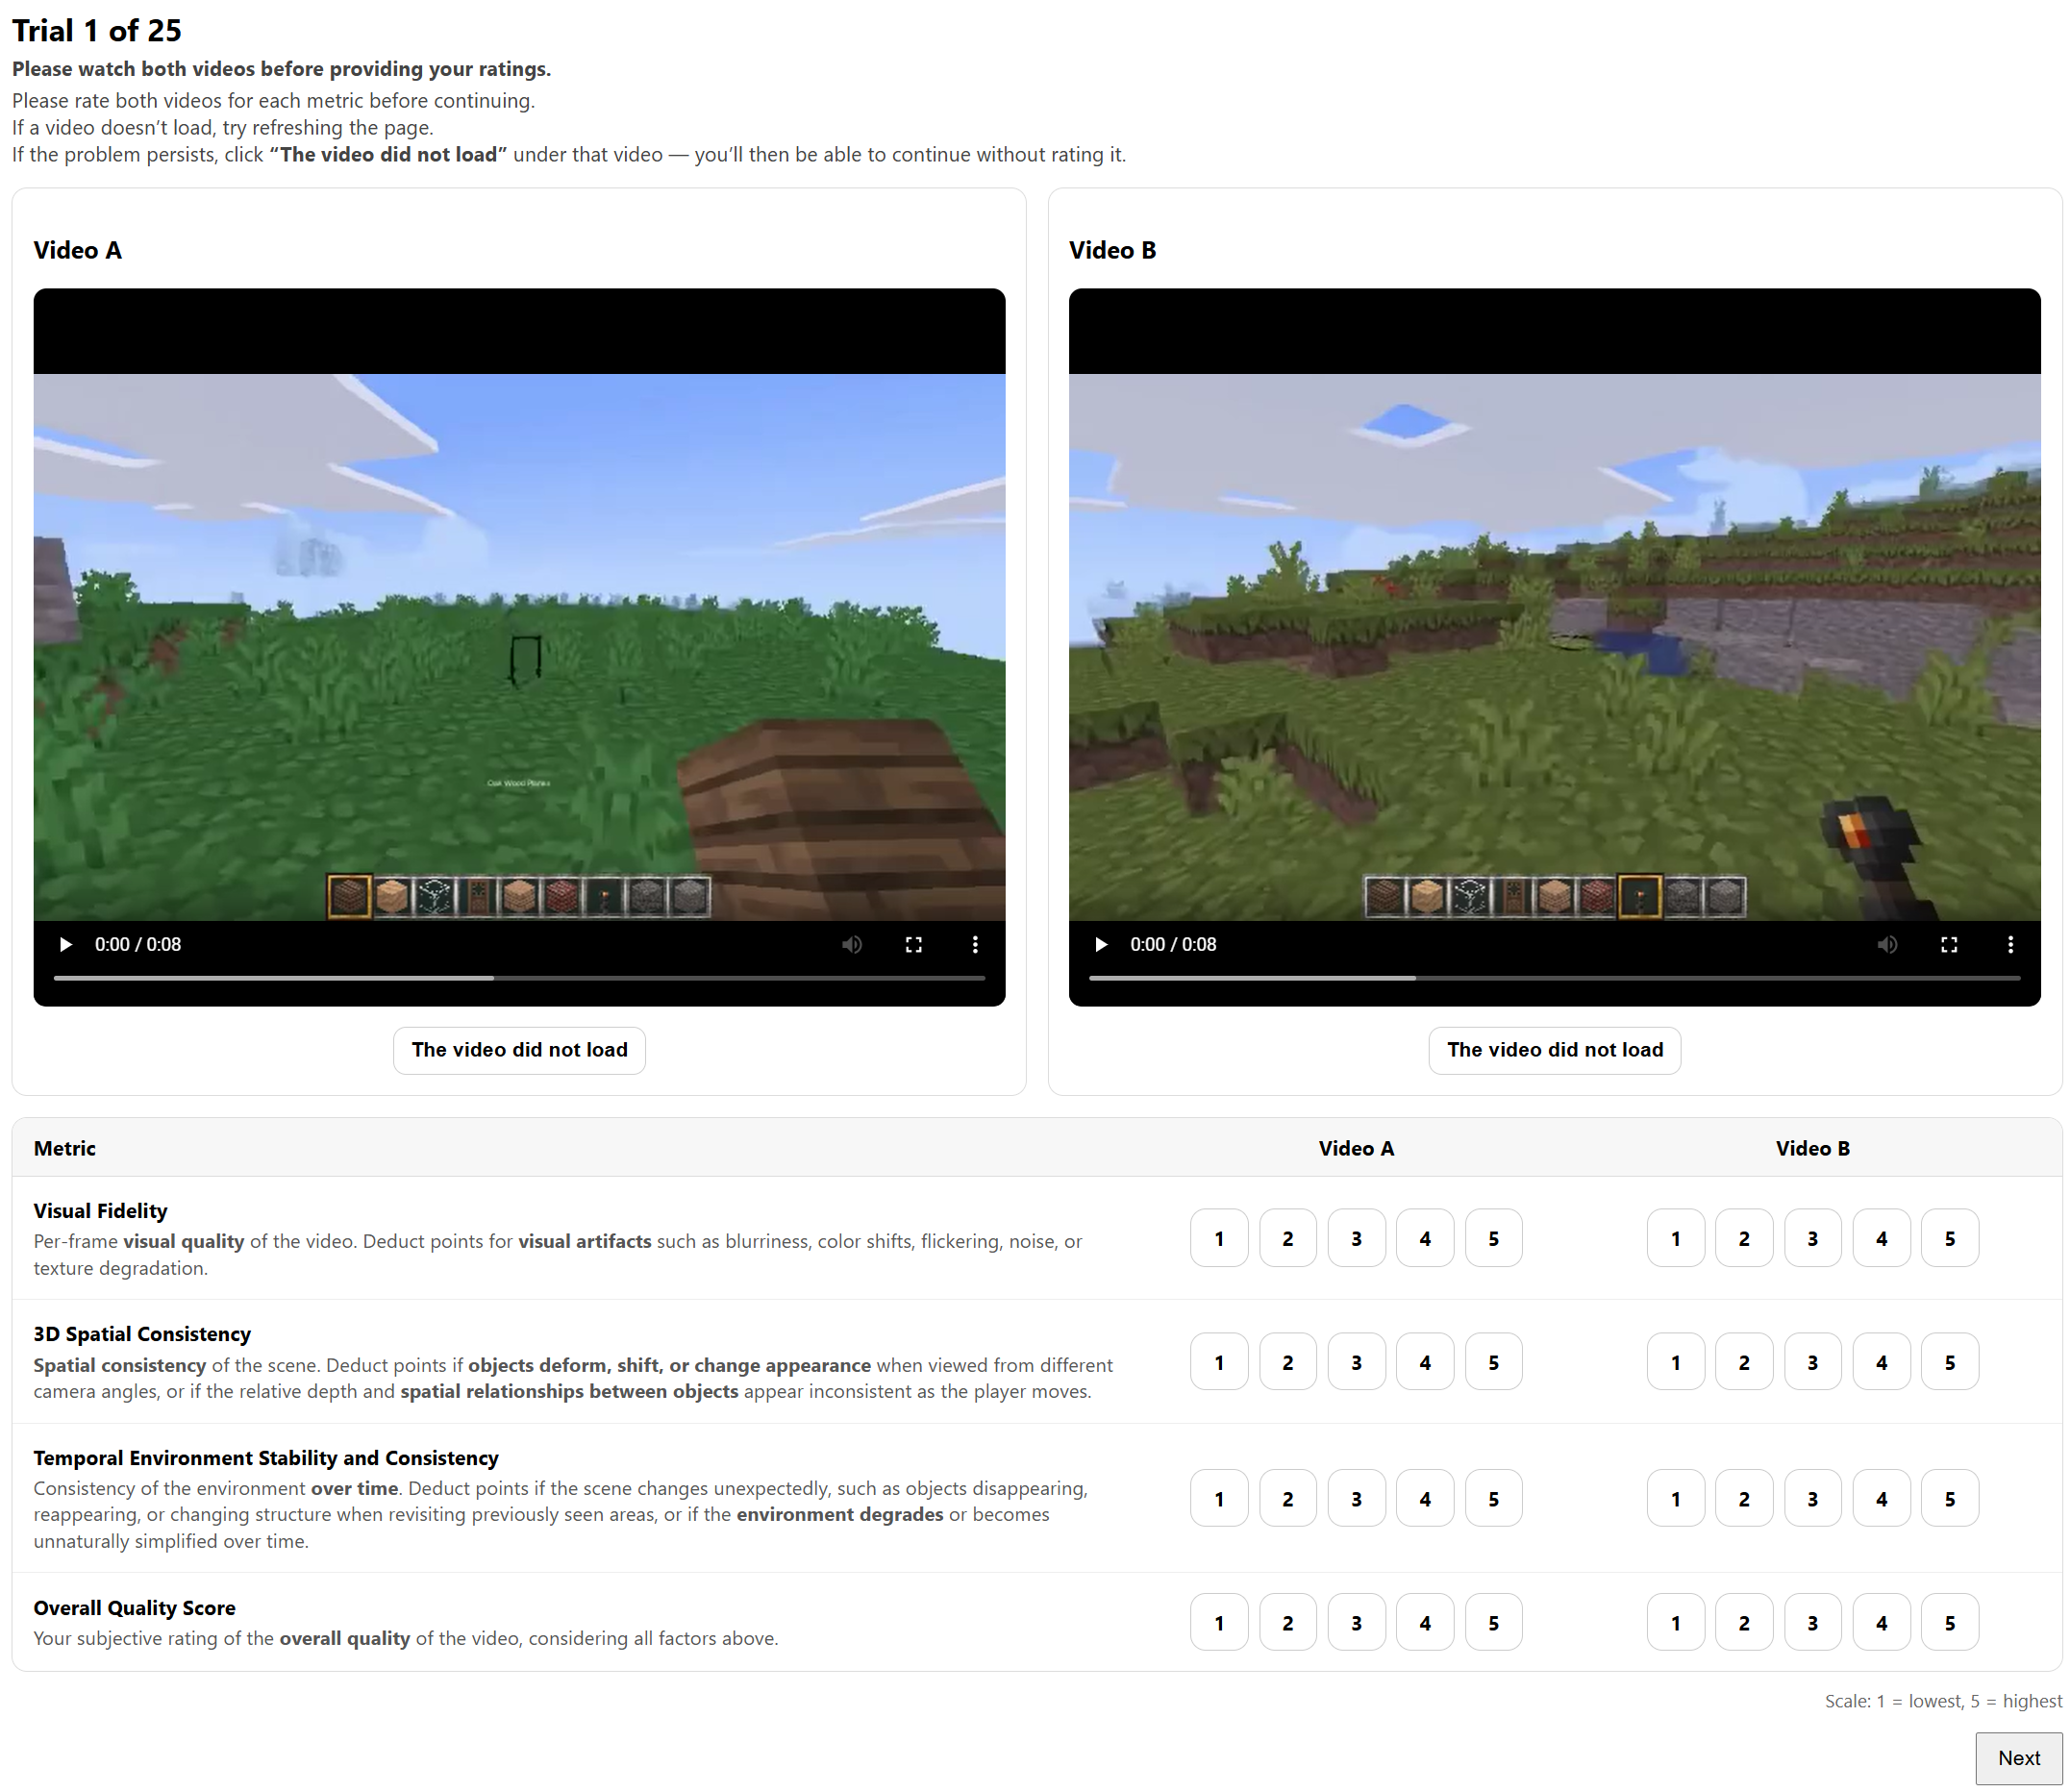
\includegraphics[width=1.0\linewidth]{figs/UI.png}
    \caption{\textbf{User Study Interface.} A screenshot of our web-based platform where participants evaluate video pairs based on temporal and spatial consistency.}
    \label{fig:ui_screenshot}
\DIFaddbeginFL \end{figure}

\section{\DIFadd{Extended User Study Results}}\label{app:ext_user_study}

\subsection{\DIFadd{Score Differences During Head-to-Head Comparisons}}
\DIFadd{Given that users rate two side-by-side videos during each trial, we can analyse how a PERSIST configuration fares in a direct head-to-head comparison against any other baseline, PERSIST configuration, or the ground truth data. We provide score comparison matrices below (one per metric) displaying the average score deltas during head-to-head comparisons.
}

\DIFadd{PERSIST configurations consistently outperform the baselines in every head-to-head comparison. During head-to-head comparisons between PERSIST-S and PERSIST-XL, PERSIST-S narrowly wins on 3D Spatial Consistency ($+0.21$), while PERSIST-XL achieves a slightly higher Overall Quality Score ($+0.14$). The differences in Visual Fidelity and Temporal Consistency are too narrow to call for either side. While PERSIST-XL achieves a better FVD, the results of the study indicate that humans do not observe a significant performance degradation when we decrease the number of spatial tokens allotted to $\gW_\theta$. In contrast, PERSIST-XL$+\vw_0$ wins most head-to-head comparisons against PERSIST-XL and PERSIST-S, which indicates that providing direct 3D conditioning generally improves performance. 
}

\DIFadd{Finally, users consistently prefer ground-truth videos across all metrics, highlighting that even our strongest configurations remain below the quality of real trajectories. This persistent gap underscores both the difficulty of long-horizon world modelling with procedurally generated environments, and the opportunity for further advances in persistent 3D generative representations.
}

\begin{figure*}[!htb]
  \begin{center}
    \centerline{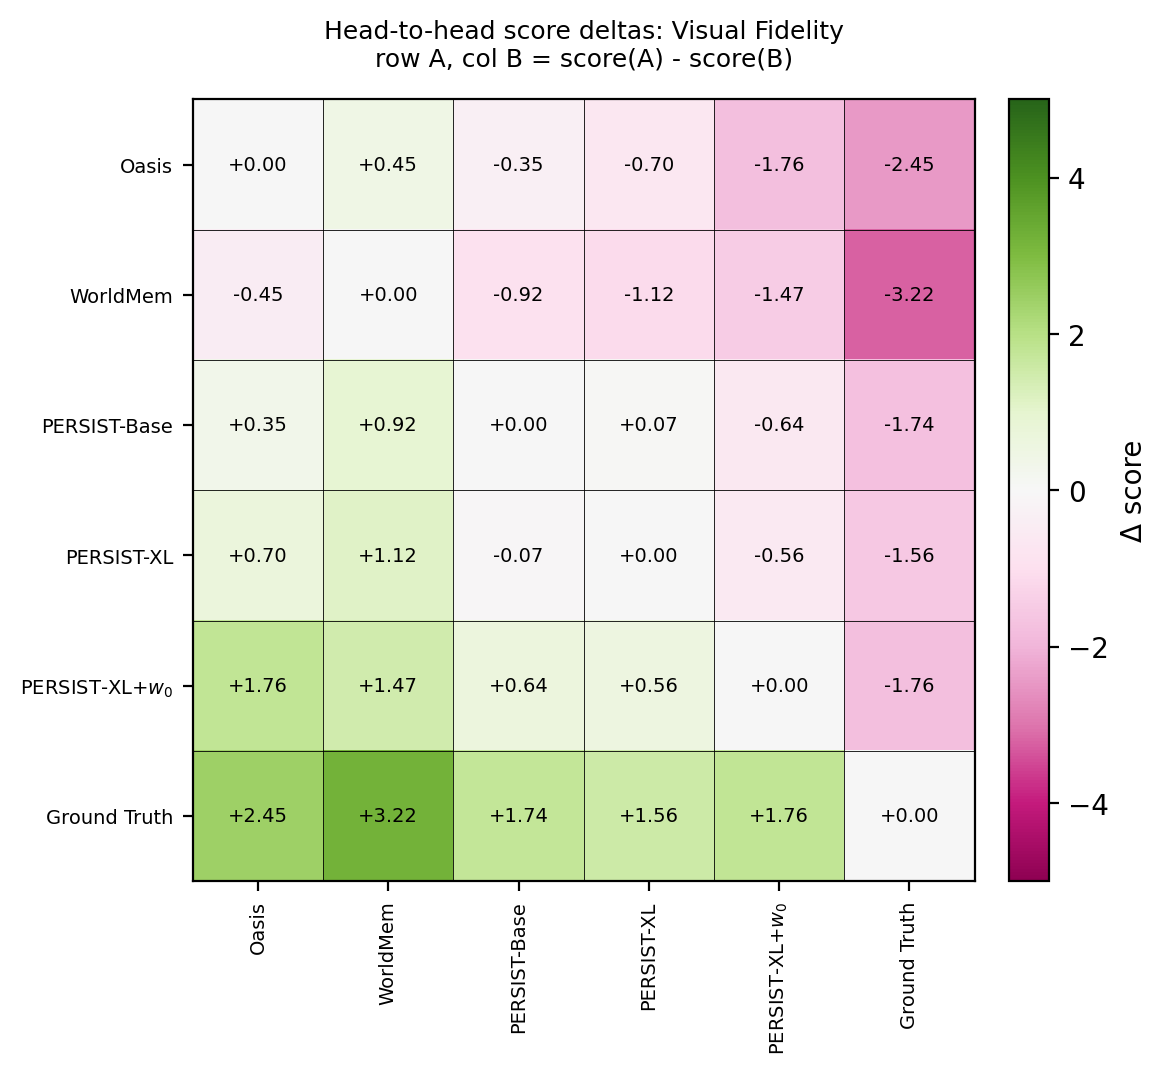
\includegraphics[width=0.85\linewidth]{figs/h2h_png/h2h_metric_a.png}}
    \caption{\DIFaddFL{Score differences during head-to-head comparisons, }\textbf{\DIFaddFL{visual fidelity}}\DIFaddFL{.}}
    \label{fig:hth_a}
  \end{center}
\end{figure*}

\begin{figure*}[!htb]
  \begin{center}
    \centerline{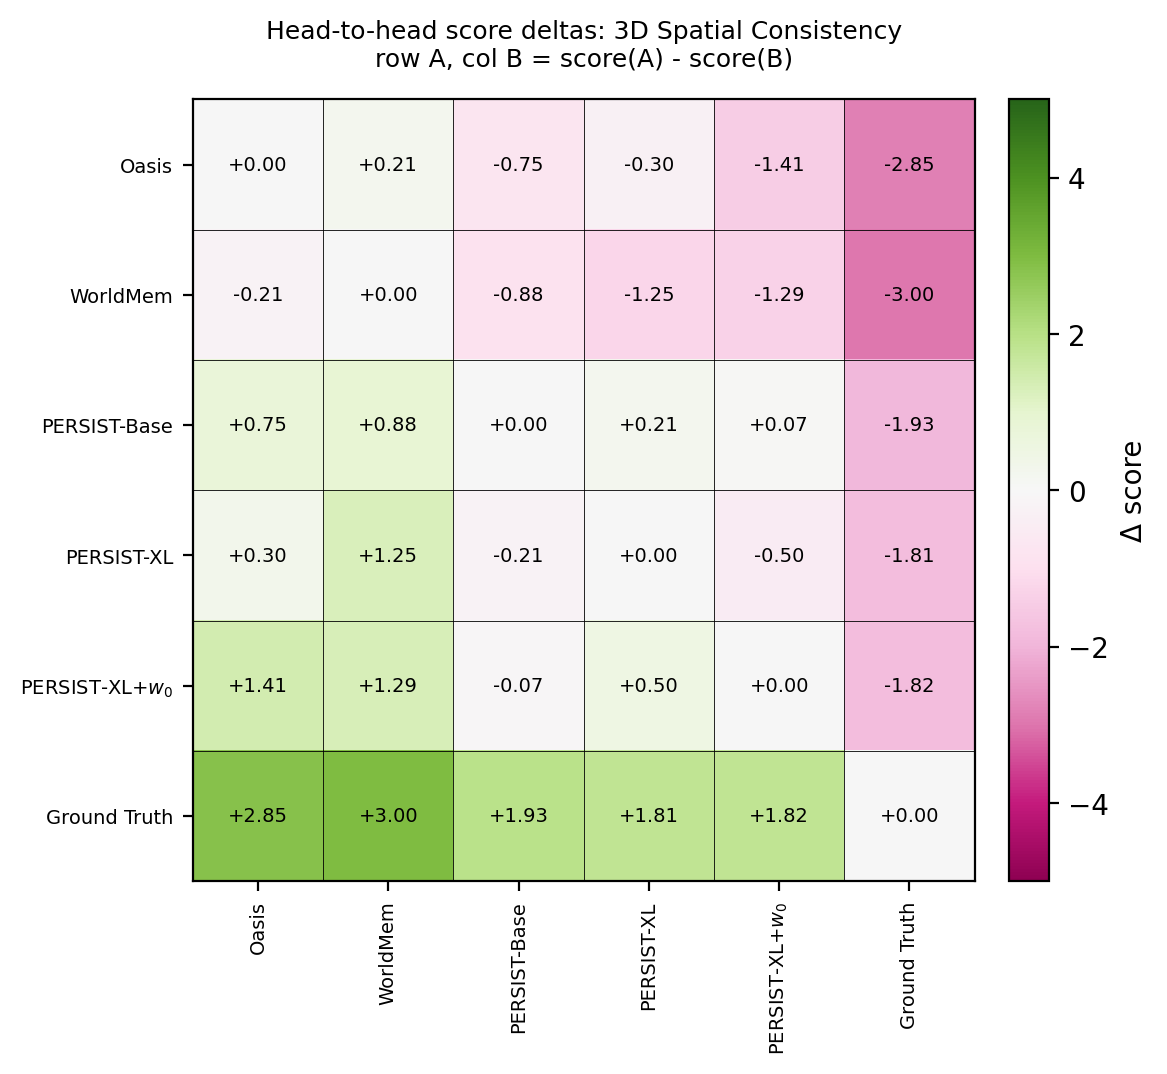
\includegraphics[width=0.85\linewidth]{figs/h2h_png/h2h_metric_b.png}}
    \caption{\DIFaddFL{Score differences during head-to-head comparisons, }\textbf{\DIFaddFL{3D spatial consistency}}\DIFaddFL{.}}
    \label{fig:hth_b}
  \end{center}
\end{figure*}

\begin{figure*}[!htb]
  \begin{center}
    \centerline{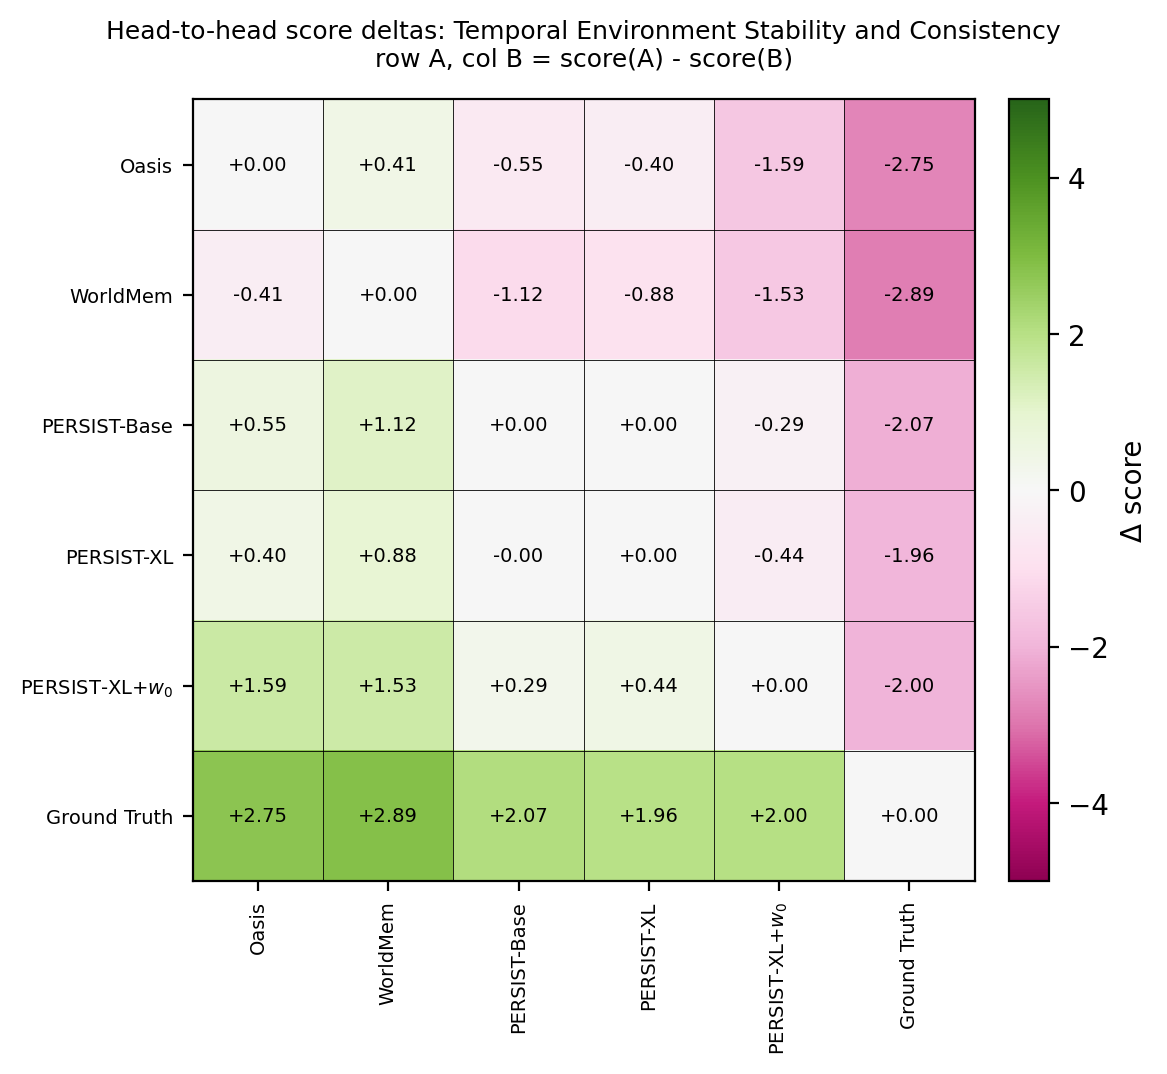
\includegraphics[width=0.85\linewidth]{figs/h2h_png/h2h_metric_c.png}}
    \caption{\DIFaddFL{Score differences during head-to-head comparisons, }\textbf{\DIFaddFL{temporal consistency}}\DIFaddFL{.}}
    \label{fig:hth_c}
  \end{center}
\end{figure*}

\begin{figure*}[!htb]
  \begin{center}
    \centerline{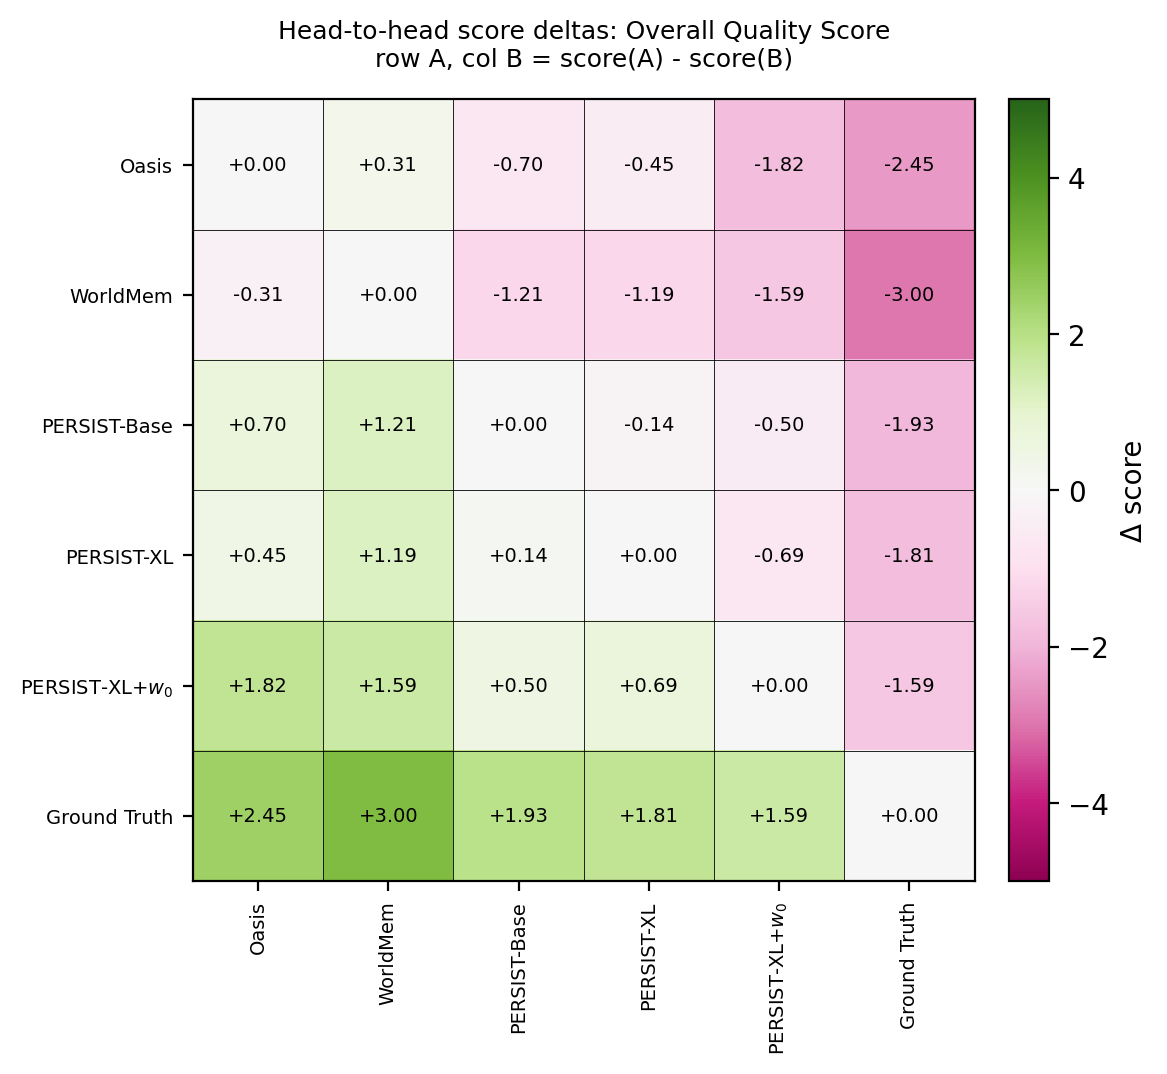
\includegraphics[width=0.85\linewidth]{figs/h2h_png/h2h_metric_d.png}}
    \caption{\DIFaddFL{Score differences during head-to-head comparisons, }\textbf{\DIFaddFL{overall quality score}}\DIFaddFL{.}}
    \label{fig:hth_d}
  \end{center}
\end{figure*}

\clearpage

\subsection{\DIFadd{Scores for Each Evaluation Set}}

\begin{table}[htb!]
\centering
\caption{\DIFaddFL{Per set user study scores: }\textbf{\DIFaddFL{circle around}}\DIFaddFL{.}}
\begin{tabular}{lcccc}
\toprule
\DIFaddFL{Method }& \DIFaddFL{Per Frame Visual Fidelity$\uparrow$ }& \DIFaddFL{3D Consistency$\uparrow$ }& \DIFaddFL{Temporal Consistency$\uparrow$ }& \DIFaddFL{Overall Score$\uparrow$ }\\
\midrule
\DIFaddFL{Oasis }& \DIFaddFL{2 $\pm$ 0.2 }& \DIFaddFL{1.6 $\pm$ 0.2 }& \DIFaddFL{1.5 $\pm$ 0.2 }& \DIFaddFL{1.6 $\pm$ 0.2 }\\
\DIFaddFL{WorldMem }& \DIFaddFL{1.7 $\pm$ 0.2 }& \DIFaddFL{1.5 $\pm$ 0.1 }& \DIFaddFL{1.3 $\pm$ 0.1 }& \DIFaddFL{1.4 $\pm$ 0.1 }\\
\DIFaddFL{PERSIST-S }& \DIFaddFL{2.8 $\pm$ 0.2 }& \DIFaddFL{2.6 $\pm$ 0.2 }& \DIFaddFL{2.3 $\pm$ 0.2 }& \DIFaddFL{2.5 $\pm$ 0.2 }\\
\DIFaddFL{PERSIST-XL }& \DIFaddFL{3.0 $\pm$ 0.2 }& \DIFaddFL{2.5 $\pm$ 0.1 }& \DIFaddFL{2.2 $\pm$ 0.1 }& \DIFaddFL{2.5 $\pm$ 0.1 }\\
\DIFaddFL{PERSIST-XL$+w_0$ }& \textbf{\DIFaddFL{3.4 $\pm$ 0.2}} & \textbf{\DIFaddFL{3.0 $\pm$ 0.2}} & \textbf{\DIFaddFL{2.7 $\pm$ 0.3}} & \textbf{\DIFaddFL{3.1 $\pm$ 0.2}} \\
\bottomrule
\end{tabular}
\label{tab:user_study_scores_circle_around}
\end{table}

\begin{table}[htb!]
\centering
\caption{\DIFaddFL{Per set user study scores: }\textbf{\DIFaddFL{free play}}\DIFaddFL{.}}
\label{tab:user_study_scores_free_play}
\begin{tabular}{lcccc}
\toprule
\DIFaddFL{Method }& \DIFaddFL{Per Frame Visual Fidelity$\uparrow$ }& \DIFaddFL{3D Consistency$\uparrow$ }& \DIFaddFL{Temporal Consistency$\uparrow$ }& \DIFaddFL{Overall Score$\uparrow$ }\\
\midrule
\DIFaddFL{Oasis }& \DIFaddFL{2.3 $\pm$ 0.2 }& \DIFaddFL{2.2 $\pm$ 0.2 }& \DIFaddFL{2.0 $\pm$ 0.2 }& \DIFaddFL{2.0 $\pm$ 0.2 }\\
\DIFaddFL{WorldMem }& \DIFaddFL{1.5 $\pm$ 0.2 }& \DIFaddFL{1.5 $\pm$ 0.2 }& \DIFaddFL{1.2 $\pm$ 0.1 }& \DIFaddFL{1.3 $\pm$ 0.1 }\\
\DIFaddFL{PERSIST-S }& \DIFaddFL{3.0 $\pm$ 0.2 }& \DIFaddFL{2.9 $\pm$ 0.2 }& \DIFaddFL{2.8 $\pm$ 0.2 }& \DIFaddFL{3.0 $\pm$ 0.2 }\\
\DIFaddFL{PERSIST-XL }& \DIFaddFL{2.9 $\pm$ 0.2 }& \DIFaddFL{2.8 $\pm$ 0.2 }& \DIFaddFL{2.8 $\pm$ 0.2 }& \DIFaddFL{2.8 $\pm$ 0.2 }\\
\DIFaddFL{PERSIST-XL$+w_0$ }& \textbf{\DIFaddFL{3.6 $\pm$ 0.2}} & \textbf{\DIFaddFL{3.1 $\pm$ 0.2}} & \textbf{\DIFaddFL{3.3 $\pm$ 0.2}} & \textbf{\DIFaddFL{3.4 $\pm$ 0.2}} \\
\bottomrule
\end{tabular}
\end{table}

\begin{table}[htb!]
\centering
\caption{\DIFaddFL{Per set user study scores: }\textbf{\DIFaddFL{backwards and look around}}\DIFaddFL{.}}\label{tab:user_study_scores_backward_and_look_around}
\begin{tabular}{lcccc}
\toprule
\DIFaddFL{Method }& \DIFaddFL{Per Frame Visual Fidelity$\uparrow$ }& \DIFaddFL{3D Consistency$\uparrow$ }& \DIFaddFL{Temporal Consistency$\uparrow$ }& \DIFaddFL{Overall Score$\uparrow$ }\\
\midrule
\DIFaddFL{Oasis }& \DIFaddFL{1.9 $\pm$ 0.2 }& \DIFaddFL{2.0 $\pm$ 0.2 }& \DIFaddFL{2.0 $\pm$ 0.2 }& \DIFaddFL{1.9 $\pm$ 0.2 }\\
\DIFaddFL{WorldMem }& \DIFaddFL{1.7 $\pm$ 0.2 }& \DIFaddFL{1.8 $\pm$ 0.2 }& \DIFaddFL{1.6 $\pm$ 0.2 }& \DIFaddFL{1.6 $\pm$ 0.1 }\\
\DIFaddFL{PERSIST-S }& \textbf{\DIFaddFL{3.0 $\pm$ 0.2}} & \textbf{\DIFaddFL{2.7 $\pm$ 0.2}} & \textbf{\DIFaddFL{2.7 $\pm$ 0.2}} & \DIFaddFL{2.6 $\pm$ 0.2 }\\
\DIFaddFL{PERSIST-XL }& \DIFaddFL{2.7 $\pm$ 0.2 }& \DIFaddFL{2.4 $\pm$ 0.2 }& \DIFaddFL{2.4 $\pm$ 0.2 }& \DIFaddFL{2.5 $\pm$ 0.1 }\\
\DIFaddFL{PERSIST-XL$+w_0$ }& \textbf{\DIFaddFL{3.0 $\pm$ 0.2}} & \DIFaddFL{2.6 $\pm$ 0.2 }& \DIFaddFL{2.6 $\pm$ 0.2 }& \textbf{\DIFaddFL{2.8 $\pm$ 0.2}} \\
\bottomrule
\end{tabular}
\end{table}

\begin{table}[htb!]
\caption{\DIFaddFL{Per set user study scores: }\textbf{\DIFaddFL{forward and look around}}\DIFaddFL{.}}
\label{tab:user_study_scores_forward_and_look_around}
\centering
\begin{tabular}{lcccc}
\toprule
\DIFaddFL{Method }& \DIFaddFL{Per Frame Visual Fidelity$\uparrow$ }& \DIFaddFL{3D Consistency$\uparrow$ }& \DIFaddFL{Temporal Consistency$\uparrow$ }& \DIFaddFL{Overall Score$\uparrow$ }\\
\midrule
\DIFaddFL{Oasis }& \DIFaddFL{2.4 $\pm$ 0.2 }& \DIFaddFL{2.0 $\pm$ 0.2 }& \DIFaddFL{1.8 $\pm$ 0.2 }& \DIFaddFL{1.9 $\pm$ 0.2 }\\
\DIFaddFL{WorldMem }& \DIFaddFL{2.1 $\pm$ 0.2 }& \DIFaddFL{2.2 $\pm$ 0.2 }& \DIFaddFL{1.9 $\pm$ 0.2 }& \DIFaddFL{1.9 $\pm$ 0.2 }\\
\DIFaddFL{PERSIST-S }& \DIFaddFL{2.2 $\pm$ 0.2 }& \DIFaddFL{2.3 $\pm$ 0.2 }& \DIFaddFL{2.1 $\pm$ 0.2 }& \DIFaddFL{2.3 $\pm$ 0.2 }\\
\DIFaddFL{PERSIST-XL }& \DIFaddFL{2.6 $\pm$ 0.2 }& \DIFaddFL{2.3 $\pm$ 0.2 }& \textbf{\DIFaddFL{2.3 $\pm$ 0.2}} & \textbf{\DIFaddFL{2.4 $\pm$ 0.1}} \\
\DIFaddFL{PERSIST-XL$+w_0$ }& \textbf{\DIFaddFL{2.7 $\pm$ 0.2}} & \textbf{\DIFaddFL{2.4 $\pm$ 0.2}} & \textbf{\DIFaddFL{2.3 $\pm$ 0.2}} & \textbf{\DIFaddFL{2.4 $\pm$ 0.2}} \\\bottomrule
\end{tabular}
\end{table}


%DIF >  \subsection{Cross domain evaluation}
%DIF >  \todo[inline]{This should be linked to in main text. Here we would briefly motivate why we believe the cross domain analysis with Minedojo \& Craftium is valid. Acknowledge FVD is not great to compare across different domains. However show: 1) similar upper bound for FVD. 2) Show Users assign same scores to Minedojo / Craftium ground truth data.}

\clearpage

\section{\DIFadd{Limitations and Future Work}}\label{app:limitations}

\textbf{\DIFadd{Training without ground truth 3D supervision.}} \DIFadd{Our results underscore the critical role of explicit 3D representations in maintaining environmental coherence over long horizons. Currently, however, PERSIST acquires this representation via supervised training, restricting its applicability to simulators or datasets providing 3D annotations~\mbox{%DIFAUXCMD
\citep[e.g.][]{zhou2018stereo,Matterport3D,yeshwanth2023scannet++}}\hskip0pt%DIFAUXCMD
. A key direction for future work is to relax this dependency by learning 3D representations directly from pixels, or by leveraging recent advances in 2D-to-3D foundation models~\mbox{%DIFAUXCMD
\citep{wang2025vggt,sam3dteam2025sam3d3dfyimages} }\hskip0pt%DIFAUXCMD
to generate synthetic 3D annotations as a pre-processing step.
}

\textbf{\DIFadd{Eliminating exposure bias.}} \DIFadd{While PERSIST yields substantial improvements in generation quality, temporal stability, and environmental coherence over baselines, human evaluators tend to prefer ground-truth videos in head-to-head comparisons, reporting a gradual degradation in visual quality and environment coherence over time. We attribute this degradation primarily to exposure bias: during training, individual pipeline components ($\gW_\theta$, $\gC_\theta$ and $\gP_\theta$) are trained using ground truth data; at inference, they condition on their own past predictions and on predictions from other components, causing a train-inference distribution mismatch that grows over time. We report examples of generation artifacts that occur over the course of a 2000 steps episode in \mbox{%DIFAUXCMD
\Cref{fig:limitations}}\hskip0pt%DIFAUXCMD
. Leveraging PERSIST's fully differentiable pipeline, future work could explore incorporating an end-to-end post-training stage on generated rollouts, thereby aligning the training and inference distributions. As demonstrated in recent work~\mbox{%DIFAUXCMD
\citep{huang2025self}}\hskip0pt%DIFAUXCMD
, this approach can be effective in making AR models robust to their own imperfect predictions.
}

\textbf{\DIFadd{Unconstrained spatial memory.}} \DIFadd{PERSIST presently tracks a finite region of 3D space centred on the agent, causing information from distant locations to be discarded as the agent moves through the environment. To retain spatial information over arbitrarily large environments, future work could consider a conditioning strategy for $\gW_\theta$ based on loading spatial chunks from a 3D memory bank. Whereas pixel memory banks suffer from viewpoint redundancy, a 3D store is inherently deduplicated and spatially organized, offering unique advantages for efficient storage and retrieval of spatial information.
}

\clearpage

\begin{figure*}[!htb]
  \begin{center}
    \centerline{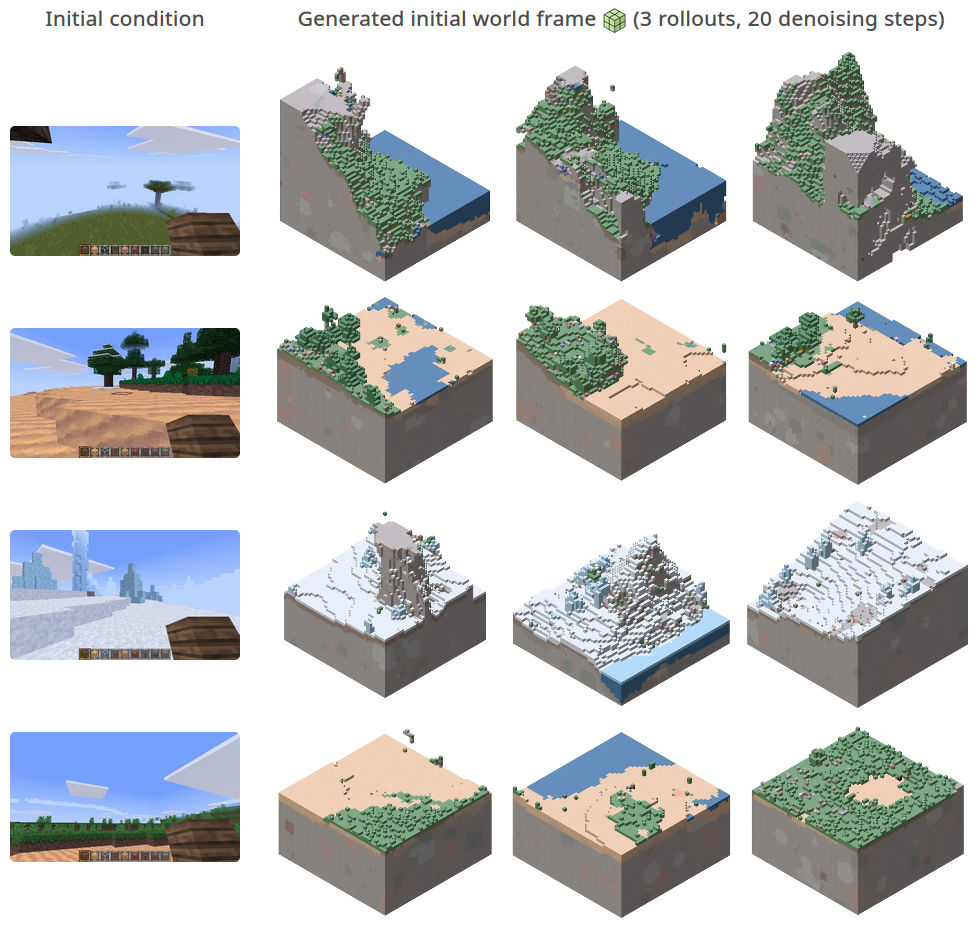
\includegraphics[width=0.85\linewidth]{figs/w0_generations.png}}
    \caption{\DIFaddFL{PERSIST generates diverse but coherent initial world frames from a single RGB conditioning observation. Each row corresponds to a specific input RGB frame, while each column depicts the initial world frame sampled from $\gW_\theta$ during a specific generation episode.}}
    \label{fig:w0_gen}
  \end{center}
\end{figure*}

\begin{figure}[!htb]
  \centering

  %DIF >  helper length: (optional) tighten vertical spacing between rows
  \begin{minipage}{0.7\linewidth}
        \setlength{\tabcolsep}{0pt}

  %DIF >  --- Row 1
  \noindent
  \begin{minipage}[c]{0.35\linewidth}
    \centering
    \begin{tcolorbox}[myimg,width=\linewidth]
    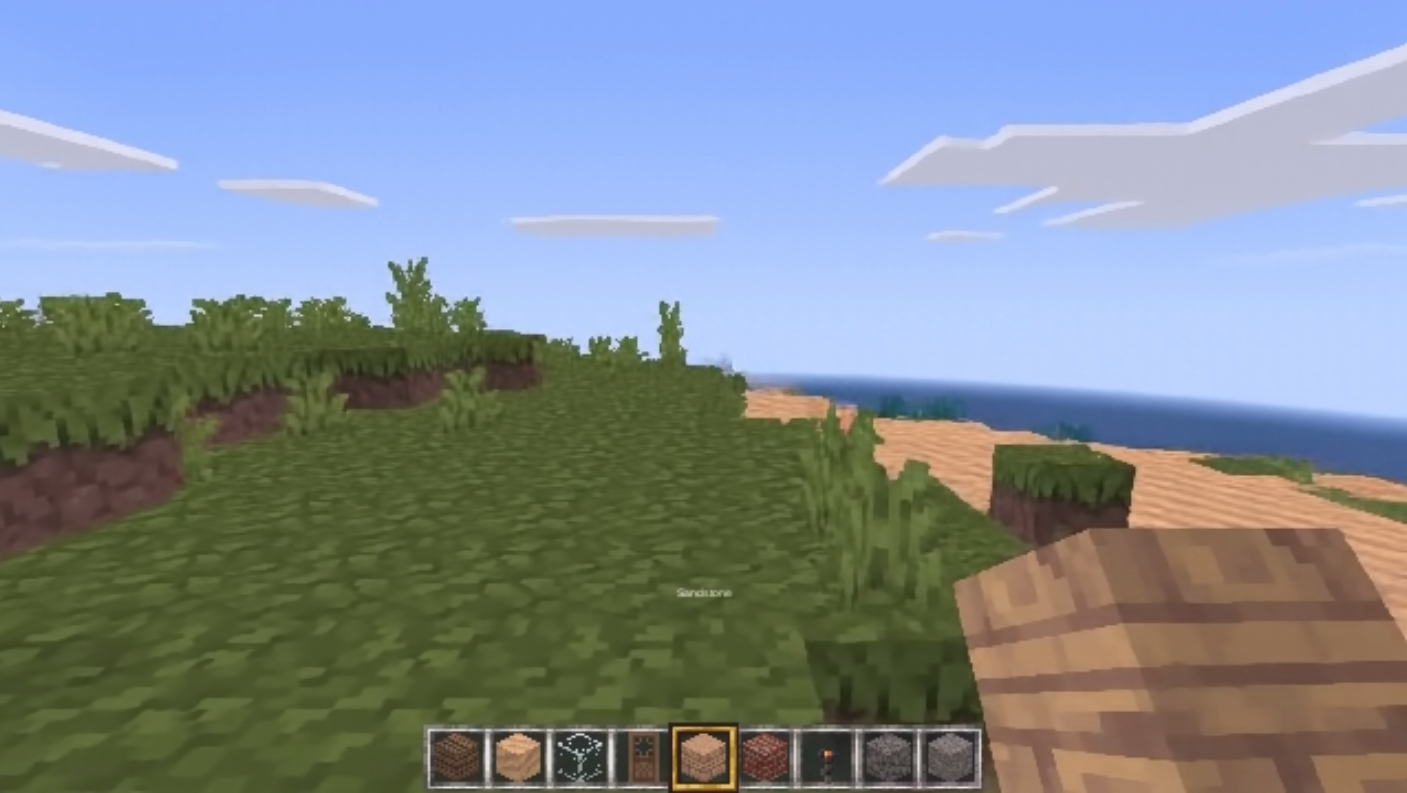
\includegraphics[width=\linewidth]{figs/limitations/s00.png}
    \end{tcolorbox}
  \end{minipage}\hfill
  \begin{minipage}[c]{0.55\linewidth}
    \textbf{\DIFaddFL{Step 0 (0 seconds)}}\DIFaddFL{. Start of the episode. Generation is stable.
  }\end{minipage}\par\vspace{0.6em}

  %DIF >  --- Row 2
  \noindent
  \begin{minipage}[c]{0.35\linewidth}
    \centering
    \begin{tcolorbox}[myimg,width=\linewidth]
    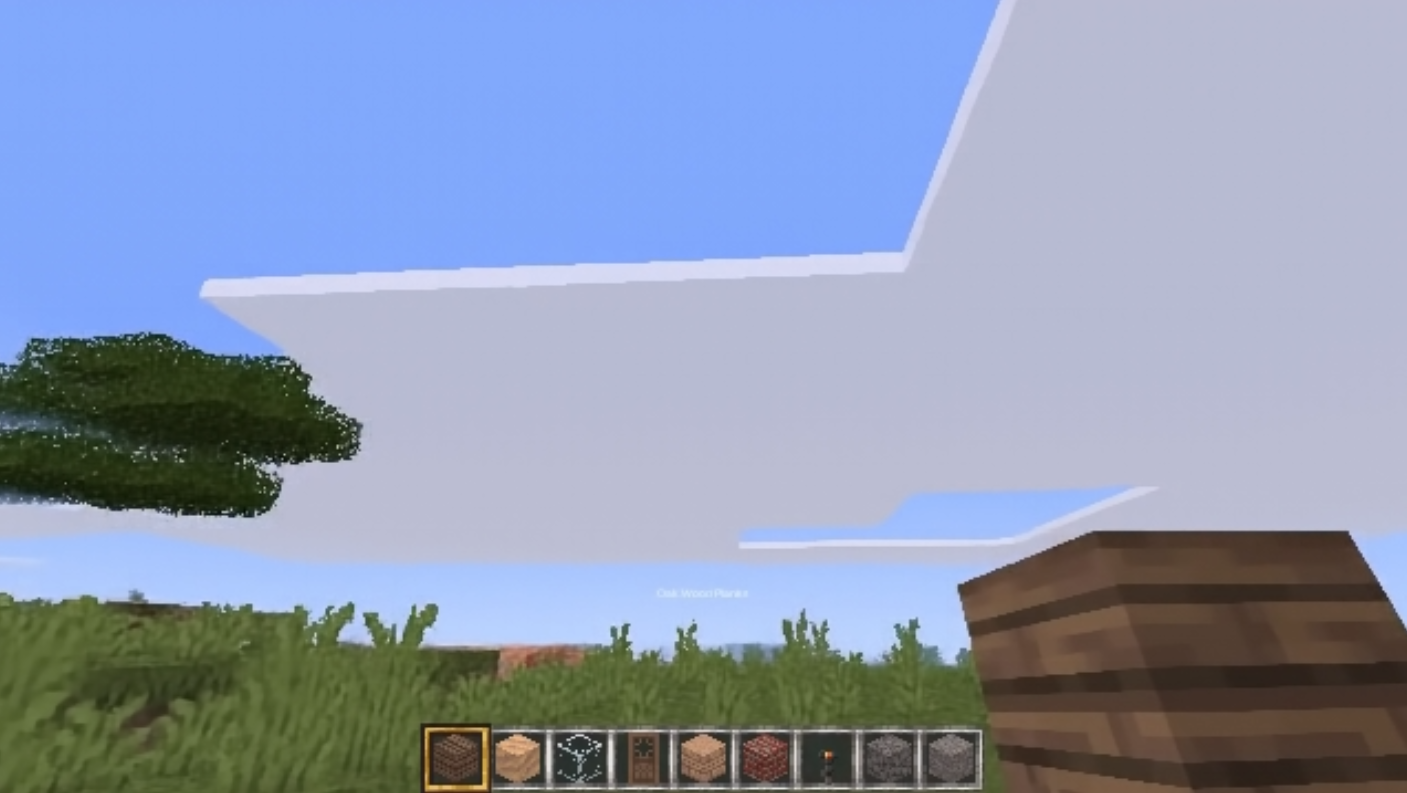
\includegraphics[width=\linewidth]{figs/limitations/s28.png}
    \end{tcolorbox}
  \end{minipage}\hfill
  \begin{minipage}[c]{0.55\linewidth}
    \textbf{\DIFaddFL{Step 672 (28 seconds)}}\DIFaddFL{. A tree trunk disappears from the 3D representation. As a result only the tree foliage is rendered to the left of the agent.
  }\end{minipage}\par\vspace{0.6em}

  %DIF >  --- Row 3
  \noindent
  \begin{minipage}[c]{0.35\linewidth}
    \centering
    \begin{tcolorbox}[myimg,width=\linewidth]
    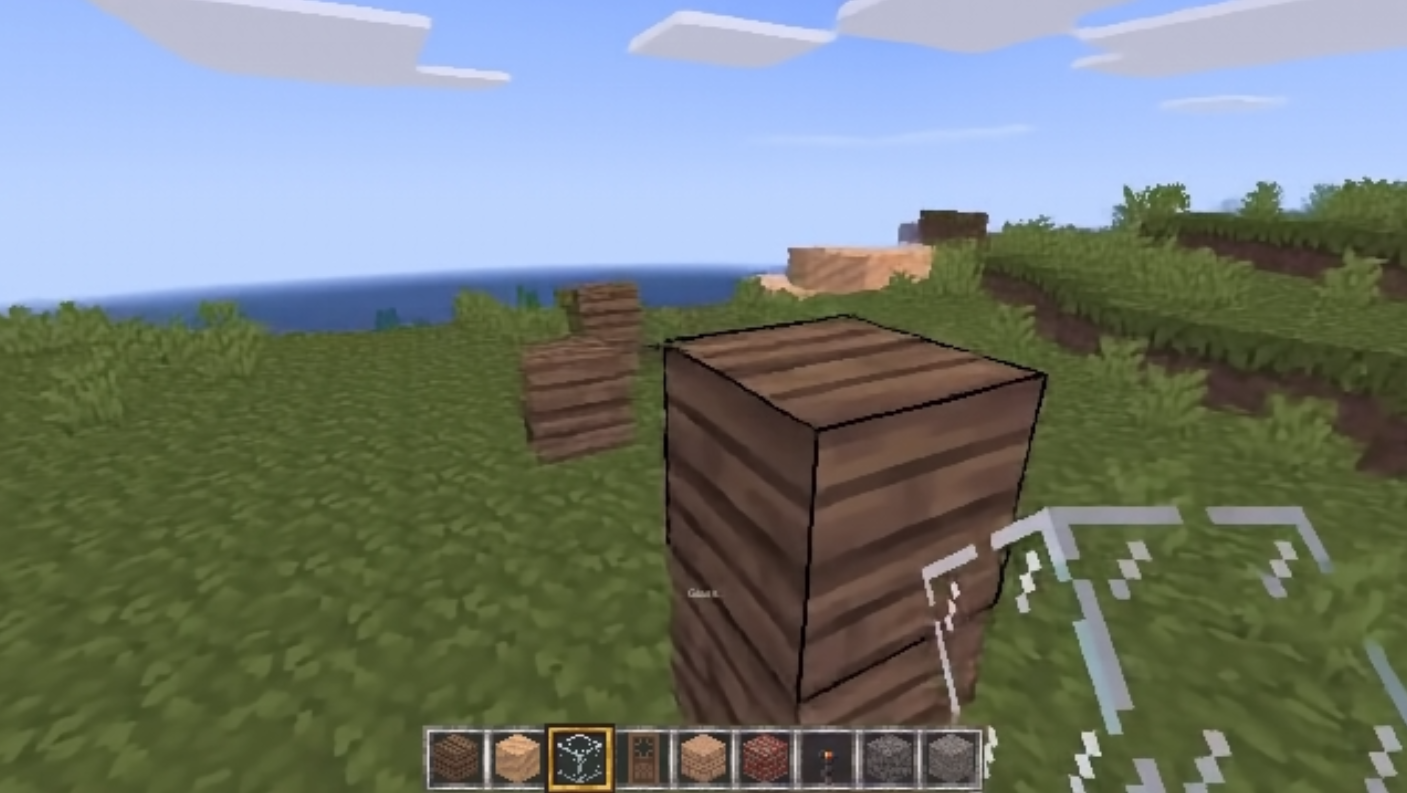
\includegraphics[width=\linewidth]{figs/limitations/s37.png}
    \end{tcolorbox}
  \end{minipage}\hfill
  \begin{minipage}[c]{0.55\linewidth}
    \textbf{\DIFaddFL{Step 888 (37 seconds)}}\DIFaddFL{. Several wood blocs are wrongly predicted by $\gW_\vtheta$ and appear in the 3D representation. They get rendered in the agent's view.
  }\end{minipage}\par\vspace{0.6em}

  %DIF >  --- Row 4
  \noindent
  \begin{minipage}[c]{0.35\linewidth}
    \centering
    \begin{tcolorbox}[myimg,width=\linewidth]
    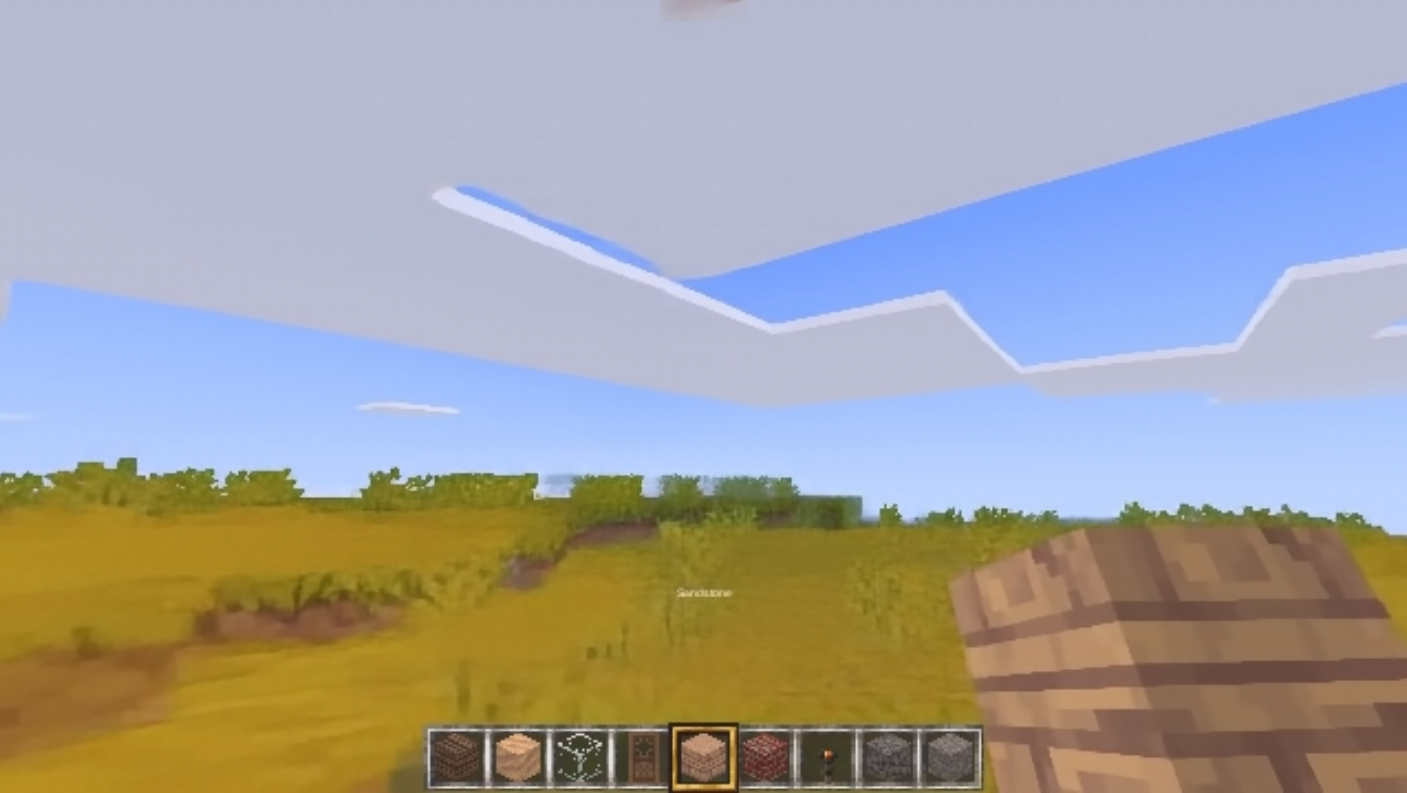
\includegraphics[width=\linewidth]{figs/limitations/s54.png}
    \end{tcolorbox}
  \end{minipage}\hfill
  \begin{minipage}[c]{0.55\linewidth}
    \textbf{\DIFaddFL{Step 1296 (54 seconds)}}\DIFaddFL{. The texture of the ground is drifting to a yellowish colour. The 3D representation remains stable.
  }\end{minipage}\par\vspace{0.6em}

  %DIF >  --- Row 5
  \noindent
  \begin{minipage}[c]{0.35\linewidth}
    \centering
    \begin{tcolorbox}[myimg,width=\linewidth]
    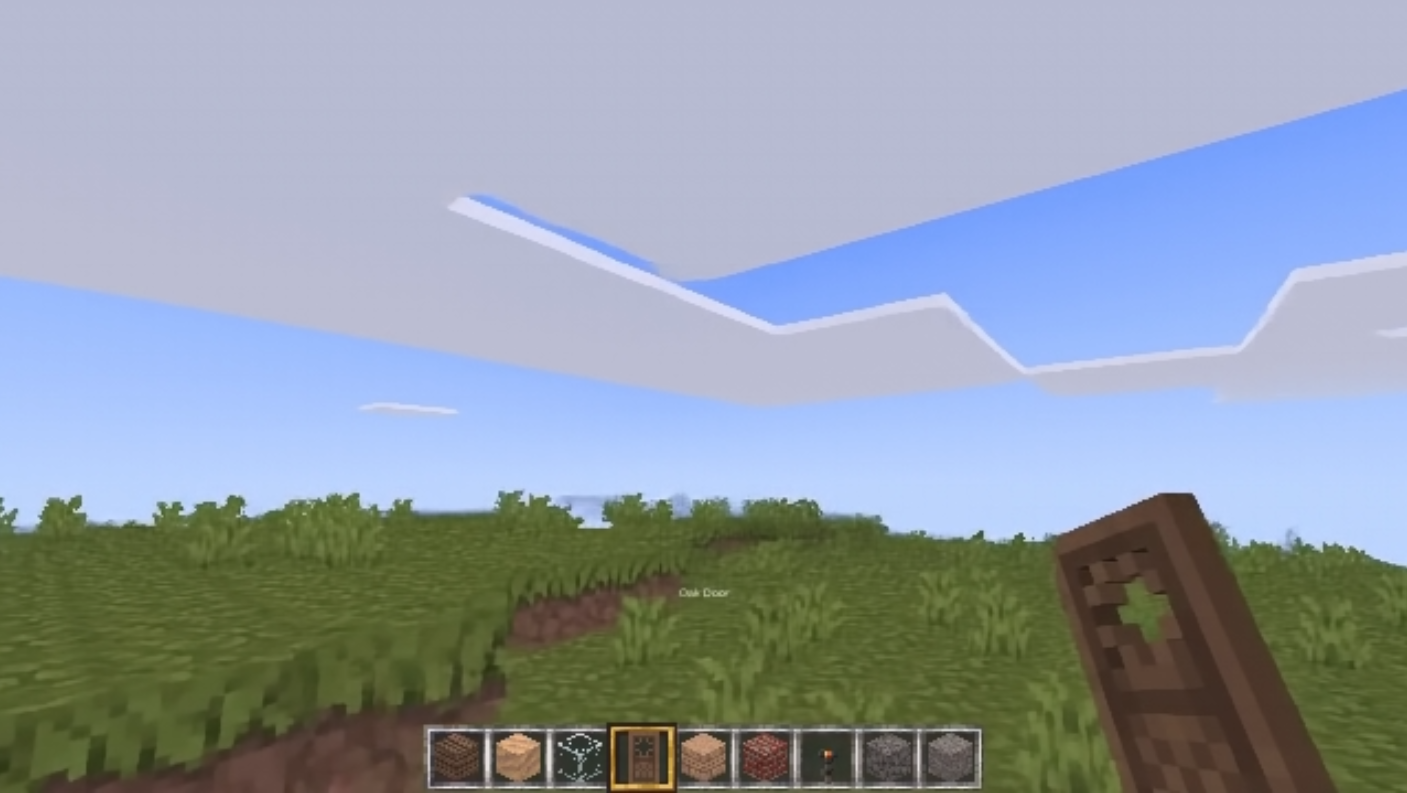
\includegraphics[width=\linewidth]{figs/limitations/s55.png}
    \end{tcolorbox}
  \end{minipage}\hfill
  \begin{minipage}[c]{0.55\linewidth}
    \textbf{\DIFaddFL{Step 1320 (55 seconds)}}\DIFaddFL{. $\gP_\vtheta$ recovers the correct texture thanks to the grounding provided by $\vw_{2D}$.
  }\end{minipage}\par\vspace{0.6em}

  %DIF >  --- Row 6
  \noindent
  \begin{minipage}[c]{0.35\linewidth}
    \centering
    \begin{tcolorbox}[myimg,width=\linewidth]
    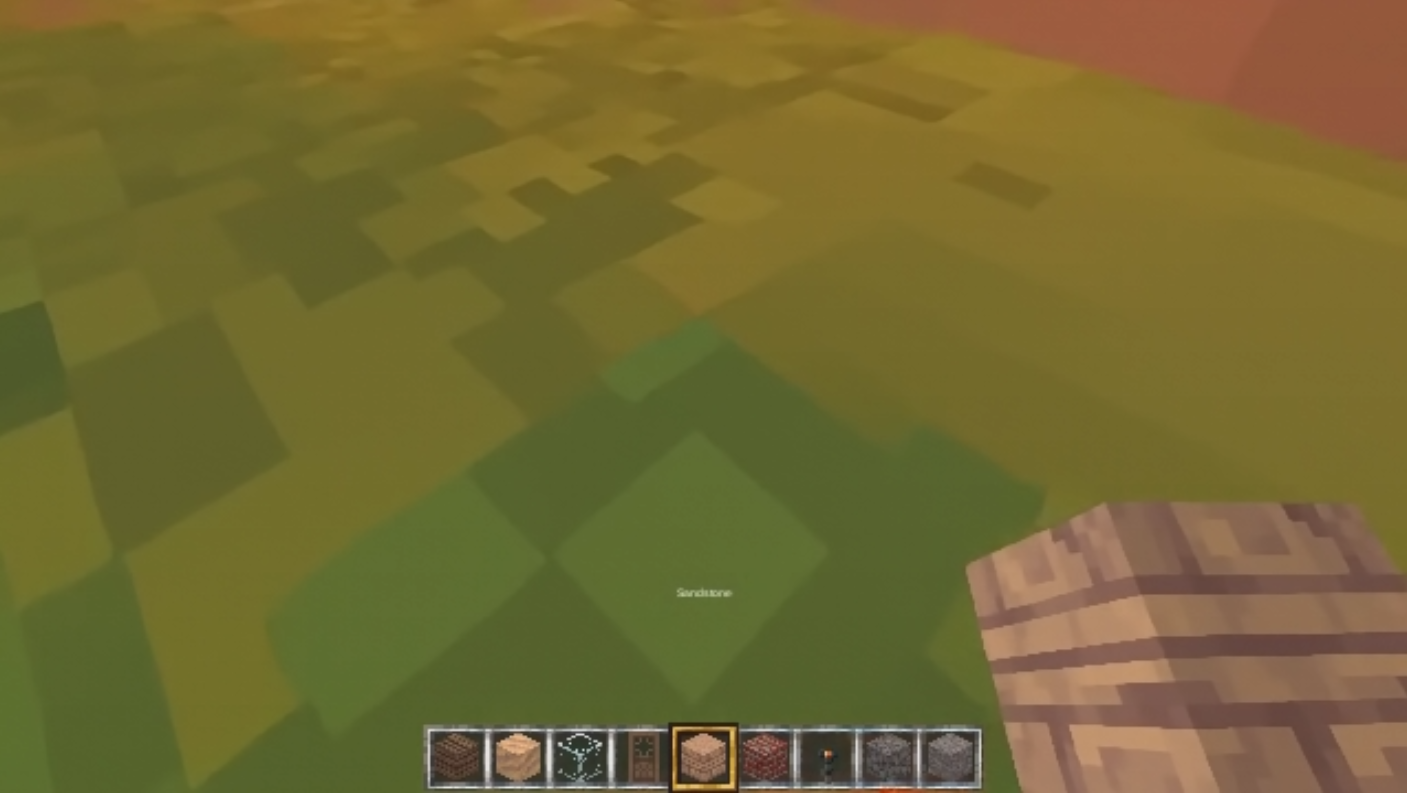
\includegraphics[width=\linewidth]{figs/limitations/s69.png}
    \end{tcolorbox}
  \end{minipage}\hfill
  \begin{minipage}[c]{0.55\linewidth}
    \textbf{\DIFaddFL{Step 1656 (69 seconds)}}\DIFaddFL{. A collision gets mispredicted and the agent clips through a bloc. The ground texture begins to drift.
  }\end{minipage}\par\vspace{0.6em}

  %DIF >  --- Row 7
  \noindent
  \begin{minipage}[c]{0.35\linewidth}
    \centering
    \begin{tcolorbox}[myimg,width=\linewidth]
    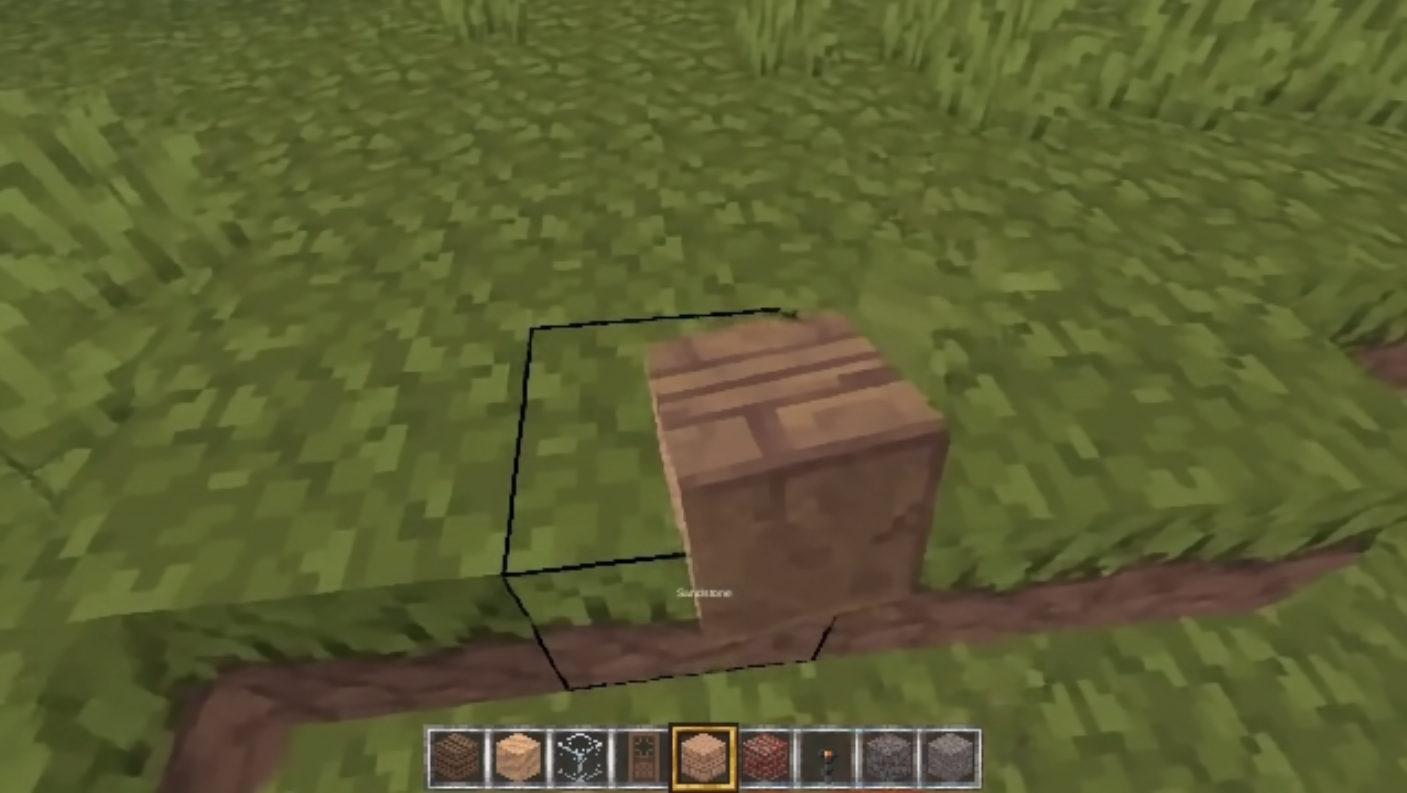
\includegraphics[width=\linewidth]{figs/limitations/s70.png}
    \end{tcolorbox}
  \end{minipage}\hfill
  \begin{minipage}[c]{0.55\linewidth}
    \textbf{\DIFaddFL{Step 1680 (70 seconds)}}\DIFaddFL{. The model recovers from terrain clip
    ping and texture drift after the agent executes a jump action.
  }\end{minipage}\par\vspace{0.6em}

  %DIF >  --- Row 8
  \noindent
  \begin{minipage}[c]{0.35\linewidth}
    \centering
    \begin{tcolorbox}[myimg,width=\linewidth]
    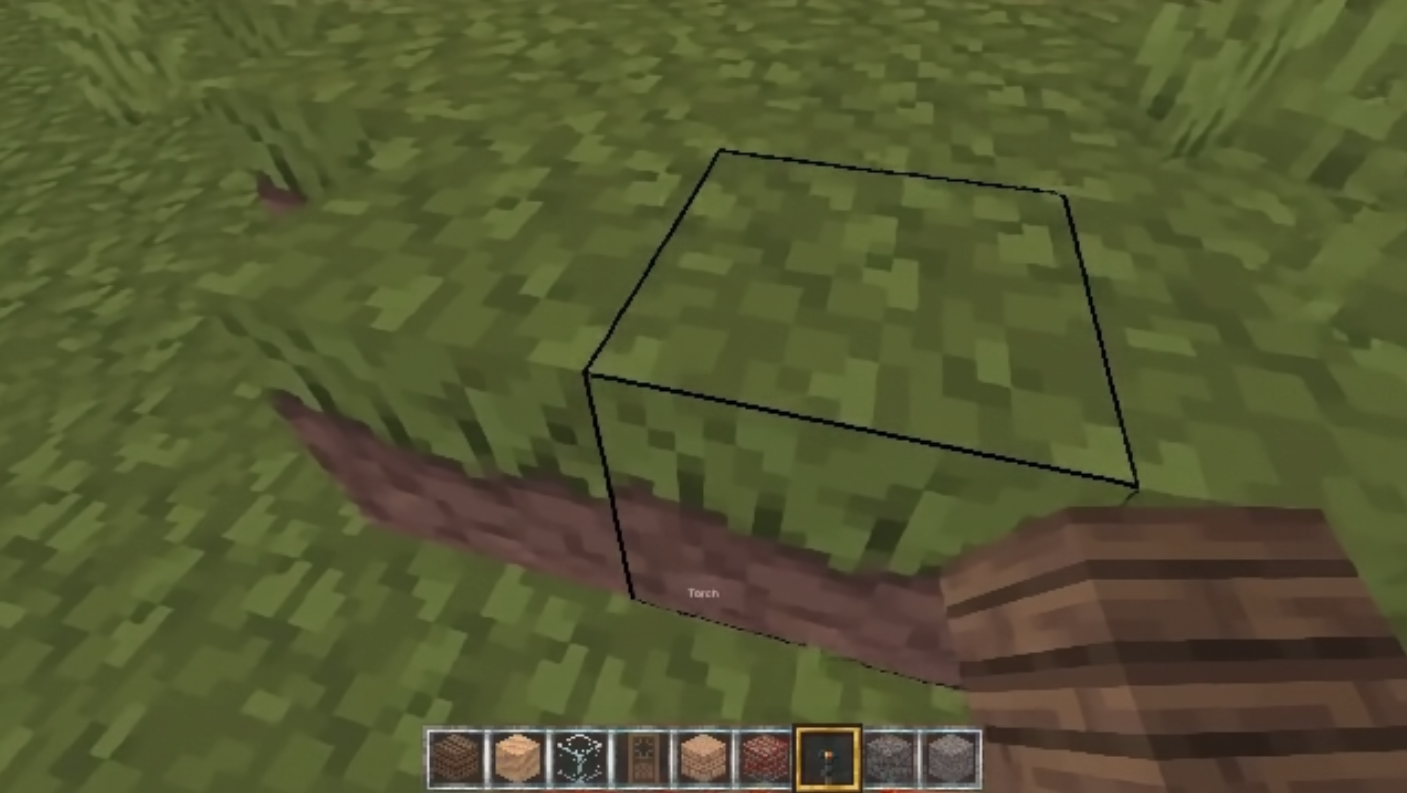
\includegraphics[width=\linewidth]{figs/limitations/s83.png}
    \end{tcolorbox}
  \end{minipage}\hfill
  \begin{minipage}[c]{0.55\linewidth}
    \textbf{\DIFaddFL{Step 2000 (83 seconds)}}\DIFaddFL{. The episode concludes on a stable frame. The environment remains globally coherent after 2000 steps, but artifacts occur more frequently due to exposure bias.
  }\end{minipage}
  \end{minipage}

\vspace{0.25cm}
  \caption{\DIFaddFL{Generation artifacts and subsequent recoveries over a 2000 step (83 seconds) episode generated with PERSIST. The 3D representation drifts locally, causing individual blocs to appear and disappear from the agent's view. However we find that the 3D representation remains globally coherent and has a net stabilising effect on generation, allowing $\gP_\theta$ to recover from visual artifacts. This lets PERSIST generate rollouts lasting thousands of steps, even if glitches become more frequent over time due to autoregressive drift.}}
  \label{fig:limitations}
\DIFaddendFL \end{figure}

%%%%%%%%%%%%%%%%%%%%%%%%%%%%%%%%%%%%%%%%%%%%%%%%%%%%%%%%%%%%%%%%%%%%%%%%%%%%%%%
%%%%%%%%%%%%%%%%%%%%%%%%%%%%%%%%%%%%%%%%%%%%%%%%%%%%%%%%%%%%%%%%%%%%%%%%%%%%%%%

\end{document}

% This document was modified from the file originally made available by
% Pat Langley and Andrea Danyluk for ICML-2K. This version was created
% by Iain Murray in 2018, and modified by Alexandre Bouchard in
% 2019 and 2021 and by Csaba Szepesvari, Gang Niu and Sivan Sabato in 2022.
% Modified again in 2023 and 2024 by Sivan Sabato and Jonathan Scarlett.
% Previous contributors include Dan Roy, Lise Getoor and Tobias
% Scheffer, which was slightly modified from the 2010 version by
% Thorsten Joachims & Johannes Fuernkranz, slightly modified from the
% 2009 version by Kiri Wagstaff and Sam Roweis's 2008 version, which is
% slightly modified from Prasad Tadepalli's 2007 version which is a
% lightly changed version of the previous year's version by Andrew
% Moore, which was in turn edited from those of Kristian Kersting and
% Codrina Lauth. Alex Smola contributed to the algorithmic style files.
